% Options for packages loaded elsewhere
\PassOptionsToPackage{unicode}{hyperref}
\PassOptionsToPackage{hyphens}{url}
%
\documentclass[
  twoside]{article}
\usepackage{amsmath,amssymb}
\usepackage{iftex}
\ifPDFTeX
  \usepackage[T1]{fontenc}
  \usepackage[utf8]{inputenc}
  \usepackage{textcomp} % provide euro and other symbols
\else % if luatex or xetex
  \usepackage{unicode-math} % this also loads fontspec
  \defaultfontfeatures{Scale=MatchLowercase}
  \defaultfontfeatures[\rmfamily]{Ligatures=TeX,Scale=1}
\fi
\usepackage{lmodern}
\ifPDFTeX\else
  % xetex/luatex font selection
\fi
% Use upquote if available, for straight quotes in verbatim environments
\IfFileExists{upquote.sty}{\usepackage{upquote}}{}
\IfFileExists{microtype.sty}{% use microtype if available
  \usepackage[]{microtype}
  \UseMicrotypeSet[protrusion]{basicmath} % disable protrusion for tt fonts
}{}
\makeatletter
\@ifundefined{KOMAClassName}{% if non-KOMA class
  \IfFileExists{parskip.sty}{%
    \usepackage{parskip}
  }{% else
    \setlength{\parindent}{0pt}
    \setlength{\parskip}{6pt plus 2pt minus 1pt}}
}{% if KOMA class
  \KOMAoptions{parskip=half}}
\makeatother
\usepackage{xcolor}
\usepackage[margin=1in]{geometry}
\usepackage{color}
\usepackage{fancyvrb}
\newcommand{\VerbBar}{|}
\newcommand{\VERB}{\Verb[commandchars=\\\{\}]}
\DefineVerbatimEnvironment{Highlighting}{Verbatim}{commandchars=\\\{\}}
% Add ',fontsize=\small' for more characters per line
\usepackage{framed}
\definecolor{shadecolor}{RGB}{248,248,248}
\newenvironment{Shaded}{\begin{snugshade}}{\end{snugshade}}
\newcommand{\AlertTok}[1]{\textcolor[rgb]{0.94,0.16,0.16}{#1}}
\newcommand{\AnnotationTok}[1]{\textcolor[rgb]{0.56,0.35,0.01}{\textbf{\textit{#1}}}}
\newcommand{\AttributeTok}[1]{\textcolor[rgb]{0.13,0.29,0.53}{#1}}
\newcommand{\BaseNTok}[1]{\textcolor[rgb]{0.00,0.00,0.81}{#1}}
\newcommand{\BuiltInTok}[1]{#1}
\newcommand{\CharTok}[1]{\textcolor[rgb]{0.31,0.60,0.02}{#1}}
\newcommand{\CommentTok}[1]{\textcolor[rgb]{0.56,0.35,0.01}{\textit{#1}}}
\newcommand{\CommentVarTok}[1]{\textcolor[rgb]{0.56,0.35,0.01}{\textbf{\textit{#1}}}}
\newcommand{\ConstantTok}[1]{\textcolor[rgb]{0.56,0.35,0.01}{#1}}
\newcommand{\ControlFlowTok}[1]{\textcolor[rgb]{0.13,0.29,0.53}{\textbf{#1}}}
\newcommand{\DataTypeTok}[1]{\textcolor[rgb]{0.13,0.29,0.53}{#1}}
\newcommand{\DecValTok}[1]{\textcolor[rgb]{0.00,0.00,0.81}{#1}}
\newcommand{\DocumentationTok}[1]{\textcolor[rgb]{0.56,0.35,0.01}{\textbf{\textit{#1}}}}
\newcommand{\ErrorTok}[1]{\textcolor[rgb]{0.64,0.00,0.00}{\textbf{#1}}}
\newcommand{\ExtensionTok}[1]{#1}
\newcommand{\FloatTok}[1]{\textcolor[rgb]{0.00,0.00,0.81}{#1}}
\newcommand{\FunctionTok}[1]{\textcolor[rgb]{0.13,0.29,0.53}{\textbf{#1}}}
\newcommand{\ImportTok}[1]{#1}
\newcommand{\InformationTok}[1]{\textcolor[rgb]{0.56,0.35,0.01}{\textbf{\textit{#1}}}}
\newcommand{\KeywordTok}[1]{\textcolor[rgb]{0.13,0.29,0.53}{\textbf{#1}}}
\newcommand{\NormalTok}[1]{#1}
\newcommand{\OperatorTok}[1]{\textcolor[rgb]{0.81,0.36,0.00}{\textbf{#1}}}
\newcommand{\OtherTok}[1]{\textcolor[rgb]{0.56,0.35,0.01}{#1}}
\newcommand{\PreprocessorTok}[1]{\textcolor[rgb]{0.56,0.35,0.01}{\textit{#1}}}
\newcommand{\RegionMarkerTok}[1]{#1}
\newcommand{\SpecialCharTok}[1]{\textcolor[rgb]{0.81,0.36,0.00}{\textbf{#1}}}
\newcommand{\SpecialStringTok}[1]{\textcolor[rgb]{0.31,0.60,0.02}{#1}}
\newcommand{\StringTok}[1]{\textcolor[rgb]{0.31,0.60,0.02}{#1}}
\newcommand{\VariableTok}[1]{\textcolor[rgb]{0.00,0.00,0.00}{#1}}
\newcommand{\VerbatimStringTok}[1]{\textcolor[rgb]{0.31,0.60,0.02}{#1}}
\newcommand{\WarningTok}[1]{\textcolor[rgb]{0.56,0.35,0.01}{\textbf{\textit{#1}}}}
\usepackage{graphicx}
\makeatletter
\def\maxwidth{\ifdim\Gin@nat@width>\linewidth\linewidth\else\Gin@nat@width\fi}
\def\maxheight{\ifdim\Gin@nat@height>\textheight\textheight\else\Gin@nat@height\fi}
\makeatother
% Scale images if necessary, so that they will not overflow the page
% margins by default, and it is still possible to overwrite the defaults
% using explicit options in \includegraphics[width, height, ...]{}
\setkeys{Gin}{width=\maxwidth,height=\maxheight,keepaspectratio}
% Set default figure placement to htbp
\makeatletter
\def\fps@figure{htbp}
\makeatother
\setlength{\emergencystretch}{3em} % prevent overfull lines
\providecommand{\tightlist}{%
  \setlength{\itemsep}{0pt}\setlength{\parskip}{0pt}}
\setcounter{secnumdepth}{5}
\ifLuaTeX
  \usepackage{selnolig}  % disable illegal ligatures
\fi
\IfFileExists{bookmark.sty}{\usepackage{bookmark}}{\usepackage{hyperref}}
\IfFileExists{xurl.sty}{\usepackage{xurl}}{} % add URL line breaks if available
\urlstyle{same}
\hypersetup{
  pdftitle={Assignment 2},
  pdfauthor={Alícia Chimeno Sarabia and Bruna Barraquer Torres},
  hidelinks,
  pdfcreator={LaTeX via pandoc}}

\title{Assignment 2}
\author{Alícia Chimeno Sarabia and Bruna Barraquer Torres}
\date{2023-12-02}

\begin{document}
\maketitle

{
\setcounter{tocdepth}{2}
\tableofcontents
}
\newpage

\hypertarget{data-context}{%
\section{Data context}\label{data-context}}

This dataset contains information about customers. Demographic data,

\hypertarget{data-exploration}{%
\section{Data exploration}\label{data-exploration}}

\begin{verbatim}
## [1] 7043   21
\end{verbatim}

\begin{verbatim}
##  [1] "customerID"       "gender"           "SeniorCitizen"    "Partner"         
##  [5] "Dependents"       "tenure"           "PhoneService"     "MultipleLines"   
##  [9] "InternetService"  "OnlineSecurity"   "OnlineBackup"     "DeviceProtection"
## [13] "TechSupport"      "StreamingTV"      "StreamingMovies"  "Contract"        
## [17] "PaperlessBilling" "PaymentMethod"    "MonthlyCharges"   "TotalCharges"    
## [21] "Churn"
\end{verbatim}

\hypertarget{variable-description}{%
\subsection{Variable Description}\label{variable-description}}

In total, we have 21 variables related to demographic, services, and
accountant data. One is the ID, three are numerical variables, and 17
are categorical variables. We will conduct a descriptive analysis and a
data quality report for each variable, considering aspects such as the
number of missing values, errors, and the distribution or balance of the
variable\ldots{}

\textbf{customerID}

We won't need this variable for the analysis nor the modelling.

\hypertarget{demographic-data}{%
\subsubsection{\texorpdfstring{\textbf{Demographic
data}}{Demographic data}}\label{demographic-data}}

\textbf{gender}

Is a binary variable (female/male). It doesn't contain NA values.

\begin{verbatim}
## [1] 0
\end{verbatim}

\begin{verbatim}
## 
## Female   Male 
##   3488   3555
\end{verbatim}

\textbf{SeniorCitizen}

It is a binary variable. Levels: 1(=yes)/0(=no). It doesn't contain NA
values.

\begin{verbatim}
## [1] 0
\end{verbatim}

\begin{verbatim}
## 
##    0    1 
## 5901 1142
\end{verbatim}

\textbf{Partner}

It is a binary variable. Levels: Yes/No.~It doesn't contain NA values.

\begin{verbatim}
## [1] 0
\end{verbatim}

\begin{verbatim}
## 
##   No  Yes 
## 3641 3402
\end{verbatim}

\textbf{Dependents}

It is a binary variable. Levels: Yes/No.~It doesn't contain NA values.

\begin{verbatim}
## [1] 0
\end{verbatim}

\begin{verbatim}
## 
##   No  Yes 
## 4933 2110
\end{verbatim}

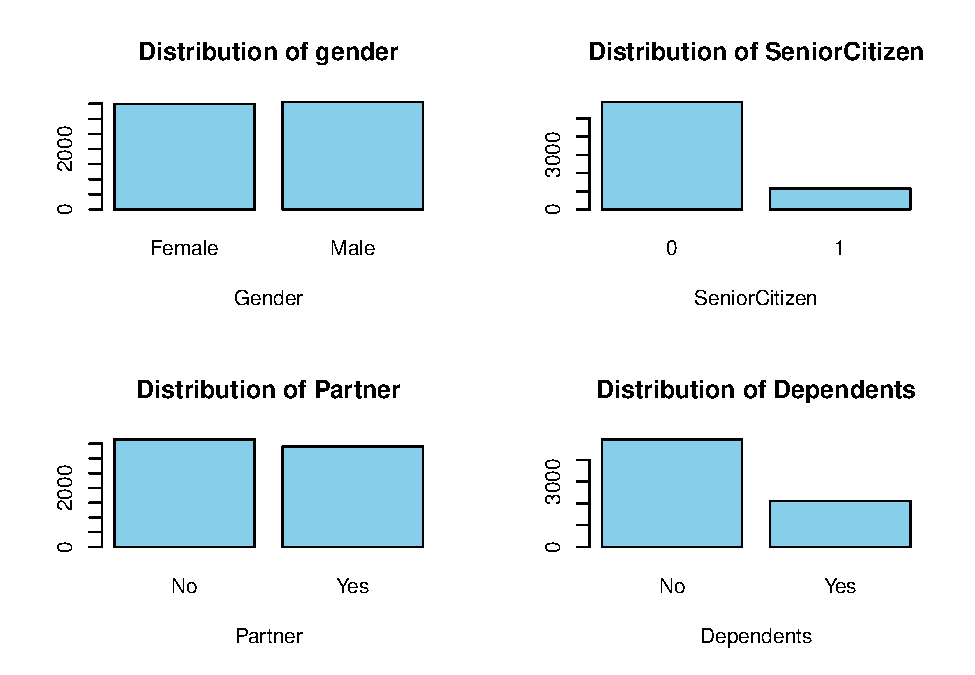
\includegraphics{Assigment2_files/figure-latex/unnamed-chunk-8-1.pdf}

\hypertarget{services-of-the-costumer-data}{%
\subsubsection{\texorpdfstring{\textbf{Services of the costumer
data}}{Services of the costumer data}}\label{services-of-the-costumer-data}}

Services that each customer has signed up for:

\textbf{tenure}

It is a numerical variable that indicates the duration, in months, that
the customer has stayed with the company. We shall explore the
statistics of the variable and look for the \emph{outliers}

\begin{verbatim}
##    Min. 1st Qu.  Median    Mean 3rd Qu.    Max. 
##    0.00    9.00   29.00   32.37   55.00   72.00
\end{verbatim}

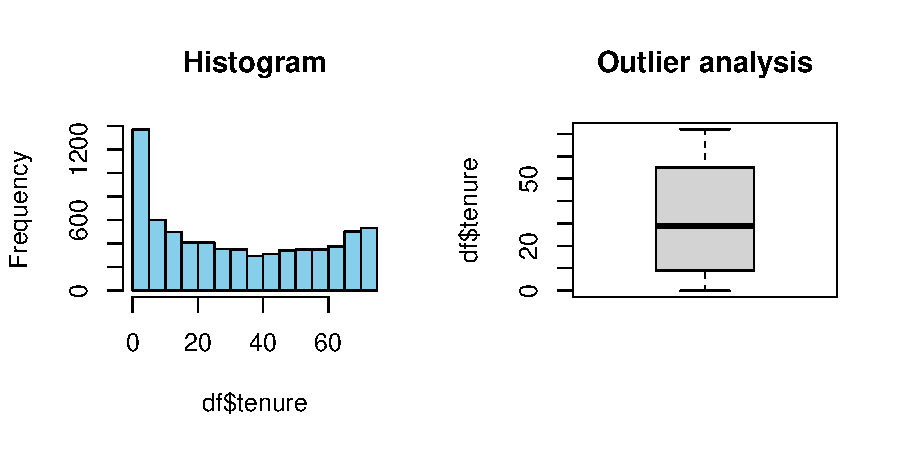
\includegraphics{Assigment2_files/figure-latex/unnamed-chunk-9-1.pdf}

\begin{Shaded}
\begin{Highlighting}[]
\FunctionTok{par}\NormalTok{(}\AttributeTok{mfrow =} \FunctionTok{c}\NormalTok{(}\DecValTok{1}\NormalTok{, }\DecValTok{1}\NormalTok{))}
\NormalTok{sm\_t }\OtherTok{\textless{}{-}} \FunctionTok{summary}\NormalTok{(df}\SpecialCharTok{$}\NormalTok{tenure)}
\NormalTok{iqr\_t }\OtherTok{\textless{}{-}}\NormalTok{ sm\_t[}\StringTok{"3rd Qu."}\NormalTok{] }\SpecialCharTok{{-}}\NormalTok{ sm\_t[}\StringTok{"1st Qu."}\NormalTok{]}
\CommentTok{\# Mild Outliers}
\NormalTok{mild\_ub\_t }\OtherTok{\textless{}{-}}\NormalTok{ sm\_t[}\StringTok{"3rd Qu."}\NormalTok{] }\SpecialCharTok{+} \FloatTok{1.5} \SpecialCharTok{*}\NormalTok{ iqr\_t}
\NormalTok{mild\_lb\_t }\OtherTok{\textless{}{-}}\NormalTok{ sm\_t[}\StringTok{"1st Qu."}\NormalTok{] }\SpecialCharTok{{-}} \FloatTok{1.5} \SpecialCharTok{*}\NormalTok{ iqr\_t}
\FunctionTok{length}\NormalTok{(}\FunctionTok{which}\NormalTok{(df}\SpecialCharTok{$}\NormalTok{tenure }\SpecialCharTok{\textgreater{}}\NormalTok{ mild\_ub\_t }\SpecialCharTok{|}\NormalTok{ df}\SpecialCharTok{$}\NormalTok{tenure }\SpecialCharTok{\textless{}}\NormalTok{ mild\_lb\_t))}
\end{Highlighting}
\end{Shaded}

\begin{verbatim}
## [1] 0
\end{verbatim}

\begin{Shaded}
\begin{Highlighting}[]
\CommentTok{\# number of mild outliers}

\CommentTok{\# Severe Outliers}
\NormalTok{severe\_ub\_t }\OtherTok{\textless{}{-}}\NormalTok{ sm\_t[}\StringTok{"3rd Qu."}\NormalTok{] }\SpecialCharTok{+} \DecValTok{3} \SpecialCharTok{*}\NormalTok{ iqr\_t}
\NormalTok{severe\_lb\_t }\OtherTok{\textless{}{-}}\NormalTok{ sm\_t[}\StringTok{"1st Qu."}\NormalTok{] }\SpecialCharTok{{-}} \DecValTok{3} \SpecialCharTok{*}\NormalTok{ iqr\_t}
\FunctionTok{length}\NormalTok{(}\FunctionTok{which}\NormalTok{(df}\SpecialCharTok{$}\NormalTok{tenure }\SpecialCharTok{\textgreater{}}\NormalTok{ severe\_ub\_t }\SpecialCharTok{|}\NormalTok{ df}\SpecialCharTok{$}\NormalTok{tenure }\SpecialCharTok{\textless{}}\NormalTok{ severe\_lb\_t))}
\end{Highlighting}
\end{Shaded}

\begin{verbatim}
## [1] 0
\end{verbatim}

\begin{Shaded}
\begin{Highlighting}[]
\CommentTok{\# number of severe outliers}
\end{Highlighting}
\end{Shaded}

There are \textbf{no mild nor severe outliers} in Tenure.

\textbf{PhoneService}

It is a binary variable. Levels: Yes/No.~It doesn't contain NA values.

\begin{verbatim}
## [1] 0
\end{verbatim}

\begin{verbatim}
## 
##   No  Yes 
##  682 6361
\end{verbatim}

\textbf{MultipleLines}

Categorical variable with 3 levels, No/No phone service/Yes. It doesn't
contain NA values.

\begin{verbatim}
## [1] 0
\end{verbatim}

\begin{verbatim}
## 
##               No No phone service              Yes 
##             3390              682             2971
\end{verbatim}

Check for inconsistencies:

\begin{itemize}
\tightlist
\item
  It cannot happen that a costumer has not Phoneservice and
  Multiplelines.
\end{itemize}

\begin{verbatim}
##  [1] customerID       gender           SeniorCitizen    Partner         
##  [5] Dependents       tenure           PhoneService     MultipleLines   
##  [9] InternetService  OnlineSecurity   OnlineBackup     DeviceProtection
## [13] TechSupport      StreamingTV      StreamingMovies  Contract        
## [17] PaperlessBilling PaymentMethod    MonthlyCharges   TotalCharges    
## [21] Churn           
## <0 rows> (or 0-length row.names)
\end{verbatim}

\textbf{InternetService}

Categorical variable with 3 levels: DSL/Fiber optic/No.~It doesn't
contain NA values.

\begin{verbatim}
## 
##         DSL Fiber optic          No 
##        2421        3096        1526
\end{verbatim}

\begin{verbatim}
## [1] 0
\end{verbatim}

\textbf{OnlineSecurity}

Categorical variable with 3 levels: No/No internet service/Yes. It
doesn't contain NA values.

\begin{verbatim}
## 
##                  No No internet service                 Yes 
##                3498                1526                2019
\end{verbatim}

\begin{verbatim}
## [1] 0
\end{verbatim}

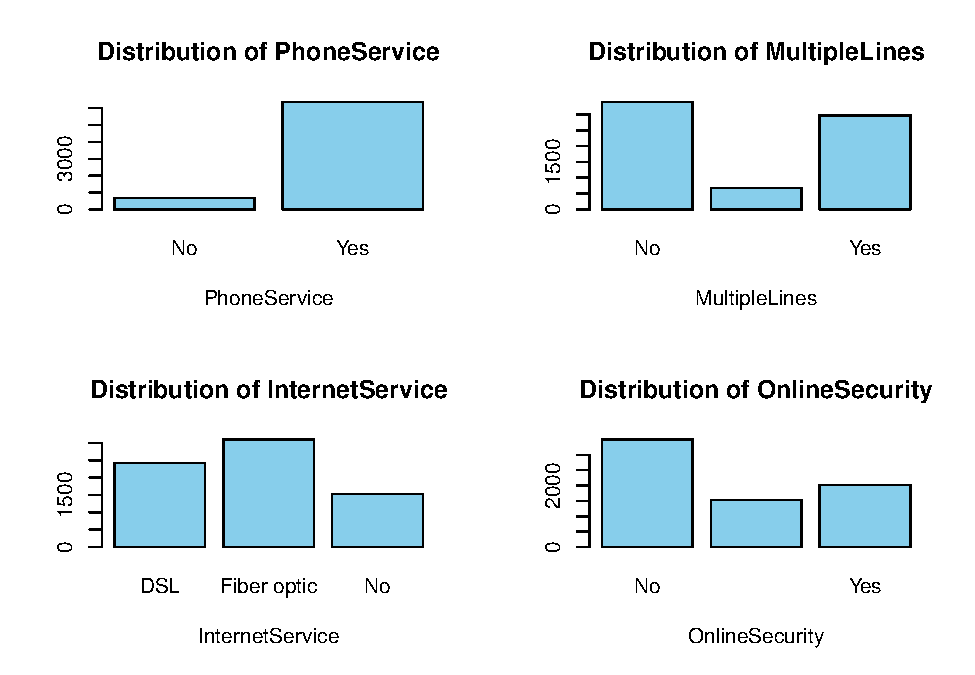
\includegraphics{Assigment2_files/figure-latex/unnamed-chunk-16-1.pdf}

Check consistency

\begin{Shaded}
\begin{Highlighting}[]
\FunctionTok{sum}\NormalTok{(df}\SpecialCharTok{$}\NormalTok{InternetService }\SpecialCharTok{==} \StringTok{"No"}\NormalTok{)}
\end{Highlighting}
\end{Shaded}

\begin{verbatim}
## [1] 1526
\end{verbatim}

\begin{Shaded}
\begin{Highlighting}[]
\FunctionTok{sum}\NormalTok{(df}\SpecialCharTok{$}\NormalTok{OnlineSecurity }\SpecialCharTok{==} \StringTok{"No internet service"}\NormalTok{)}
\end{Highlighting}
\end{Shaded}

\begin{verbatim}
## [1] 1526
\end{verbatim}

\begin{Shaded}
\begin{Highlighting}[]
\FunctionTok{nrow}\NormalTok{(}\FunctionTok{subset}\NormalTok{(df, InternetService }\SpecialCharTok{==} \StringTok{"No"} \SpecialCharTok{\&}\NormalTok{ OnlineSecurity }\SpecialCharTok{==} \StringTok{"No internet service"}\NormalTok{))}
\end{Highlighting}
\end{Shaded}

\begin{verbatim}
## [1] 1526
\end{verbatim}

\textbf{OnlineBackup}

Categorical variable with 3 levels: No/No internet service/Yes. It
doesn't contain NA values.

\begin{verbatim}
## 
##                  No No internet service                 Yes 
##                3088                1526                2429
\end{verbatim}

\begin{verbatim}
## [1] 0
\end{verbatim}

\begin{Shaded}
\begin{Highlighting}[]
\CommentTok{\# Check concistency}
\FunctionTok{sum}\NormalTok{(df}\SpecialCharTok{$}\NormalTok{OnlineBackup }\SpecialCharTok{==} \StringTok{"No internet service"}\NormalTok{) }\CommentTok{\#1526}
\end{Highlighting}
\end{Shaded}

\begin{verbatim}
## [1] 1526
\end{verbatim}

\begin{Shaded}
\begin{Highlighting}[]
\FunctionTok{sum}\NormalTok{(df}\SpecialCharTok{$}\NormalTok{OnlineSecurity }\SpecialCharTok{==} \StringTok{"No internet service"}\NormalTok{) }\CommentTok{\#1526}
\end{Highlighting}
\end{Shaded}

\begin{verbatim}
## [1] 1526
\end{verbatim}

\textbf{DeviceProtection} Categorical variable with 3 levels: No/No
internet service/Yes. It doesn't contain NA values.

\begin{verbatim}
## 
##                  No No internet service                 Yes 
##                3095                1526                2422
\end{verbatim}

\begin{verbatim}
## [1] 0
\end{verbatim}

\begin{Shaded}
\begin{Highlighting}[]
\CommentTok{\# Check consistency}
\FunctionTok{sum}\NormalTok{(df}\SpecialCharTok{$}\NormalTok{OnlineSecurity }\SpecialCharTok{==} \StringTok{"No internet service"}\NormalTok{) }\CommentTok{\#1526}
\end{Highlighting}
\end{Shaded}

\begin{verbatim}
## [1] 1526
\end{verbatim}

\begin{Shaded}
\begin{Highlighting}[]
\FunctionTok{sum}\NormalTok{(df}\SpecialCharTok{$}\NormalTok{DeviceProtection }\SpecialCharTok{==} \StringTok{"No internet service"}\NormalTok{) }\CommentTok{\#1526}
\end{Highlighting}
\end{Shaded}

\begin{verbatim}
## [1] 1526
\end{verbatim}

\textbf{TechSupport}

Categorical variable with 3 levels: No/No internet service/Yes. It
doesn't contain NA values.

\begin{verbatim}
## 
##                  No No internet service                 Yes 
##                3473                1526                2044
\end{verbatim}

\begin{verbatim}
## [1] 0
\end{verbatim}

\begin{Shaded}
\begin{Highlighting}[]
\CommentTok{\#Check consistency}
\FunctionTok{sum}\NormalTok{(df}\SpecialCharTok{$}\NormalTok{DeviceProtection }\SpecialCharTok{==} \StringTok{"No internet service"}\NormalTok{) }\CommentTok{\#1526}
\end{Highlighting}
\end{Shaded}

\begin{verbatim}
## [1] 1526
\end{verbatim}

\begin{Shaded}
\begin{Highlighting}[]
\FunctionTok{sum}\NormalTok{(df}\SpecialCharTok{$}\NormalTok{TechSupport }\SpecialCharTok{==} \StringTok{"No internet service"}\NormalTok{) }\CommentTok{\#1526}
\end{Highlighting}
\end{Shaded}

\begin{verbatim}
## [1] 1526
\end{verbatim}

\textbf{StreamingTV} Categorical variable with 3 levels: No/No internet
service/Yes. It doesn't contain NA values.

\begin{verbatim}
## 
##                  No No internet service                 Yes 
##                2810                1526                2707
\end{verbatim}

\begin{verbatim}
## [1] 0
\end{verbatim}

\begin{Shaded}
\begin{Highlighting}[]
\CommentTok{\#Check consistency}
\FunctionTok{sum}\NormalTok{(df}\SpecialCharTok{$}\NormalTok{TechSupport }\SpecialCharTok{==} \StringTok{"No internet service"}\NormalTok{) }\CommentTok{\#1526}
\end{Highlighting}
\end{Shaded}

\begin{verbatim}
## [1] 1526
\end{verbatim}

\begin{Shaded}
\begin{Highlighting}[]
\FunctionTok{sum}\NormalTok{(df}\SpecialCharTok{$}\NormalTok{StreamingTV }\SpecialCharTok{==} \StringTok{"No internet service"}\NormalTok{) }\CommentTok{\#1526}
\end{Highlighting}
\end{Shaded}

\begin{verbatim}
## [1] 1526
\end{verbatim}

\textbf{StreamingMovies}

Categorical variable with 3 levels: No/No internet service/Yes. It
doesn't contain NA values.

\begin{verbatim}
## 
##                  No No internet service                 Yes 
##                2785                1526                2732
\end{verbatim}

\begin{verbatim}
## [1] 0
\end{verbatim}

\begin{Shaded}
\begin{Highlighting}[]
\CommentTok{\#Check consistency}
\FunctionTok{sum}\NormalTok{(df}\SpecialCharTok{$}\NormalTok{StreamingTV }\SpecialCharTok{==} \StringTok{"No internet service"}\NormalTok{) }\CommentTok{\#1526}
\end{Highlighting}
\end{Shaded}

\begin{verbatim}
## [1] 1526
\end{verbatim}

\begin{Shaded}
\begin{Highlighting}[]
\FunctionTok{sum}\NormalTok{(df}\SpecialCharTok{$}\NormalTok{StreamingMovies }\SpecialCharTok{==} \StringTok{"No internet service"}\NormalTok{) }\CommentTok{\#1526}
\end{Highlighting}
\end{Shaded}

\begin{verbatim}
## [1] 1526
\end{verbatim}

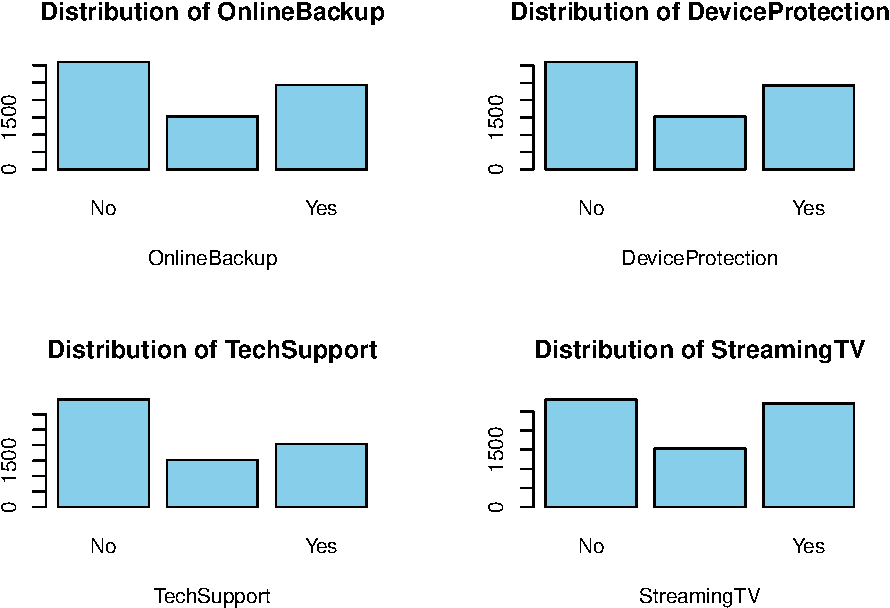
\includegraphics{Assigment2_files/figure-latex/unnamed-chunk-28-1.pdf}
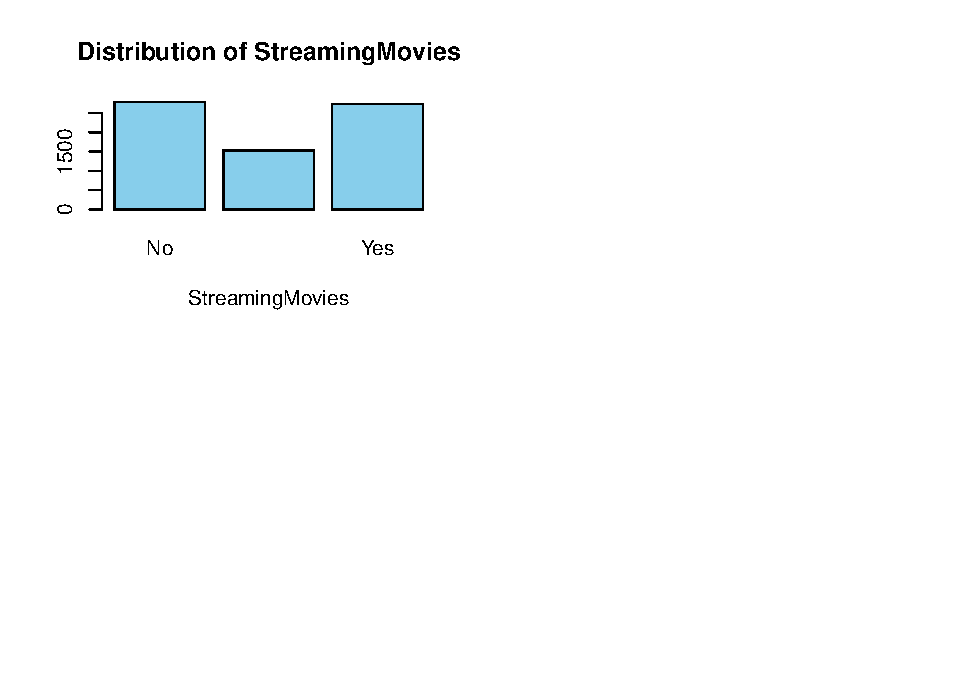
\includegraphics{Assigment2_files/figure-latex/unnamed-chunk-28-2.pdf}

\hypertarget{customer-account-data}{%
\subsubsection{Customer account data}\label{customer-account-data}}

\textbf{Contract} Categorical variable with 3 levels: Month-to-month/One
year/Two year. It doesn't contain NA values.

\begin{verbatim}
## 
## Month-to-month       One year       Two year 
##           3875           1473           1695
\end{verbatim}

\begin{verbatim}
## [1] 0
\end{verbatim}

\textbf{PaperlessBilling} It is a binary variable. Levels: No/Yes. It
doesn't contain NA values.

\begin{Shaded}
\begin{Highlighting}[]
\FunctionTok{table}\NormalTok{(df}\SpecialCharTok{$}\NormalTok{PaperlessBilling)}
\end{Highlighting}
\end{Shaded}

\begin{verbatim}
## 
##   No  Yes 
## 2872 4171
\end{verbatim}

\begin{Shaded}
\begin{Highlighting}[]
\FunctionTok{sum}\NormalTok{(}\FunctionTok{is.na}\NormalTok{(df}\SpecialCharTok{$}\NormalTok{PaperlessBilling))}
\end{Highlighting}
\end{Shaded}

\begin{verbatim}
## [1] 0
\end{verbatim}

\textbf{PaymentMethod} Categorical variable with 4 levels: Bank transfer
(automatic)/Credit card (automatic)/Electronic check/Mailed check. It
doesn't contain NA values.

\begin{Shaded}
\begin{Highlighting}[]
\FunctionTok{table}\NormalTok{(df}\SpecialCharTok{$}\NormalTok{PaymentMethod)}
\end{Highlighting}
\end{Shaded}

\begin{verbatim}
## 
## Bank transfer (automatic)   Credit card (automatic)          Electronic check 
##                      1544                      1522                      2365 
##              Mailed check 
##                      1612
\end{verbatim}

\begin{Shaded}
\begin{Highlighting}[]
\FunctionTok{sum}\NormalTok{(}\FunctionTok{is.na}\NormalTok{(df}\SpecialCharTok{$}\NormalTok{PaymentMethod))}
\end{Highlighting}
\end{Shaded}

\begin{verbatim}
## [1] 0
\end{verbatim}

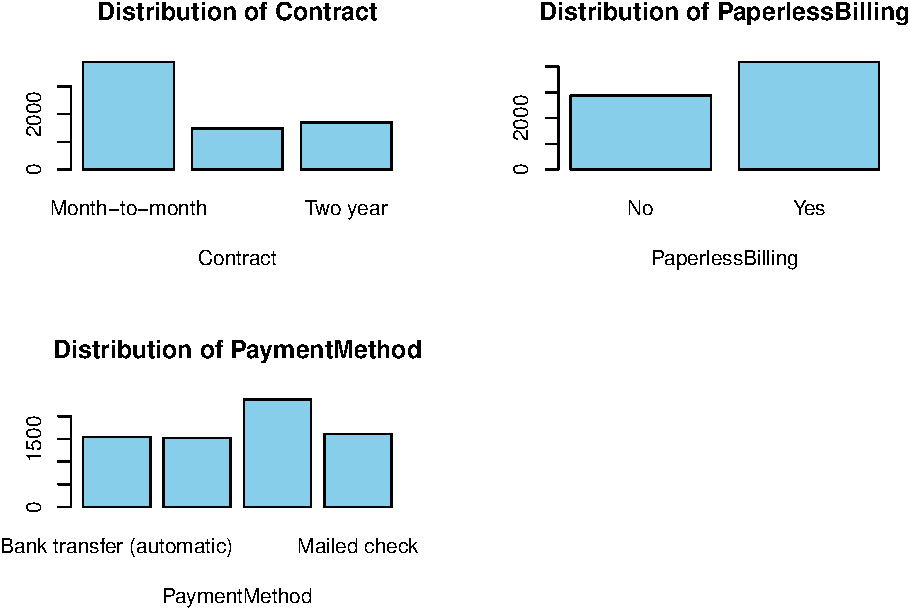
\includegraphics{Assigment2_files/figure-latex/unnamed-chunk-32-1.pdf}

\textbf{MonthlyCharges}

It is a numerical variable. It doesn't contain NA values.

\begin{verbatim}
##    Min. 1st Qu.  Median    Mean 3rd Qu.    Max. 
##   18.25   35.50   70.35   64.76   89.85  118.75
\end{verbatim}

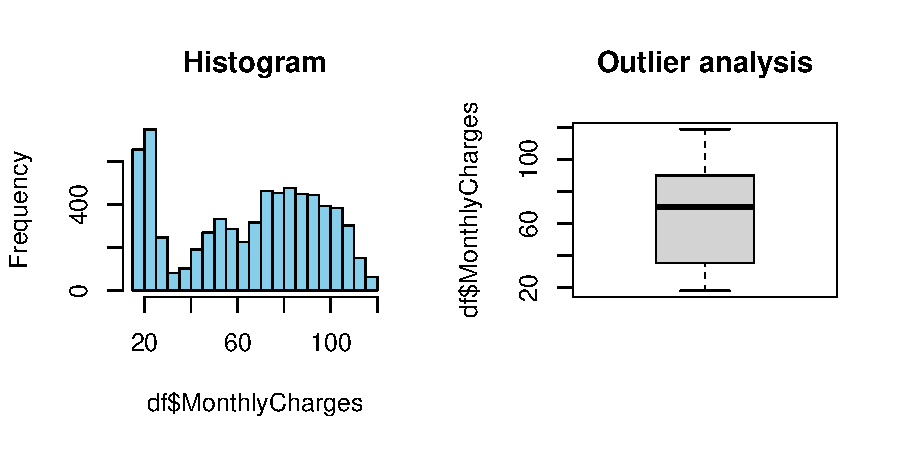
\includegraphics{Assigment2_files/figure-latex/unnamed-chunk-33-1.pdf}

\begin{verbatim}
## [1] 0
\end{verbatim}

Let's look for \emph{outliers}.

\begin{Shaded}
\begin{Highlighting}[]
\NormalTok{sm }\OtherTok{\textless{}{-}} \FunctionTok{summary}\NormalTok{(df}\SpecialCharTok{$}\NormalTok{MonthlyCharges)}
\NormalTok{iqr }\OtherTok{\textless{}{-}}\NormalTok{ sm[}\StringTok{"3rd Qu."}\NormalTok{] }\SpecialCharTok{{-}}\NormalTok{ sm[}\StringTok{"1st Qu."}\NormalTok{]}
\CommentTok{\# Mild Outliers}
\NormalTok{mild\_ub }\OtherTok{\textless{}{-}}\NormalTok{ sm[}\StringTok{"3rd Qu."}\NormalTok{] }\SpecialCharTok{+} \FloatTok{1.5} \SpecialCharTok{*}\NormalTok{ iqr}
\NormalTok{mild\_lb }\OtherTok{\textless{}{-}}\NormalTok{ sm[}\StringTok{"1st Qu."}\NormalTok{] }\SpecialCharTok{{-}} \FloatTok{1.5} \SpecialCharTok{*}\NormalTok{ iqr}
\FunctionTok{length}\NormalTok{(}\FunctionTok{which}\NormalTok{(df}\SpecialCharTok{$}\NormalTok{MonthlyCharges }\SpecialCharTok{\textgreater{}}\NormalTok{ mild\_ub }\SpecialCharTok{|}\NormalTok{ df}\SpecialCharTok{$}\NormalTok{MonthlyCharges }\SpecialCharTok{\textless{}}\NormalTok{ mild\_lb)) }
\end{Highlighting}
\end{Shaded}

\begin{verbatim}
## [1] 0
\end{verbatim}

\begin{Shaded}
\begin{Highlighting}[]
\CommentTok{\# Severe Outliers}
\NormalTok{severe\_ub }\OtherTok{\textless{}{-}}\NormalTok{ sm[}\StringTok{"3rd Qu."}\NormalTok{] }\SpecialCharTok{+} \DecValTok{3} \SpecialCharTok{*}\NormalTok{ iqr}
\NormalTok{severe\_lb }\OtherTok{\textless{}{-}}\NormalTok{ sm[}\StringTok{"1st Qu."}\NormalTok{] }\SpecialCharTok{{-}} \DecValTok{3} \SpecialCharTok{*}\NormalTok{ iqr}
\FunctionTok{length}\NormalTok{(}\FunctionTok{which}\NormalTok{(df}\SpecialCharTok{$}\NormalTok{MonthlyCharges }\SpecialCharTok{\textgreater{}}\NormalTok{ severe\_ub }\SpecialCharTok{|}\NormalTok{ df}\SpecialCharTok{$}\NormalTok{MonthlyCharges }\SpecialCharTok{\textless{}}\NormalTok{ severe\_lb)) }
\end{Highlighting}
\end{Shaded}

\begin{verbatim}
## [1] 0
\end{verbatim}

There are no mild nor severe outliers in MonthlyCharges.

\textbf{TotalCharges}

It is a numerical variable. It does contain 11 NA values.

\begin{verbatim}
##    Min. 1st Qu.  Median    Mean 3rd Qu.    Max.    NA's 
##    18.8   401.4  1397.5  2283.3  3794.7  8684.8      11
\end{verbatim}

\begin{verbatim}
## [1] 11
\end{verbatim}

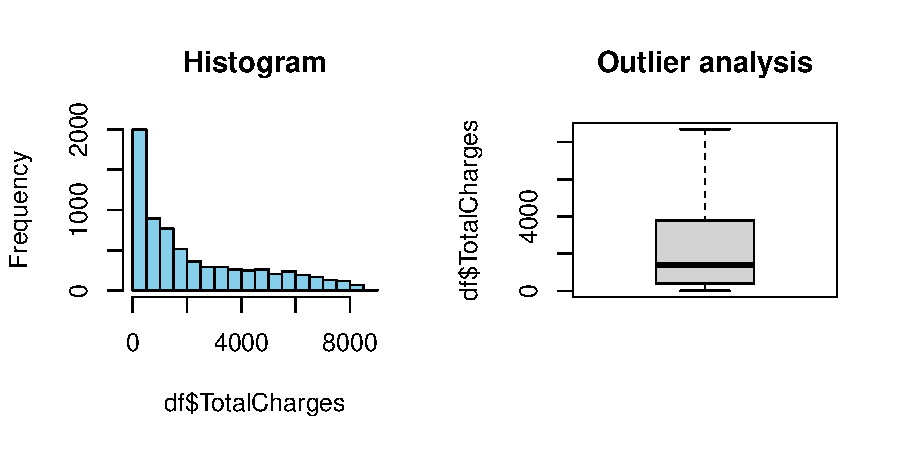
\includegraphics{Assigment2_files/figure-latex/unnamed-chunk-35-1.pdf}

\begin{verbatim}
## [1] 11
\end{verbatim}

Let's look for \emph{outliers}.

\begin{Shaded}
\begin{Highlighting}[]
\NormalTok{sm }\OtherTok{\textless{}{-}} \FunctionTok{summary}\NormalTok{(df}\SpecialCharTok{$}\NormalTok{TotalCharges)}
\NormalTok{iqr }\OtherTok{\textless{}{-}}\NormalTok{ sm[}\StringTok{"3rd Qu."}\NormalTok{] }\SpecialCharTok{{-}}\NormalTok{ sm[}\StringTok{"1st Qu."}\NormalTok{]}
\CommentTok{\# Mild Outliers}
\NormalTok{mild\_ub }\OtherTok{\textless{}{-}}\NormalTok{ sm[}\StringTok{"3rd Qu."}\NormalTok{] }\SpecialCharTok{+} \FloatTok{1.5} \SpecialCharTok{*}\NormalTok{ iqr}
\NormalTok{mild\_lb }\OtherTok{\textless{}{-}}\NormalTok{ sm[}\StringTok{"1st Qu."}\NormalTok{] }\SpecialCharTok{{-}} \FloatTok{1.5} \SpecialCharTok{*}\NormalTok{ iqr}
\FunctionTok{length}\NormalTok{(}\FunctionTok{which}\NormalTok{(df}\SpecialCharTok{$}\NormalTok{TotalCharges }\SpecialCharTok{\textgreater{}}\NormalTok{ mild\_ub }\SpecialCharTok{|}\NormalTok{ df}\SpecialCharTok{$}\NormalTok{TotalCharges }\SpecialCharTok{\textless{}}\NormalTok{ mild\_lb))}
\end{Highlighting}
\end{Shaded}

\begin{verbatim}
## [1] 0
\end{verbatim}

\begin{Shaded}
\begin{Highlighting}[]
\CommentTok{\# Severe Outliers}
\NormalTok{severe\_ub }\OtherTok{\textless{}{-}}\NormalTok{ sm[}\StringTok{"3rd Qu."}\NormalTok{] }\SpecialCharTok{+} \DecValTok{3} \SpecialCharTok{*}\NormalTok{ iqr}
\NormalTok{severe\_lb }\OtherTok{\textless{}{-}}\NormalTok{ sm[}\StringTok{"1st Qu."}\NormalTok{] }\SpecialCharTok{{-}} \DecValTok{3} \SpecialCharTok{*}\NormalTok{ iqr}
\FunctionTok{length}\NormalTok{(}\FunctionTok{which}\NormalTok{(df}\SpecialCharTok{$}\NormalTok{TotalCharges }\SpecialCharTok{\textgreater{}}\NormalTok{ severe\_ub }\SpecialCharTok{|}\NormalTok{ df}\SpecialCharTok{$}\NormalTok{TotalCharges }\SpecialCharTok{\textless{}}\NormalTok{ severe\_lb))}
\end{Highlighting}
\end{Shaded}

\begin{verbatim}
## [1] 0
\end{verbatim}

There are no mild nor severe outliers.

\hypertarget{target-variable}{%
\subsubsection{Target variable:}\label{target-variable}}

\textbf{Churn} It is the target variable. It is binary, describes
whether the customer churned or not (Yes or No).

\begin{Shaded}
\begin{Highlighting}[]
\FunctionTok{table}\NormalTok{(df}\SpecialCharTok{$}\NormalTok{Churn)}
\end{Highlighting}
\end{Shaded}

\begin{verbatim}
## 
##   No  Yes 
## 5174 1869
\end{verbatim}

\begin{Shaded}
\begin{Highlighting}[]
\FunctionTok{prop.table}\NormalTok{(}\FunctionTok{table}\NormalTok{(df}\SpecialCharTok{$}\NormalTok{Churn))}
\end{Highlighting}
\end{Shaded}

\begin{verbatim}
## 
##        No       Yes 
## 0.7346301 0.2653699
\end{verbatim}

\begin{Shaded}
\begin{Highlighting}[]
\FunctionTok{barplot}\NormalTok{(}\FunctionTok{table}\NormalTok{(df}\SpecialCharTok{$}\NormalTok{Churn), }\AttributeTok{col=}\StringTok{"skyblue"}\NormalTok{)}
\end{Highlighting}
\end{Shaded}

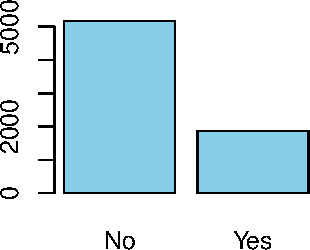
\includegraphics{Assigment2_files/figure-latex/unnamed-chunk-37-1.pdf}

\begin{Shaded}
\begin{Highlighting}[]
\FunctionTok{sum}\NormalTok{(}\FunctionTok{is.na}\NormalTok{(df}\SpecialCharTok{$}\NormalTok{Churn))}
\end{Highlighting}
\end{Shaded}

\begin{verbatim}
## [1] 0
\end{verbatim}

\hypertarget{data-preprocessing}{%
\section{Data preprocessing}\label{data-preprocessing}}

\hypertarget{recode-variables-into-correct-type}{%
\subsubsection{Recode variables into correct
type}\label{recode-variables-into-correct-type}}

We shall reconvert the type of certain variables that are encoded with
wrong type. First, we convert the character variables (except the ID)
into factors.

\begin{Shaded}
\begin{Highlighting}[]
\NormalTok{char\_cols }\OtherTok{\textless{}{-}} \FunctionTok{which}\NormalTok{(}\FunctionTok{sapply}\NormalTok{(df, is.character))}
\NormalTok{df[, char\_cols[}\SpecialCharTok{{-}}\DecValTok{1}\NormalTok{]]}\OtherTok{\textless{}{-}} \FunctionTok{lapply}\NormalTok{(df[, char\_cols[}\SpecialCharTok{{-}}\DecValTok{1}\NormalTok{]], as.factor) }
\end{Highlighting}
\end{Shaded}

Also, we convert the numerical variable SeniorCitizen into a factor.

\begin{Shaded}
\begin{Highlighting}[]
\NormalTok{df}\SpecialCharTok{$}\NormalTok{SeniorCitizen}\OtherTok{\textless{}{-}} \FunctionTok{factor}\NormalTok{(df}\SpecialCharTok{$}\NormalTok{SeniorCitizen)}
\end{Highlighting}
\end{Shaded}

\hypertarget{data-imputation}{%
\subsubsection{Data imputation}\label{data-imputation}}

\begin{verbatim}
##  customerID        gender        SeniorCitizen    Partner       
##  Mode :logical   Mode :logical   Mode :logical   Mode :logical  
##  FALSE:7043      FALSE:7043      FALSE:7043      FALSE:7043     
##                                                                 
##  Dependents        tenure        PhoneService    MultipleLines  
##  Mode :logical   Mode :logical   Mode :logical   Mode :logical  
##  FALSE:7043      FALSE:7043      FALSE:7043      FALSE:7043     
##                                                                 
##  InternetService OnlineSecurity  OnlineBackup    DeviceProtection
##  Mode :logical   Mode :logical   Mode :logical   Mode :logical   
##  FALSE:7043      FALSE:7043      FALSE:7043      FALSE:7043      
##                                                                  
##  TechSupport     StreamingTV     StreamingMovies  Contract      
##  Mode :logical   Mode :logical   Mode :logical   Mode :logical  
##  FALSE:7043      FALSE:7043      FALSE:7043      FALSE:7043     
##                                                                 
##  PaperlessBilling PaymentMethod   MonthlyCharges  TotalCharges   
##  Mode :logical    Mode :logical   Mode :logical   Mode :logical  
##  FALSE:7043       FALSE:7043      FALSE:7043      FALSE:7032     
##                                                   TRUE :11       
##    Churn        
##  Mode :logical  
##  FALSE:7043     
## 
\end{verbatim}

Only the variable TotalCharges has NA's.

The missing data corresponds to the individuals that have not payed yet
the charges of the current month, we can guess that are new clients of
the company.

Duplicate values: no

\begin{Shaded}
\begin{Highlighting}[]
\FunctionTok{length}\NormalTok{(}\FunctionTok{unique}\NormalTok{(df}\SpecialCharTok{$}\NormalTok{customerID))}
\end{Highlighting}
\end{Shaded}

\begin{verbatim}
## [1] 7043
\end{verbatim}

These NA exist because the costumer hasn't payed yet that month (tenure
is 0). We convert these NA to 0.

\begin{Shaded}
\begin{Highlighting}[]
\NormalTok{ll }\OtherTok{\textless{}{-}} \FunctionTok{which}\NormalTok{(}\FunctionTok{is.na}\NormalTok{(df}\SpecialCharTok{$}\NormalTok{TotalCharges))}
\NormalTok{df[ll,}\StringTok{"TotalCharges"}\NormalTok{] }\OtherTok{\textless{}{-}} \DecValTok{0}
\end{Highlighting}
\end{Shaded}

\hypertarget{correlation-between-categorical}{%
\subsubsection{Correlation between
categorical}\label{correlation-between-categorical}}

The categorical variables MultipleLines and PhoneService are 100\%
correlated. We might have multicollinearity between these two variables.

\begin{Shaded}
\begin{Highlighting}[]
\NormalTok{contingency\_table}\OtherTok{\textless{}{-}}\FunctionTok{table}\NormalTok{(df}\SpecialCharTok{$}\NormalTok{MultipleLines,df}\SpecialCharTok{$}\NormalTok{PhoneService)}
\FunctionTok{sqrt}\NormalTok{(}\FunctionTok{chisq.test}\NormalTok{(contingency\_table)}\SpecialCharTok{$}\NormalTok{statistic }\SpecialCharTok{/}\NormalTok{ (}\FunctionTok{sum}\NormalTok{(contingency\_table) }\SpecialCharTok{*}\NormalTok{ (}\FunctionTok{min}\NormalTok{(}\FunctionTok{dim}\NormalTok{(contingency\_table)) }\SpecialCharTok{{-}} \DecValTok{1}\NormalTok{)))}
\end{Highlighting}
\end{Shaded}

\begin{verbatim}
## X-squared 
##         1
\end{verbatim}

\hypertarget{profiling}{%
\subsubsection{Profiling}\label{profiling}}

\begin{Shaded}
\begin{Highlighting}[]
\NormalTok{res.cat}\OtherTok{=}\FunctionTok{catdes}\NormalTok{(df, }\DecValTok{21}\NormalTok{)}
\NormalTok{res.cat}\SpecialCharTok{$}\NormalTok{test.chi2}
\end{Highlighting}
\end{Shaded}

\begin{verbatim}
##                        p.value df
## Contract         5.863038e-258  2
## OnlineSecurity   2.661150e-185  2
## TechSupport      1.443084e-180  2
## InternetService  9.571788e-160  2
## PaymentMethod    3.682355e-140  3
## OnlineBackup     2.079759e-131  2
## DeviceProtection 5.505219e-122  2
## StreamingMovies   2.667757e-82  2
## StreamingTV       5.528994e-82  2
## PaperlessBilling  2.614597e-58  1
## Dependents        3.276083e-43  1
## SeniorCitizen     9.477904e-37  1
## Partner           1.519037e-36  1
## MultipleLines     3.464383e-03  2
\end{verbatim}

\begin{Shaded}
\begin{Highlighting}[]
\FunctionTok{lapply}\NormalTok{(res.cat}\SpecialCharTok{$}\NormalTok{category, head, }\AttributeTok{n =} \DecValTok{5}\NormalTok{)}
\end{Highlighting}
\end{Shaded}

\begin{verbatim}
## $No
##                                       Cla/Mod  Mod/Cla   Global       p.value
## Contract=Two year                    97.16814 31.83224 24.06645 3.588830e-187
## StreamingMovies=No internet service  92.59502 27.30963 21.66690  6.584621e-98
## StreamingTV=No internet service      92.59502 27.30963 21.66690  6.584621e-98
## TechSupport=No internet service      92.59502 27.30963 21.66690  6.584621e-98
## DeviceProtection=No internet service 92.59502 27.30963 21.66690  6.584621e-98
##                                        v.test
## Contract=Two year                    29.17894
## StreamingMovies=No internet service  20.99981
## StreamingTV=No internet service      20.99981
## TechSupport=No internet service      20.99981
## DeviceProtection=No internet service 20.99981
## 
## $Yes
##                                 Cla/Mod  Mod/Cla   Global       p.value
## Contract=Month-to-month        42.70968 88.55003 55.01917 3.620915e-283
## OnlineSecurity=No              41.76672 78.17014 49.66634 6.171504e-190
## TechSupport=No                 41.63547 77.36758 49.31137 1.899538e-183
## InternetService=Fiber optic    41.89276 69.39540 43.95854 2.289126e-148
## PaymentMethod=Electronic check 45.28541 57.30337 33.57944 1.790860e-136
##                                  v.test
## Contract=Month-to-month        35.95931
## OnlineSecurity=No              29.39603
## TechSupport=No                 28.88395
## InternetService=Fiber optic    25.94114
## PaymentMethod=Electronic check 24.86476
\end{verbatim}

\begin{Shaded}
\begin{Highlighting}[]
\FunctionTok{lapply}\NormalTok{(res.cat}\SpecialCharTok{$}\NormalTok{category, tail, }\AttributeTok{n =} \DecValTok{5}\NormalTok{)}
\end{Highlighting}
\end{Shaded}

\begin{verbatim}
## $No
##                                 Cla/Mod  Mod/Cla   Global       p.value
## PaymentMethod=Electronic check 54.71459 25.00966 33.57944 1.790860e-136
## InternetService=Fiber optic    58.10724 34.77000 43.95854 2.289126e-148
## TechSupport=No                 58.36453 39.17665 49.31137 1.899538e-183
## OnlineSecurity=No              58.23328 39.36993 49.66634 6.171504e-190
## Contract=Month-to-month        57.29032 42.90684 55.01917 3.620915e-283
##                                   v.test
## PaymentMethod=Electronic check -24.86476
## InternetService=Fiber optic    -25.94114
## TechSupport=No                 -28.88395
## OnlineSecurity=No              -29.39603
## Contract=Month-to-month        -35.95931
## 
## $Yes
##                                       Cla/Mod  Mod/Cla   Global       p.value
## DeviceProtection=No internet service 7.404980 6.046014 21.66690  6.584621e-98
## OnlineBackup=No internet service     7.404980 6.046014 21.66690  6.584621e-98
## OnlineSecurity=No internet service   7.404980 6.046014 21.66690  6.584621e-98
## InternetService=No                   7.404980 6.046014 21.66690  6.584621e-98
## Contract=Two year                    2.831858 2.568218 24.06645 3.588830e-187
##                                         v.test
## DeviceProtection=No internet service -20.99981
## OnlineBackup=No internet service     -20.99981
## OnlineSecurity=No internet service   -20.99981
## InternetService=No                   -20.99981
## Contract=Two year                    -29.17894
\end{verbatim}

\begin{Shaded}
\begin{Highlighting}[]
\NormalTok{res.cat}\SpecialCharTok{$}\NormalTok{quanti.var}
\end{Highlighting}
\end{Shaded}

\begin{verbatim}
##                      Eta2       P-value
## tenure         0.12406504 7.999058e-205
## TotalCharges   0.03933251  2.127212e-63
## MonthlyCharges 0.03738671  2.706646e-60
\end{verbatim}

Regarding to the results of the test \(Chi^2\) all correlations with the
variables are significant since the \(p-value\) is less than 0,05. Since
the response variable is binary, we have different results for each
answer and also for all outcomes of the categorical parameters.

The parameters that have a higher positive relation with the costumers
that don't churn are the ones that have a negative relation when the
response variable is ``Yes''. In the same vein, we can observe that the
parameters that have a negative relation with the costumers that churn
are ``OnlineSecurity'' and ``TechSupport'' when the answer is ``No'',
the same parameters that have a positive relation when the costumers
churn. We can see that the target answer ``Yes'' and ``No'' have an
approximate opposite correlations with the explanatory variables.

\hypertarget{modelling}{%
\subsection{Modelling}\label{modelling}}

\hypertarget{data-transformations}{%
\subsubsection{Data transformations:}\label{data-transformations}}

Recall that the following variables:

\begin{itemize}
\item OnlineSecurity
\item OnlineBackup
\item DeviceProtection
\item TechSupport
\item StreamingTV
\item StreamingMovies
\end{itemize}

are categorical variables with 3 levels: No/No internet service/Yes.

We observe that they contain ``No internet service'' as a response. We
have a variable called \emph{InternetService} that is a categorical
variable with 3 levels: DSL/Fiber optic/No.~Whenever
\emph{InternetService}=``No'' implies -\textgreater{} var=``No internet
service''. Therefore we decided to transform the level ``No internet
service'' into ``No'' in the 6 variables above since this variable will
specify.

\begin{Shaded}
\begin{Highlighting}[]
\NormalTok{df}\SpecialCharTok{$}\NormalTok{OnlineSecurity[df}\SpecialCharTok{$}\NormalTok{OnlineSecurity}\SpecialCharTok{==}\StringTok{"No internet service"}\NormalTok{] }\OtherTok{\textless{}{-}} \StringTok{"No"}
\NormalTok{df}\SpecialCharTok{$}\NormalTok{OnlineBackup[df}\SpecialCharTok{$}\NormalTok{OnlineBackup}\SpecialCharTok{==}\StringTok{"No internet service"}\NormalTok{] }\OtherTok{\textless{}{-}} \StringTok{"No"}
\NormalTok{df}\SpecialCharTok{$}\NormalTok{DeviceProtection[df}\SpecialCharTok{$}\NormalTok{DeviceProtection}\SpecialCharTok{==}\StringTok{"No internet service"}\NormalTok{] }\OtherTok{\textless{}{-}} \StringTok{"No"}
\NormalTok{df}\SpecialCharTok{$}\NormalTok{TechSupport[df}\SpecialCharTok{$}\NormalTok{TechSupport}\SpecialCharTok{==}\StringTok{"No internet service"}\NormalTok{] }\OtherTok{\textless{}{-}} \StringTok{"No"}
\NormalTok{df}\SpecialCharTok{$}\NormalTok{StreamingTV[df}\SpecialCharTok{$}\NormalTok{StreamingTV}\SpecialCharTok{==}\StringTok{"No internet service"}\NormalTok{] }\OtherTok{\textless{}{-}} \StringTok{"No"}
\NormalTok{df}\SpecialCharTok{$}\NormalTok{StreamingMovies[df}\SpecialCharTok{$}\NormalTok{StreamingMovies}\SpecialCharTok{==}\StringTok{"No internet service"}\NormalTok{] }\OtherTok{\textless{}{-}} \StringTok{"No"}
\end{Highlighting}
\end{Shaded}

We saw that \emph{MultipleLines} is 100\% related with
\emph{PhoneService}. The reason is similar as the previous parameters:
one answer of \emph{MultipleLines} is ``No phone service''. We set this
answer to ``No'' since we don't lose the information because it is
contained inside the parameter \emph{PhoneService}.

\begin{Shaded}
\begin{Highlighting}[]
\NormalTok{df}\SpecialCharTok{$}\NormalTok{MultipleLines[df}\SpecialCharTok{$}\NormalTok{MultipleLines}\SpecialCharTok{==}\StringTok{"No phone service"}\NormalTok{] }\OtherTok{\textless{}{-}} \StringTok{"No"}
\end{Highlighting}
\end{Shaded}

\hypertarget{modelling-1}{%
\subsubsection{Modelling:}\label{modelling-1}}

\begin{Shaded}
\begin{Highlighting}[]
\FunctionTok{set.seed}\NormalTok{(}\DecValTok{1234}\NormalTok{)}
\NormalTok{m }\OtherTok{\textless{}{-}} \FunctionTok{floor}\NormalTok{(}\FloatTok{0.7}\SpecialCharTok{*}\FunctionTok{nrow}\NormalTok{(df))}
\NormalTok{train\_d }\OtherTok{\textless{}{-}} \FunctionTok{sample}\NormalTok{(}\FunctionTok{seq\_len}\NormalTok{(}\FunctionTok{nrow}\NormalTok{(df)),}\AttributeTok{size =}\NormalTok{ m)}

\NormalTok{train }\OtherTok{\textless{}{-}}\NormalTok{ df[train\_d,]}
\NormalTok{test }\OtherTok{\textless{}{-}}\NormalTok{ df[}\SpecialCharTok{{-}}\NormalTok{train\_d,]}
\end{Highlighting}
\end{Shaded}

Recall that the target variable is \emph{Churn}.

\hypertarget{numerical-variables}{%
\subsubsection{Numerical Variables}\label{numerical-variables}}

\textbf{Null Model}

We start the modelling by the null model.

\begin{Shaded}
\begin{Highlighting}[]
\NormalTok{mod0 }\OtherTok{\textless{}{-}} \FunctionTok{glm}\NormalTok{(Churn }\SpecialCharTok{\textasciitilde{}} \DecValTok{1}\NormalTok{, }\AttributeTok{data=}\NormalTok{train, }\AttributeTok{family=}\NormalTok{binomial)}
\NormalTok{mod0}\SpecialCharTok{$}\NormalTok{deviance}
\end{Highlighting}
\end{Shaded}

\begin{verbatim}
## [1] 5694.218
\end{verbatim}

We continue by adding the numerical variables and assessing the model.

\begin{Shaded}
\begin{Highlighting}[]
\FunctionTok{which}\NormalTok{(}\FunctionTok{sapply}\NormalTok{(df, is.numeric))}
\end{Highlighting}
\end{Shaded}

\begin{verbatim}
##         tenure MonthlyCharges   TotalCharges 
##              6             19             20
\end{verbatim}

\textbf{Tenure}

\begin{Shaded}
\begin{Highlighting}[]
\NormalTok{mod1 }\OtherTok{\textless{}{-}} \FunctionTok{glm}\NormalTok{(Churn }\SpecialCharTok{\textasciitilde{}}\NormalTok{ tenure, }\AttributeTok{data=}\NormalTok{train, }\AttributeTok{family=}\NormalTok{binomial)}
\NormalTok{mod1}\SpecialCharTok{$}\NormalTok{deviance;}\FunctionTok{AIC}\NormalTok{(mod0,mod1) }\CommentTok{\#summary(mod1)}
\end{Highlighting}
\end{Shaded}

\begin{verbatim}
## [1] 5040.677
\end{verbatim}

\begin{verbatim}
##      df      AIC
## mod0  1 5696.218
## mod1  2 5044.677
\end{verbatim}

\begin{Shaded}
\begin{Highlighting}[]
\FunctionTok{anova}\NormalTok{( mod0, mod1,  }\AttributeTok{test=}\StringTok{"Chisq"}\NormalTok{)}
\end{Highlighting}
\end{Shaded}

\begin{verbatim}
## Analysis of Deviance Table
## 
## Model 1: Churn ~ 1
## Model 2: Churn ~ tenure
##   Resid. Df Resid. Dev Df Deviance  Pr(>Chi)    
## 1      4929     5694.2                          
## 2      4928     5040.7  1   653.54 < 2.2e-16 ***
## ---
## Signif. codes:  0 '***' 0.001 '**' 0.01 '*' 0.05 '.' 0.1 ' ' 1
\end{verbatim}

\textbf{MonthlyCharges}

\begin{Shaded}
\begin{Highlighting}[]
\NormalTok{mod2 }\OtherTok{\textless{}{-}} \FunctionTok{glm}\NormalTok{(Churn }\SpecialCharTok{\textasciitilde{}}\NormalTok{ tenure }\SpecialCharTok{+}\NormalTok{ MonthlyCharges, }\AttributeTok{data=}\NormalTok{train, }\AttributeTok{family=}\NormalTok{binomial)}
\NormalTok{mod2}\SpecialCharTok{$}\NormalTok{deviance}
\end{Highlighting}
\end{Shaded}

\begin{verbatim}
## [1] 4467.45
\end{verbatim}

\begin{Shaded}
\begin{Highlighting}[]
\FunctionTok{AIC}\NormalTok{(mod2) }\CommentTok{\#4473.45}
\end{Highlighting}
\end{Shaded}

\begin{verbatim}
## [1] 4473.45
\end{verbatim}

\begin{Shaded}
\begin{Highlighting}[]
\FunctionTok{anova}\NormalTok{( mod1, mod2,  }\AttributeTok{test=}\StringTok{"Chisq"}\NormalTok{)}
\end{Highlighting}
\end{Shaded}

\begin{verbatim}
## Analysis of Deviance Table
## 
## Model 1: Churn ~ tenure
## Model 2: Churn ~ tenure + MonthlyCharges
##   Resid. Df Resid. Dev Df Deviance  Pr(>Chi)    
## 1      4928     5040.7                          
## 2      4927     4467.5  1   573.23 < 2.2e-16 ***
## ---
## Signif. codes:  0 '***' 0.001 '**' 0.01 '*' 0.05 '.' 0.1 ' ' 1
\end{verbatim}

\textbf{TotalCharges}

\begin{Shaded}
\begin{Highlighting}[]
\NormalTok{mod3 }\OtherTok{\textless{}{-}} \FunctionTok{glm}\NormalTok{(Churn }\SpecialCharTok{\textasciitilde{}}\NormalTok{ tenure }\SpecialCharTok{+}\NormalTok{ MonthlyCharges }\SpecialCharTok{+}\NormalTok{ TotalCharges, }\AttributeTok{data=}\NormalTok{train, }\AttributeTok{family=}\NormalTok{binomial)}
\NormalTok{mod3}\SpecialCharTok{$}\NormalTok{deviance  }
\end{Highlighting}
\end{Shaded}

\begin{verbatim}
## [1] 4460.555
\end{verbatim}

\begin{Shaded}
\begin{Highlighting}[]
\FunctionTok{anova}\NormalTok{( mod2, mod3,  }\AttributeTok{test=}\StringTok{"Chisq"}\NormalTok{) }\CommentTok{\#significant}
\end{Highlighting}
\end{Shaded}

\begin{verbatim}
## Analysis of Deviance Table
## 
## Model 1: Churn ~ tenure + MonthlyCharges
## Model 2: Churn ~ tenure + MonthlyCharges + TotalCharges
##   Resid. Df Resid. Dev Df Deviance Pr(>Chi)   
## 1      4927     4467.5                        
## 2      4926     4460.6  1   6.8951 0.008643 **
## ---
## Signif. codes:  0 '***' 0.001 '**' 0.01 '*' 0.05 '.' 0.1 ' ' 1
\end{verbatim}

\begin{Shaded}
\begin{Highlighting}[]
\FunctionTok{AIC}\NormalTok{(mod3) }\CommentTok{\#4468.55}
\end{Highlighting}
\end{Shaded}

\begin{verbatim}
## [1] 4468.555
\end{verbatim}

\begin{Shaded}
\begin{Highlighting}[]
\FunctionTok{vif}\NormalTok{(mod3)}
\end{Highlighting}
\end{Shaded}

\begin{verbatim}
##         tenure MonthlyCharges   TotalCharges 
##      14.730657       2.271293      18.869079
\end{verbatim}

It is significant enough but we can also see that \emph{TotalCharges}
has a high VIF, so it has high multicollinearity. We decide to not
include it in the model.

\hypertarget{inlfuential-data}{%
\subsubsection{Inlfuential data}\label{inlfuential-data}}

\begin{Shaded}
\begin{Highlighting}[]
\NormalTok{infl }\OtherTok{\textless{}{-}} \FunctionTok{influence.measures}\NormalTok{(mod3)}

\FunctionTok{sum}\NormalTok{(}\FunctionTok{residuals}\NormalTok{(mod3,}\StringTok{\textquotesingle{}deviance\textquotesingle{}}\NormalTok{)}\SpecialCharTok{\^{}}\DecValTok{2}\NormalTok{)}
\end{Highlighting}
\end{Shaded}

\begin{verbatim}
## [1] 4460.555
\end{verbatim}

\begin{Shaded}
\begin{Highlighting}[]
\FunctionTok{sum}\NormalTok{(}\FunctionTok{residuals}\NormalTok{(mod3,}\StringTok{\textquotesingle{}pearson\textquotesingle{}}\NormalTok{)}\SpecialCharTok{\^{}}\DecValTok{2}\NormalTok{)}
\end{Highlighting}
\end{Shaded}

\begin{verbatim}
## [1] 5196.056
\end{verbatim}

\begin{Shaded}
\begin{Highlighting}[]
\NormalTok{influential\_indices }\OtherTok{\textless{}{-}} \FunctionTok{which}\NormalTok{(infl}\SpecialCharTok{$}\NormalTok{is.inf }\SpecialCharTok{==} \ConstantTok{TRUE}\NormalTok{)}
\FunctionTok{length}\NormalTok{(influential\_indices)}
\end{Highlighting}
\end{Shaded}

\begin{verbatim}
## [1] 209
\end{verbatim}

\begin{Shaded}
\begin{Highlighting}[]
\FunctionTok{length}\NormalTok{(train}\SpecialCharTok{$}\NormalTok{customerID)}
\end{Highlighting}
\end{Shaded}

\begin{verbatim}
## [1] 4930
\end{verbatim}

We have 209 influential points out of 4930.

\hypertarget{residuals}{%
\subsubsection{Residuals}\label{residuals}}

\begin{Shaded}
\begin{Highlighting}[]
\FunctionTok{par}\NormalTok{(}\AttributeTok{mfrow =} \FunctionTok{c}\NormalTok{(}\DecValTok{2}\NormalTok{, }\DecValTok{2}\NormalTok{))}
\FunctionTok{residualPlots}\NormalTok{(mod3)}
\end{Highlighting}
\end{Shaded}

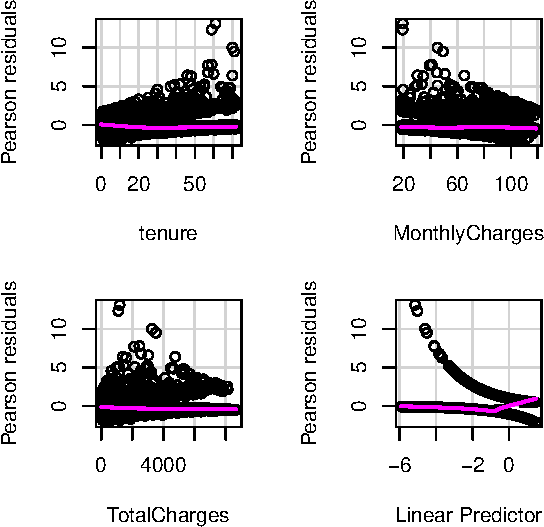
\includegraphics{Assigment2_files/figure-latex/unnamed-chunk-54-1.pdf}

\begin{verbatim}
##                Test stat Pr(>|Test stat|)   
## tenure           10.1732         0.001425 **
## MonthlyCharges    2.1562         0.141999   
## TotalCharges      0.0045         0.946457   
## ---
## Signif. codes:  0 '***' 0.001 '**' 0.01 '*' 0.05 '.' 0.1 ' ' 1
\end{verbatim}

The residuals need to be nearer to the 0 and they have homocedasticity.

\hypertarget{categorical-variables}{%
\subsubsection{Categorical Variables}\label{categorical-variables}}

Now, we shall add the categorical variables. The order of addition is
significant, therefore we start by adding the most correlated variables
with the target.

**Contract*

\begin{Shaded}
\begin{Highlighting}[]
\NormalTok{mod4 }\OtherTok{\textless{}{-}} \FunctionTok{glm}\NormalTok{(Churn }\SpecialCharTok{\textasciitilde{}}\NormalTok{ tenure }\SpecialCharTok{+}\NormalTok{ MonthlyCharges }\SpecialCharTok{+}\NormalTok{ Contract, }\AttributeTok{data=}\NormalTok{train, }\AttributeTok{family=}\NormalTok{binomial)}
\FunctionTok{AIC}\NormalTok{(mod4) }\CommentTok{\#4302.2 better}
\end{Highlighting}
\end{Shaded}

\begin{verbatim}
## [1] 4302.234
\end{verbatim}

\begin{Shaded}
\begin{Highlighting}[]
\FunctionTok{anova}\NormalTok{( mod3, mod4,  }\AttributeTok{test=}\StringTok{"Chisq"}\NormalTok{) }\CommentTok{\#significant}
\end{Highlighting}
\end{Shaded}

\begin{verbatim}
## Analysis of Deviance Table
## 
## Model 1: Churn ~ tenure + MonthlyCharges + TotalCharges
## Model 2: Churn ~ tenure + MonthlyCharges + Contract
##   Resid. Df Resid. Dev Df Deviance  Pr(>Chi)    
## 1      4926     4460.6                          
## 2      4925     4292.2  1   168.32 < 2.2e-16 ***
## ---
## Signif. codes:  0 '***' 0.001 '**' 0.01 '*' 0.05 '.' 0.1 ' ' 1
\end{verbatim}

\begin{Shaded}
\begin{Highlighting}[]
\FunctionTok{vif}\NormalTok{(mod4)}
\end{Highlighting}
\end{Shaded}

\begin{verbatim}
##                    GVIF Df GVIF^(1/(2*Df))
## tenure         1.707900  1        1.306867
## MonthlyCharges 1.300967  1        1.140599
## Contract       1.361428  2        1.080186
\end{verbatim}

We add the parameter because it improves the model.

\textbf{InternetService}

\begin{Shaded}
\begin{Highlighting}[]
\NormalTok{mod5 }\OtherTok{\textless{}{-}} \FunctionTok{glm}\NormalTok{(Churn }\SpecialCharTok{\textasciitilde{}}\NormalTok{ tenure }\SpecialCharTok{+}\NormalTok{ MonthlyCharges }\SpecialCharTok{+}\NormalTok{ Contract }\SpecialCharTok{+}\NormalTok{ InternetService, }\AttributeTok{data=}\NormalTok{train, }\AttributeTok{family=}\NormalTok{binomial)}
\FunctionTok{AIC}\NormalTok{(mod5) }\CommentTok{\#4254.1 better}
\end{Highlighting}
\end{Shaded}

\begin{verbatim}
## [1] 4254.114
\end{verbatim}

\begin{Shaded}
\begin{Highlighting}[]
\FunctionTok{anova}\NormalTok{( mod4, mod5,  }\AttributeTok{test=}\StringTok{"Chisq"}\NormalTok{) }\CommentTok{\#significant}
\end{Highlighting}
\end{Shaded}

\begin{verbatim}
## Analysis of Deviance Table
## 
## Model 1: Churn ~ tenure + MonthlyCharges + Contract
## Model 2: Churn ~ tenure + MonthlyCharges + Contract + InternetService
##   Resid. Df Resid. Dev Df Deviance  Pr(>Chi)    
## 1      4925     4292.2                          
## 2      4923     4240.1  2    52.12 4.811e-12 ***
## ---
## Signif. codes:  0 '***' 0.001 '**' 0.01 '*' 0.05 '.' 0.1 ' ' 1
\end{verbatim}

\begin{Shaded}
\begin{Highlighting}[]
\FunctionTok{vif}\NormalTok{(mod5)}
\end{Highlighting}
\end{Shaded}

\begin{verbatim}
##                     GVIF Df GVIF^(1/(2*Df))
## tenure          1.738643  1        1.318576
## MonthlyCharges  6.009378  1        2.451403
## Contract        1.450931  2        1.097518
## InternetService 5.338238  2        1.520021
\end{verbatim}

\textbf{StreamingMovies}

\begin{Shaded}
\begin{Highlighting}[]
\NormalTok{mod6 }\OtherTok{\textless{}{-}} \FunctionTok{glm}\NormalTok{(Churn }\SpecialCharTok{\textasciitilde{}}\NormalTok{ tenure }\SpecialCharTok{+}\NormalTok{ MonthlyCharges }\SpecialCharTok{+}\NormalTok{ Contract }\SpecialCharTok{+}\NormalTok{ InternetService }\SpecialCharTok{+} 
\NormalTok{              StreamingMovies, }\AttributeTok{data=}\NormalTok{train, }\AttributeTok{family=}\NormalTok{binomial)}
\FunctionTok{AIC}\NormalTok{(mod6) }\CommentTok{\#4238.6 better}
\end{Highlighting}
\end{Shaded}

\begin{verbatim}
## [1] 4238.552
\end{verbatim}

\begin{Shaded}
\begin{Highlighting}[]
\FunctionTok{anova}\NormalTok{( mod5, mod6,  }\AttributeTok{test=}\StringTok{"Chisq"}\NormalTok{) }\CommentTok{\#significant}
\end{Highlighting}
\end{Shaded}

\begin{verbatim}
## Analysis of Deviance Table
## 
## Model 1: Churn ~ tenure + MonthlyCharges + Contract + InternetService
## Model 2: Churn ~ tenure + MonthlyCharges + Contract + InternetService + 
##     StreamingMovies
##   Resid. Df Resid. Dev Df Deviance Pr(>Chi)    
## 1      4923     4240.1                         
## 2      4922     4222.6  1   17.563 2.78e-05 ***
## ---
## Signif. codes:  0 '***' 0.001 '**' 0.01 '*' 0.05 '.' 0.1 ' ' 1
\end{verbatim}

\begin{Shaded}
\begin{Highlighting}[]
\FunctionTok{vif}\NormalTok{(mod6)}
\end{Highlighting}
\end{Shaded}

\begin{verbatim}
##                     GVIF Df GVIF^(1/(2*Df))
## tenure          1.734387  1        1.316961
## MonthlyCharges  9.114445  1        3.019014
## Contract        1.447519  2        1.096872
## InternetService 6.680296  2        1.607677
## StreamingMovies 1.878425  1        1.370556
\end{verbatim}

The model has improved but the VIF is becoming higher.

\textbf{StreamingTV}

\begin{Shaded}
\begin{Highlighting}[]
\NormalTok{mod7 }\OtherTok{\textless{}{-}} \FunctionTok{glm}\NormalTok{(Churn }\SpecialCharTok{\textasciitilde{}}\NormalTok{ tenure }\SpecialCharTok{+}\NormalTok{ MonthlyCharges }\SpecialCharTok{+}\NormalTok{ Contract }\SpecialCharTok{+}\NormalTok{ InternetService }\SpecialCharTok{+} 
\NormalTok{              StreamingMovies }\SpecialCharTok{+}\NormalTok{ StreamingTV, }\AttributeTok{data=}\NormalTok{train, }\AttributeTok{family=}\NormalTok{binomial)}
\FunctionTok{AIC}\NormalTok{(mod7) }\CommentTok{\#4213.5 better}
\end{Highlighting}
\end{Shaded}

\begin{verbatim}
## [1] 4213.55
\end{verbatim}

\begin{Shaded}
\begin{Highlighting}[]
\FunctionTok{anova}\NormalTok{( mod6, mod7,  }\AttributeTok{test=}\StringTok{"Chisq"}\NormalTok{) }\CommentTok{\#significant}
\end{Highlighting}
\end{Shaded}

\begin{verbatim}
## Analysis of Deviance Table
## 
## Model 1: Churn ~ tenure + MonthlyCharges + Contract + InternetService + 
##     StreamingMovies
## Model 2: Churn ~ tenure + MonthlyCharges + Contract + InternetService + 
##     StreamingMovies + StreamingTV
##   Resid. Df Resid. Dev Df Deviance  Pr(>Chi)    
## 1      4922     4222.6                          
## 2      4921     4195.5  1   27.002 2.033e-07 ***
## ---
## Signif. codes:  0 '***' 0.001 '**' 0.01 '*' 0.05 '.' 0.1 ' ' 1
\end{verbatim}

\begin{Shaded}
\begin{Highlighting}[]
\FunctionTok{vif}\NormalTok{(mod7)}
\end{Highlighting}
\end{Shaded}

\begin{verbatim}
##                      GVIF Df GVIF^(1/(2*Df))
## tenure           1.732269  1        1.316157
## MonthlyCharges  12.166459  1        3.488045
## Contract         1.443988  2        1.096203
## InternetService  7.954251  2        1.679383
## StreamingMovies  1.860165  1        1.363878
## StreamingTV      1.906895  1        1.380904
\end{verbatim}

\emph{MonthlyCharges} has a high VIF. We'll may need to add
transformations or maybe discard this variable. For now, we will keep
the parameters that we have been adding.

\textbf{TechSupport}

\begin{Shaded}
\begin{Highlighting}[]
\NormalTok{mod8 }\OtherTok{\textless{}{-}} \FunctionTok{glm}\NormalTok{(Churn }\SpecialCharTok{\textasciitilde{}}\NormalTok{ tenure }\SpecialCharTok{+}\NormalTok{ MonthlyCharges }\SpecialCharTok{+}\NormalTok{ Contract }\SpecialCharTok{+}\NormalTok{ InternetService }\SpecialCharTok{+} 
\NormalTok{      StreamingMovies }\SpecialCharTok{+}\NormalTok{ StreamingTV }\SpecialCharTok{+}\NormalTok{ TechSupport, }\AttributeTok{data=}\NormalTok{train, }\AttributeTok{family=}\NormalTok{binomial)}
\CommentTok{\#summary(mod8) \#4208.3 better}
\FunctionTok{AIC}\NormalTok{(mod8)}
\end{Highlighting}
\end{Shaded}

\begin{verbatim}
## [1] 4208.273
\end{verbatim}

\begin{Shaded}
\begin{Highlighting}[]
\FunctionTok{anova}\NormalTok{( mod7, mod8,  }\AttributeTok{test=}\StringTok{"Chisq"}\NormalTok{) }\CommentTok{\#significant}
\end{Highlighting}
\end{Shaded}

\begin{verbatim}
## Analysis of Deviance Table
## 
## Model 1: Churn ~ tenure + MonthlyCharges + Contract + InternetService + 
##     StreamingMovies + StreamingTV
## Model 2: Churn ~ tenure + MonthlyCharges + Contract + InternetService + 
##     StreamingMovies + StreamingTV + TechSupport
##   Resid. Df Resid. Dev Df Deviance Pr(>Chi)   
## 1      4921     4195.5                        
## 2      4920     4188.3  1   7.2764 0.006987 **
## ---
## Signif. codes:  0 '***' 0.001 '**' 0.01 '*' 0.05 '.' 0.1 ' ' 1
\end{verbatim}

\begin{Shaded}
\begin{Highlighting}[]
\FunctionTok{vif}\NormalTok{(mod8)}
\end{Highlighting}
\end{Shaded}

\begin{verbatim}
##                      GVIF Df GVIF^(1/(2*Df))
## tenure           1.732344  1        1.316185
## MonthlyCharges  13.838376  1        3.719997
## Contract         1.475851  2        1.102201
## InternetService  9.342986  2        1.748322
## StreamingMovies  1.893830  1        1.376165
## StreamingTV      1.943568  1        1.394119
## TechSupport      1.294163  1        1.137613
\end{verbatim}

Including \emph{TechSupport} improves the model.

\textbf{DeviceProtection}

\begin{Shaded}
\begin{Highlighting}[]
\NormalTok{mod9 }\OtherTok{\textless{}{-}} \FunctionTok{glm}\NormalTok{(Churn }\SpecialCharTok{\textasciitilde{}}\NormalTok{ tenure }\SpecialCharTok{+}\NormalTok{ MonthlyCharges }\SpecialCharTok{+}\NormalTok{ Contract }\SpecialCharTok{+}\NormalTok{ InternetService }\SpecialCharTok{+} 
\NormalTok{            StreamingMovies }\SpecialCharTok{+}\NormalTok{ StreamingTV }\SpecialCharTok{+}\NormalTok{ TechSupport }\SpecialCharTok{+}\NormalTok{ DeviceProtection, }
            \AttributeTok{data=}\NormalTok{train, }\AttributeTok{family=}\NormalTok{binomial)}
\FunctionTok{summary}\NormalTok{(mod9) }\CommentTok{\#4209.3 worse}
\end{Highlighting}
\end{Shaded}

\begin{verbatim}
## 
## Call:
## glm(formula = Churn ~ tenure + MonthlyCharges + Contract + InternetService + 
##     StreamingMovies + StreamingTV + TechSupport + DeviceProtection, 
##     family = binomial, data = train)
## 
## Coefficients:
##                            Estimate Std. Error z value Pr(>|z|)    
## (Intercept)                 0.20725    0.24332   0.852 0.394345    
## tenure                     -0.03217    0.00250 -12.868  < 2e-16 ***
## MonthlyCharges             -0.01417    0.00558  -2.539 0.011129 *  
## ContractOne year           -0.84846    0.12453  -6.813 9.54e-12 ***
## ContractTwo year           -1.71130    0.21068  -8.123 4.55e-16 ***
## InternetServiceFiber optic  1.49636    0.20259   7.386 1.51e-13 ***
## InternetServiceNo          -1.33473    0.19328  -6.906 5.00e-12 ***
## StreamingMoviesYes          0.41040    0.10661   3.850 0.000118 ***
## StreamingTVYes              0.51843    0.10817   4.793 1.64e-06 ***
## TechSupportYes             -0.27817    0.10447  -2.663 0.007751 ** 
## DeviceProtectionYes         0.09141    0.09477   0.965 0.334789    
## ---
## Signif. codes:  0 '***' 0.001 '**' 0.01 '*' 0.05 '.' 0.1 ' ' 1
## 
## (Dispersion parameter for binomial family taken to be 1)
## 
##     Null deviance: 5694.2  on 4929  degrees of freedom
## Residual deviance: 4187.3  on 4919  degrees of freedom
## AIC: 4209.3
## 
## Number of Fisher Scoring iterations: 6
\end{verbatim}

\begin{Shaded}
\begin{Highlighting}[]
\FunctionTok{AIC}\NormalTok{(mod9)}
\end{Highlighting}
\end{Shaded}

\begin{verbatim}
## [1] 4209.343
\end{verbatim}

\begin{Shaded}
\begin{Highlighting}[]
\FunctionTok{anova}\NormalTok{( mod8, mod9,  }\AttributeTok{test=}\StringTok{"Chisq"}\NormalTok{) }\CommentTok{\#not significant}
\end{Highlighting}
\end{Shaded}

\begin{verbatim}
## Analysis of Deviance Table
## 
## Model 1: Churn ~ tenure + MonthlyCharges + Contract + InternetService + 
##     StreamingMovies + StreamingTV + TechSupport
## Model 2: Churn ~ tenure + MonthlyCharges + Contract + InternetService + 
##     StreamingMovies + StreamingTV + TechSupport + DeviceProtection
##   Resid. Df Resid. Dev Df Deviance Pr(>Chi)
## 1      4920     4188.3                     
## 2      4919     4187.3  1  0.93092   0.3346
\end{verbatim}

We don't add the variable to the model. It does not improve it.

\textbf{OnlineBackup}

\begin{Shaded}
\begin{Highlighting}[]
\NormalTok{mod10 }\OtherTok{\textless{}{-}} \FunctionTok{glm}\NormalTok{(Churn }\SpecialCharTok{\textasciitilde{}}\NormalTok{ tenure }\SpecialCharTok{+}\NormalTok{ MonthlyCharges }\SpecialCharTok{+}\NormalTok{ Contract }\SpecialCharTok{+}\NormalTok{ InternetService }\SpecialCharTok{+} 
\NormalTok{               StreamingMovies }\SpecialCharTok{+}\NormalTok{ StreamingTV }\SpecialCharTok{+}\NormalTok{ TechSupport }\SpecialCharTok{+}\NormalTok{ OnlineBackup, }
             \AttributeTok{data=}\NormalTok{train, }\AttributeTok{family=}\NormalTok{binomial)}
\FunctionTok{AIC}\NormalTok{(mod10) }\CommentTok{\#4209.6 worse}
\end{Highlighting}
\end{Shaded}

\begin{verbatim}
## [1] 4209.632
\end{verbatim}

\begin{Shaded}
\begin{Highlighting}[]
\FunctionTok{anova}\NormalTok{( mod8, mod10,  }\AttributeTok{test=}\StringTok{"Chisq"}\NormalTok{) }\CommentTok{\#not significant}
\end{Highlighting}
\end{Shaded}

\begin{verbatim}
## Analysis of Deviance Table
## 
## Model 1: Churn ~ tenure + MonthlyCharges + Contract + InternetService + 
##     StreamingMovies + StreamingTV + TechSupport
## Model 2: Churn ~ tenure + MonthlyCharges + Contract + InternetService + 
##     StreamingMovies + StreamingTV + TechSupport + OnlineBackup
##   Resid. Df Resid. Dev Df Deviance Pr(>Chi)
## 1      4920     4188.3                     
## 2      4919     4187.6  1  0.64158   0.4231
\end{verbatim}

We don't add the variable to the model. It does not improve it.

\textbf{OnlineSecurity}

\begin{Shaded}
\begin{Highlighting}[]
\NormalTok{mod11 }\OtherTok{\textless{}{-}} \FunctionTok{glm}\NormalTok{(Churn }\SpecialCharTok{\textasciitilde{}}\NormalTok{ tenure }\SpecialCharTok{+}\NormalTok{ MonthlyCharges }\SpecialCharTok{+}\NormalTok{ Contract }\SpecialCharTok{+}\NormalTok{ InternetService }\SpecialCharTok{+} 
\NormalTok{               StreamingMovies }\SpecialCharTok{+}\NormalTok{ StreamingTV }\SpecialCharTok{+}\NormalTok{ TechSupport }\SpecialCharTok{+}\NormalTok{ OnlineSecurity, }
             \AttributeTok{data=}\NormalTok{train, }\AttributeTok{family=}\NormalTok{binomial)}
\FunctionTok{AIC}\NormalTok{(mod11) }\CommentTok{\#4199 better}
\end{Highlighting}
\end{Shaded}

\begin{verbatim}
## [1] 4198.953
\end{verbatim}

\begin{Shaded}
\begin{Highlighting}[]
\FunctionTok{anova}\NormalTok{( mod8, mod11,  }\AttributeTok{test=}\StringTok{"Chisq"}\NormalTok{) }\CommentTok{\#significant}
\end{Highlighting}
\end{Shaded}

\begin{verbatim}
## Analysis of Deviance Table
## 
## Model 1: Churn ~ tenure + MonthlyCharges + Contract + InternetService + 
##     StreamingMovies + StreamingTV + TechSupport
## Model 2: Churn ~ tenure + MonthlyCharges + Contract + InternetService + 
##     StreamingMovies + StreamingTV + TechSupport + OnlineSecurity
##   Resid. Df Resid. Dev Df Deviance  Pr(>Chi)    
## 1      4920     4188.3                          
## 2      4919     4177.0  1   11.321 0.0007665 ***
## ---
## Signif. codes:  0 '***' 0.001 '**' 0.01 '*' 0.05 '.' 0.1 ' ' 1
\end{verbatim}

\begin{Shaded}
\begin{Highlighting}[]
\FunctionTok{vif}\NormalTok{(mod11)}
\end{Highlighting}
\end{Shaded}

\begin{verbatim}
##                      GVIF Df GVIF^(1/(2*Df))
## tenure           1.744624  1        1.320842
## MonthlyCharges  15.487373  1        3.935400
## Contract         1.492903  2        1.105371
## InternetService 10.866851  2        1.815624
## StreamingMovies  1.971177  1        1.403986
## StreamingTV      2.028530  1        1.424265
## TechSupport      1.296059  1        1.138446
## OnlineSecurity   1.242751  1        1.114787
\end{verbatim}

We keep the variable. We still have multicollinearity, but we'll deal
with it later.

\textbf{PaperlessBilling}

\begin{Shaded}
\begin{Highlighting}[]
\NormalTok{mod12 }\OtherTok{\textless{}{-}} \FunctionTok{glm}\NormalTok{(Churn }\SpecialCharTok{\textasciitilde{}}\NormalTok{ tenure }\SpecialCharTok{+}\NormalTok{ MonthlyCharges }\SpecialCharTok{+}\NormalTok{ Contract }\SpecialCharTok{+}\NormalTok{ InternetService }\SpecialCharTok{+} 
\NormalTok{               StreamingMovies }\SpecialCharTok{+}\NormalTok{ StreamingTV }\SpecialCharTok{+}\NormalTok{ TechSupport }\SpecialCharTok{+}\NormalTok{ OnlineSecurity }\SpecialCharTok{+}
\NormalTok{               PaperlessBilling, }\AttributeTok{data=}\NormalTok{train, }\AttributeTok{family=}\NormalTok{binomial)}
\FunctionTok{summary}\NormalTok{(mod12) }\CommentTok{\#4184.5 better}
\end{Highlighting}
\end{Shaded}

\begin{verbatim}
## 
## Call:
## glm(formula = Churn ~ tenure + MonthlyCharges + Contract + InternetService + 
##     StreamingMovies + StreamingTV + TechSupport + OnlineSecurity + 
##     PaperlessBilling, family = binomial, data = train)
## 
## Coefficients:
##                             Estimate Std. Error z value Pr(>|z|)    
## (Intercept)                -0.206715   0.251517  -0.822 0.411150    
## tenure                     -0.031980   0.002512 -12.730  < 2e-16 ***
## MonthlyCharges             -0.006893   0.005737  -1.202 0.229554    
## ContractOne year           -0.774511   0.125366  -6.178 6.49e-10 ***
## ContractTwo year           -1.575801   0.211901  -7.436 1.03e-13 ***
## InternetServiceFiber optic  1.162390   0.211629   5.493 3.96e-08 ***
## InternetServiceNo          -1.216241   0.195326  -6.227 4.76e-10 ***
## StreamingMoviesYes          0.328093   0.109142   3.006 0.002646 ** 
## StreamingTVYes              0.412453   0.111023   3.715 0.000203 ***
## TechSupportYes             -0.293252   0.105072  -2.791 0.005255 ** 
## OnlineSecurityYes          -0.325252   0.105781  -3.075 0.002107 ** 
## PaperlessBillingYes         0.354796   0.087670   4.047 5.19e-05 ***
## ---
## Signif. codes:  0 '***' 0.001 '**' 0.01 '*' 0.05 '.' 0.1 ' ' 1
## 
## (Dispersion parameter for binomial family taken to be 1)
## 
##     Null deviance: 5694.2  on 4929  degrees of freedom
## Residual deviance: 4160.5  on 4918  degrees of freedom
## AIC: 4184.5
## 
## Number of Fisher Scoring iterations: 6
\end{verbatim}

\begin{Shaded}
\begin{Highlighting}[]
\FunctionTok{AIC}\NormalTok{(mod12)}
\end{Highlighting}
\end{Shaded}

\begin{verbatim}
## [1] 4184.475
\end{verbatim}

\begin{Shaded}
\begin{Highlighting}[]
\FunctionTok{anova}\NormalTok{( mod11, mod12,  }\AttributeTok{test=}\StringTok{"Chisq"}\NormalTok{) }\CommentTok{\#significant}
\end{Highlighting}
\end{Shaded}

\begin{verbatim}
## Analysis of Deviance Table
## 
## Model 1: Churn ~ tenure + MonthlyCharges + Contract + InternetService + 
##     StreamingMovies + StreamingTV + TechSupport + OnlineSecurity
## Model 2: Churn ~ tenure + MonthlyCharges + Contract + InternetService + 
##     StreamingMovies + StreamingTV + TechSupport + OnlineSecurity + 
##     PaperlessBilling
##   Resid. Df Resid. Dev Df Deviance  Pr(>Chi)    
## 1      4919     4177.0                          
## 2      4918     4160.5  1   16.478 4.923e-05 ***
## ---
## Signif. codes:  0 '***' 0.001 '**' 0.01 '*' 0.05 '.' 0.1 ' ' 1
\end{verbatim}

\begin{Shaded}
\begin{Highlighting}[]
\FunctionTok{vif}\NormalTok{(mod12)}
\end{Highlighting}
\end{Shaded}

\begin{verbatim}
##                       GVIF Df GVIF^(1/(2*Df))
## tenure            1.760119  1        1.326695
## MonthlyCharges   15.519259  1        3.939449
## Contract          1.507661  2        1.108092
## InternetService  10.973792  2        1.820075
## StreamingMovies   1.970408  1        1.403712
## StreamingTV       2.035605  1        1.426746
## TechSupport       1.298079  1        1.139333
## OnlineSecurity    1.247294  1        1.116823
## PaperlessBilling  1.111928  1        1.054480
\end{verbatim}

We keep the variable because it improves the model.

\textbf{Dependents}

\begin{Shaded}
\begin{Highlighting}[]
\NormalTok{mod13 }\OtherTok{\textless{}{-}} \FunctionTok{glm}\NormalTok{(Churn }\SpecialCharTok{\textasciitilde{}}\NormalTok{ tenure }\SpecialCharTok{+}\NormalTok{ MonthlyCharges }\SpecialCharTok{+}\NormalTok{ Contract }\SpecialCharTok{+}\NormalTok{ InternetService }\SpecialCharTok{+} 
\NormalTok{               StreamingMovies }\SpecialCharTok{+}\NormalTok{ StreamingTV }\SpecialCharTok{+}\NormalTok{ TechSupport }\SpecialCharTok{+}\NormalTok{ OnlineSecurity }\SpecialCharTok{+} 
\NormalTok{               PaperlessBilling }\SpecialCharTok{+}\NormalTok{ Dependents, }\AttributeTok{data=}\NormalTok{train, }\AttributeTok{family=}\NormalTok{binomial)}
\FunctionTok{summary}\NormalTok{(mod13) }\CommentTok{\#4177.2 better}
\end{Highlighting}
\end{Shaded}

\begin{verbatim}
## 
## Call:
## glm(formula = Churn ~ tenure + MonthlyCharges + Contract + InternetService + 
##     StreamingMovies + StreamingTV + TechSupport + OnlineSecurity + 
##     PaperlessBilling + Dependents, family = binomial, data = train)
## 
## Coefficients:
##                             Estimate Std. Error z value Pr(>|z|)    
## (Intercept)                -0.160331   0.252462  -0.635  0.52538    
## tenure                     -0.031654   0.002520 -12.559  < 2e-16 ***
## MonthlyCharges             -0.006595   0.005749  -1.147  0.25137    
## ContractOne year           -0.746604   0.125870  -5.932 3.00e-09 ***
## ContractTwo year           -1.536143   0.212595  -7.226 4.99e-13 ***
## InternetServiceFiber optic  1.133942   0.212173   5.344 9.07e-08 ***
## InternetServiceNo          -1.193933   0.195766  -6.099 1.07e-09 ***
## StreamingMoviesYes          0.317729   0.109348   2.906  0.00366 ** 
## StreamingTVYes              0.412210   0.111213   3.706  0.00021 ***
## TechSupportYes             -0.287327   0.105193  -2.731  0.00631 ** 
## OnlineSecurityYes          -0.317077   0.105920  -2.994  0.00276 ** 
## PaperlessBillingYes         0.351625   0.087803   4.005 6.21e-05 ***
## DependentsYes              -0.291003   0.096298  -3.022  0.00251 ** 
## ---
## Signif. codes:  0 '***' 0.001 '**' 0.01 '*' 0.05 '.' 0.1 ' ' 1
## 
## (Dispersion parameter for binomial family taken to be 1)
## 
##     Null deviance: 5694.2  on 4929  degrees of freedom
## Residual deviance: 4151.2  on 4917  degrees of freedom
## AIC: 4177.2
## 
## Number of Fisher Scoring iterations: 6
\end{verbatim}

\begin{Shaded}
\begin{Highlighting}[]
\FunctionTok{AIC}\NormalTok{(mod13)}
\end{Highlighting}
\end{Shaded}

\begin{verbatim}
## [1] 4177.206
\end{verbatim}

\begin{Shaded}
\begin{Highlighting}[]
\FunctionTok{anova}\NormalTok{( mod12, mod13,  }\AttributeTok{test=}\StringTok{"Chisq"}\NormalTok{) }\CommentTok{\#significant}
\end{Highlighting}
\end{Shaded}

\begin{verbatim}
## Analysis of Deviance Table
## 
## Model 1: Churn ~ tenure + MonthlyCharges + Contract + InternetService + 
##     StreamingMovies + StreamingTV + TechSupport + OnlineSecurity + 
##     PaperlessBilling
## Model 2: Churn ~ tenure + MonthlyCharges + Contract + InternetService + 
##     StreamingMovies + StreamingTV + TechSupport + OnlineSecurity + 
##     PaperlessBilling + Dependents
##   Resid. Df Resid. Dev Df Deviance Pr(>Chi)   
## 1      4918     4160.5                        
## 2      4917     4151.2  1   9.2692  0.00233 **
## ---
## Signif. codes:  0 '***' 0.001 '**' 0.01 '*' 0.05 '.' 0.1 ' ' 1
\end{verbatim}

\begin{Shaded}
\begin{Highlighting}[]
\FunctionTok{vif}\NormalTok{(mod13)}
\end{Highlighting}
\end{Shaded}

\begin{verbatim}
##                       GVIF Df GVIF^(1/(2*Df))
## tenure            1.773404  1        1.331692
## MonthlyCharges   15.562560  1        3.944941
## Contract          1.522708  2        1.110847
## InternetService  10.992492  2        1.820849
## StreamingMovies   1.973305  1        1.404744
## StreamingTV       2.037770  1        1.427505
## TechSupport       1.299374  1        1.139901
## OnlineSecurity    1.247956  1        1.117120
## PaperlessBilling  1.112626  1        1.054811
## Dependents        1.027601  1        1.013706
\end{verbatim}

We keep the variable because it improves the model.

\textbf{MultipleLines}

\begin{Shaded}
\begin{Highlighting}[]
\NormalTok{mod14 }\OtherTok{\textless{}{-}} \FunctionTok{glm}\NormalTok{(Churn }\SpecialCharTok{\textasciitilde{}}\NormalTok{ tenure }\SpecialCharTok{+}\NormalTok{ MonthlyCharges }\SpecialCharTok{+}\NormalTok{ Contract }\SpecialCharTok{+}\NormalTok{ InternetService }\SpecialCharTok{+} 
\NormalTok{               StreamingMovies }\SpecialCharTok{+}\NormalTok{ StreamingTV }\SpecialCharTok{+}\NormalTok{ TechSupport }\SpecialCharTok{+}\NormalTok{ OnlineSecurity }\SpecialCharTok{+} 
\NormalTok{               PaperlessBilling }\SpecialCharTok{+}\NormalTok{ Dependents }\SpecialCharTok{+}\NormalTok{ MultipleLines,}
             \AttributeTok{data=}\NormalTok{train, }\AttributeTok{family=}\NormalTok{binomial)}
\FunctionTok{AIC}\NormalTok{(mod14) }\CommentTok{\#4162.2 better}
\end{Highlighting}
\end{Shaded}

\begin{verbatim}
## [1] 4162.18
\end{verbatim}

\begin{Shaded}
\begin{Highlighting}[]
\FunctionTok{anova}\NormalTok{( mod13, mod14,  }\AttributeTok{test=}\StringTok{"Chisq"}\NormalTok{) }\CommentTok{\#significant}
\end{Highlighting}
\end{Shaded}

\begin{verbatim}
## Analysis of Deviance Table
## 
## Model 1: Churn ~ tenure + MonthlyCharges + Contract + InternetService + 
##     StreamingMovies + StreamingTV + TechSupport + OnlineSecurity + 
##     PaperlessBilling + Dependents
## Model 2: Churn ~ tenure + MonthlyCharges + Contract + InternetService + 
##     StreamingMovies + StreamingTV + TechSupport + OnlineSecurity + 
##     PaperlessBilling + Dependents + MultipleLines
##   Resid. Df Resid. Dev Df Deviance  Pr(>Chi)    
## 1      4917     4151.2                          
## 2      4916     4134.2  1   17.026 3.688e-05 ***
## ---
## Signif. codes:  0 '***' 0.001 '**' 0.01 '*' 0.05 '.' 0.1 ' ' 1
\end{verbatim}

\begin{Shaded}
\begin{Highlighting}[]
\FunctionTok{vif}\NormalTok{(mod14)}
\end{Highlighting}
\end{Shaded}

\begin{verbatim}
##                       GVIF Df GVIF^(1/(2*Df))
## tenure            1.860860  1        1.364133
## MonthlyCharges   19.785122  1        4.448047
## Contract          1.529039  2        1.112000
## InternetService  12.562934  2        1.882664
## StreamingMovies   2.104685  1        1.450753
## StreamingTV       2.150829  1        1.466570
## TechSupport       1.346109  1        1.160219
## OnlineSecurity    1.283323  1        1.132838
## PaperlessBilling  1.113149  1        1.055059
## Dependents        1.028391  1        1.014096
## MultipleLines     1.749163  1        1.322559
\end{verbatim}

We keep the variable because it improves the model.

\textbf{SeniorCitizen}

\begin{Shaded}
\begin{Highlighting}[]
\NormalTok{mod15 }\OtherTok{\textless{}{-}} \FunctionTok{glm}\NormalTok{(Churn }\SpecialCharTok{\textasciitilde{}}\NormalTok{ tenure }\SpecialCharTok{+}\NormalTok{ MonthlyCharges }\SpecialCharTok{+}\NormalTok{ Contract }\SpecialCharTok{+}\NormalTok{ InternetService }\SpecialCharTok{+}
\NormalTok{               StreamingMovies }\SpecialCharTok{+}\NormalTok{ StreamingTV }\SpecialCharTok{+}\NormalTok{ TechSupport }\SpecialCharTok{+}\NormalTok{ OnlineSecurity }\SpecialCharTok{+}
\NormalTok{               PaperlessBilling }\SpecialCharTok{+}\NormalTok{ Dependents }\SpecialCharTok{+}\NormalTok{ MultipleLines }\SpecialCharTok{+}\NormalTok{ SeniorCitizen,}
             \AttributeTok{data=}\NormalTok{train, }\AttributeTok{family=}\NormalTok{binomial)}
\FunctionTok{AIC}\NormalTok{(mod15) }\CommentTok{\#4155.7 better}
\end{Highlighting}
\end{Shaded}

\begin{verbatim}
## [1] 4155.702
\end{verbatim}

\begin{Shaded}
\begin{Highlighting}[]
\FunctionTok{anova}\NormalTok{( mod14, mod15,  }\AttributeTok{test=}\StringTok{"Chisq"}\NormalTok{) }\CommentTok{\#significant}
\end{Highlighting}
\end{Shaded}

\begin{verbatim}
## Analysis of Deviance Table
## 
## Model 1: Churn ~ tenure + MonthlyCharges + Contract + InternetService + 
##     StreamingMovies + StreamingTV + TechSupport + OnlineSecurity + 
##     PaperlessBilling + Dependents + MultipleLines
## Model 2: Churn ~ tenure + MonthlyCharges + Contract + InternetService + 
##     StreamingMovies + StreamingTV + TechSupport + OnlineSecurity + 
##     PaperlessBilling + Dependents + MultipleLines + SeniorCitizen
##   Resid. Df Resid. Dev Df Deviance Pr(>Chi)   
## 1      4916     4134.2                        
## 2      4915     4125.7  1   8.4782 0.003594 **
## ---
## Signif. codes:  0 '***' 0.001 '**' 0.01 '*' 0.05 '.' 0.1 ' ' 1
\end{verbatim}

\begin{Shaded}
\begin{Highlighting}[]
\FunctionTok{vif}\NormalTok{(mod15)}
\end{Highlighting}
\end{Shaded}

\begin{verbatim}
##                       GVIF Df GVIF^(1/(2*Df))
## tenure            1.889241  1        1.374497
## MonthlyCharges   19.790331  1        4.448632
## Contract          1.536772  2        1.113403
## InternetService  12.635139  2        1.885363
## StreamingMovies   2.104216  1        1.450592
## StreamingTV       2.148543  1        1.465791
## TechSupport       1.353673  1        1.163474
## OnlineSecurity    1.286526  1        1.134251
## PaperlessBilling  1.114284  1        1.055597
## Dependents        1.056349  1        1.027789
## MultipleLines     1.752169  1        1.323695
## SeniorCitizen     1.113813  1        1.055374
\end{verbatim}

We keep the variable because it improves the model.

\textbf{Partner}

\begin{Shaded}
\begin{Highlighting}[]
\NormalTok{mod16 }\OtherTok{\textless{}{-}} \FunctionTok{glm}\NormalTok{(Churn }\SpecialCharTok{\textasciitilde{}}\NormalTok{ tenure }\SpecialCharTok{+}\NormalTok{ MonthlyCharges }\SpecialCharTok{+}\NormalTok{ Contract }\SpecialCharTok{+}\NormalTok{ InternetService }\SpecialCharTok{+} 
\NormalTok{               StreamingMovies }\SpecialCharTok{+}\NormalTok{ StreamingTV }\SpecialCharTok{+}\NormalTok{ TechSupport }\SpecialCharTok{+}\NormalTok{ OnlineSecurity }\SpecialCharTok{+} 
\NormalTok{               PaperlessBilling }\SpecialCharTok{+}\NormalTok{ Dependents }\SpecialCharTok{+}\NormalTok{ MultipleLines }\SpecialCharTok{+}\NormalTok{ SeniorCitizen }\SpecialCharTok{+} 
\NormalTok{               Partner, }\AttributeTok{data=}\NormalTok{train, }\AttributeTok{family=}\NormalTok{binomial)}
\FunctionTok{AIC}\NormalTok{(mod16) }\CommentTok{\#4157.7 worse}
\end{Highlighting}
\end{Shaded}

\begin{verbatim}
## [1] 4157.677
\end{verbatim}

\begin{Shaded}
\begin{Highlighting}[]
\FunctionTok{anova}\NormalTok{( mod15, mod16,  }\AttributeTok{test=}\StringTok{"Chisq"}\NormalTok{) }\CommentTok{\#not significant}
\end{Highlighting}
\end{Shaded}

\begin{verbatim}
## Analysis of Deviance Table
## 
## Model 1: Churn ~ tenure + MonthlyCharges + Contract + InternetService + 
##     StreamingMovies + StreamingTV + TechSupport + OnlineSecurity + 
##     PaperlessBilling + Dependents + MultipleLines + SeniorCitizen
## Model 2: Churn ~ tenure + MonthlyCharges + Contract + InternetService + 
##     StreamingMovies + StreamingTV + TechSupport + OnlineSecurity + 
##     PaperlessBilling + Dependents + MultipleLines + SeniorCitizen + 
##     Partner
##   Resid. Df Resid. Dev Df Deviance Pr(>Chi)
## 1      4915     4125.7                     
## 2      4914     4125.7  1 0.024971   0.8744
\end{verbatim}

We don't keep the variable because it does not improve the model.

\textbf{PaymentMethod}

\begin{Shaded}
\begin{Highlighting}[]
\NormalTok{mod17 }\OtherTok{\textless{}{-}} \FunctionTok{glm}\NormalTok{(Churn }\SpecialCharTok{\textasciitilde{}}\NormalTok{ tenure }\SpecialCharTok{+}\NormalTok{ MonthlyCharges }\SpecialCharTok{+}\NormalTok{ Contract }\SpecialCharTok{+}\NormalTok{ InternetService }\SpecialCharTok{+} 
\NormalTok{               StreamingMovies }\SpecialCharTok{+}\NormalTok{ StreamingTV }\SpecialCharTok{+}\NormalTok{ TechSupport }\SpecialCharTok{+}\NormalTok{ OnlineSecurity }\SpecialCharTok{+} 
\NormalTok{               PaperlessBilling }\SpecialCharTok{+}\NormalTok{ Dependents }\SpecialCharTok{+}\NormalTok{ MultipleLines }\SpecialCharTok{+}\NormalTok{ SeniorCitizen }\SpecialCharTok{+} 
\NormalTok{               PaymentMethod, }\AttributeTok{data=}\NormalTok{train, }\AttributeTok{family=}\NormalTok{binomial) }
\FunctionTok{AIC}\NormalTok{(mod17) }\CommentTok{\#4139.4 better}
\end{Highlighting}
\end{Shaded}

\begin{verbatim}
## [1] 4139.434
\end{verbatim}

\begin{Shaded}
\begin{Highlighting}[]
\FunctionTok{anova}\NormalTok{( mod15, mod17,  }\AttributeTok{test=}\StringTok{"Chisq"}\NormalTok{) }\CommentTok{\#significant}
\end{Highlighting}
\end{Shaded}

\begin{verbatim}
## Analysis of Deviance Table
## 
## Model 1: Churn ~ tenure + MonthlyCharges + Contract + InternetService + 
##     StreamingMovies + StreamingTV + TechSupport + OnlineSecurity + 
##     PaperlessBilling + Dependents + MultipleLines + SeniorCitizen
## Model 2: Churn ~ tenure + MonthlyCharges + Contract + InternetService + 
##     StreamingMovies + StreamingTV + TechSupport + OnlineSecurity + 
##     PaperlessBilling + Dependents + MultipleLines + SeniorCitizen + 
##     PaymentMethod
##   Resid. Df Resid. Dev Df Deviance  Pr(>Chi)    
## 1      4915     4125.7                          
## 2      4912     4103.4  3   22.269 5.735e-05 ***
## ---
## Signif. codes:  0 '***' 0.001 '**' 0.01 '*' 0.05 '.' 0.1 ' ' 1
\end{verbatim}

\begin{Shaded}
\begin{Highlighting}[]
\FunctionTok{vif}\NormalTok{(mod17)}
\end{Highlighting}
\end{Shaded}

\begin{verbatim}
##                       GVIF Df GVIF^(1/(2*Df))
## tenure            1.963626  1        1.401295
## MonthlyCharges   19.895259  1        4.460410
## Contract          1.543913  2        1.114694
## InternetService  13.046889  2        1.900539
## StreamingMovies   2.110866  1        1.452882
## StreamingTV       2.164001  1        1.471054
## TechSupport       1.357356  1        1.165056
## OnlineSecurity    1.291867  1        1.136603
## PaperlessBilling  1.120742  1        1.058651
## Dependents        1.057502  1        1.028349
## MultipleLines     1.753352  1        1.324142
## SeniorCitizen     1.116591  1        1.056689
## PaymentMethod     1.332467  3        1.049001
\end{verbatim}

We keep the variable because it improves the model.

\textbf{PhoneService}

\begin{Shaded}
\begin{Highlighting}[]
\NormalTok{mod18 }\OtherTok{\textless{}{-}} \FunctionTok{glm}\NormalTok{(Churn }\SpecialCharTok{\textasciitilde{}}\NormalTok{ tenure }\SpecialCharTok{+}\NormalTok{ MonthlyCharges }\SpecialCharTok{+}\NormalTok{ Contract }\SpecialCharTok{+}\NormalTok{ InternetService }\SpecialCharTok{+} 
\NormalTok{               StreamingMovies }\SpecialCharTok{+}\NormalTok{ StreamingTV }\SpecialCharTok{+}\NormalTok{ TechSupport }\SpecialCharTok{+}\NormalTok{ OnlineSecurity }\SpecialCharTok{+} 
\NormalTok{               PaperlessBilling }\SpecialCharTok{+}\NormalTok{ Dependents }\SpecialCharTok{+}\NormalTok{ MultipleLines }\SpecialCharTok{+}\NormalTok{ SeniorCitizen }\SpecialCharTok{+} 
\NormalTok{               PaymentMethod }\SpecialCharTok{+}\NormalTok{ PhoneService, }\AttributeTok{data=}\NormalTok{train, }\AttributeTok{family=}\NormalTok{binomial)}
\FunctionTok{AIC}\NormalTok{(mod18)}\CommentTok{\#4139.4 it does not change anything}
\end{Highlighting}
\end{Shaded}

\begin{verbatim}
## [1] 4139.379
\end{verbatim}

\begin{Shaded}
\begin{Highlighting}[]
\FunctionTok{anova}\NormalTok{( mod17, mod18,  }\AttributeTok{test=}\StringTok{"Chisq"}\NormalTok{) }\CommentTok{\#not significant}
\end{Highlighting}
\end{Shaded}

\begin{verbatim}
## Analysis of Deviance Table
## 
## Model 1: Churn ~ tenure + MonthlyCharges + Contract + InternetService + 
##     StreamingMovies + StreamingTV + TechSupport + OnlineSecurity + 
##     PaperlessBilling + Dependents + MultipleLines + SeniorCitizen + 
##     PaymentMethod
## Model 2: Churn ~ tenure + MonthlyCharges + Contract + InternetService + 
##     StreamingMovies + StreamingTV + TechSupport + OnlineSecurity + 
##     PaperlessBilling + Dependents + MultipleLines + SeniorCitizen + 
##     PaymentMethod + PhoneService
##   Resid. Df Resid. Dev Df Deviance Pr(>Chi)
## 1      4912     4103.4                     
## 2      4911     4101.4  1    2.055   0.1517
\end{verbatim}

We don't include the parameter because it does not improve the model.

\hypertarget{inlfuential-data-1}{%
\subsubsection{Inlfuential data}\label{inlfuential-data-1}}

We check the influential data after including all categorical variables
.

\begin{Shaded}
\begin{Highlighting}[]
\NormalTok{infl\_2 }\OtherTok{\textless{}{-}} \FunctionTok{influence.measures}\NormalTok{(mod17)}

\FunctionTok{sum}\NormalTok{(}\FunctionTok{residuals}\NormalTok{(mod17,}\StringTok{\textquotesingle{}deviance\textquotesingle{}}\NormalTok{)}\SpecialCharTok{\^{}}\DecValTok{2}\NormalTok{)}
\end{Highlighting}
\end{Shaded}

\begin{verbatim}
## [1] 4103.434
\end{verbatim}

\begin{Shaded}
\begin{Highlighting}[]
\FunctionTok{sum}\NormalTok{(}\FunctionTok{residuals}\NormalTok{(mod17,}\StringTok{\textquotesingle{}pearson\textquotesingle{}}\NormalTok{)}\SpecialCharTok{\^{}}\DecValTok{2}\NormalTok{)}
\end{Highlighting}
\end{Shaded}

\begin{verbatim}
## [1] 4919.679
\end{verbatim}

\begin{Shaded}
\begin{Highlighting}[]
\NormalTok{influential\_indices\_2 }\OtherTok{\textless{}{-}} \FunctionTok{which}\NormalTok{(infl\_2}\SpecialCharTok{$}\NormalTok{is.inf }\SpecialCharTok{==} \ConstantTok{TRUE}\NormalTok{)}
\FunctionTok{length}\NormalTok{(influential\_indices\_2)}
\end{Highlighting}
\end{Shaded}

\begin{verbatim}
## [1] 98
\end{verbatim}

\begin{Shaded}
\begin{Highlighting}[]
\FunctionTok{length}\NormalTok{(train}\SpecialCharTok{$}\NormalTok{customerID)}
\end{Highlighting}
\end{Shaded}

\begin{verbatim}
## [1] 4930
\end{verbatim}

The influential data has reduced until 98 tuples.

\hypertarget{interactions}{%
\subsubsection{Interactions}\label{interactions}}

We need to search for interactions. Possible interactions:

\hypertarget{dependents-and-multiple-lines}{%
\paragraph{Dependents and Multiple
Lines}\label{dependents-and-multiple-lines}}

\begin{Shaded}
\begin{Highlighting}[]
\NormalTok{mod19 }\OtherTok{\textless{}{-}} \FunctionTok{glm}\NormalTok{(Churn }\SpecialCharTok{\textasciitilde{}}\NormalTok{ tenure }\SpecialCharTok{+}\NormalTok{ MonthlyCharges }\SpecialCharTok{+}\NormalTok{ Contract }\SpecialCharTok{+}\NormalTok{ InternetService }\SpecialCharTok{+} 
\NormalTok{               StreamingMovies }\SpecialCharTok{+}\NormalTok{ StreamingTV }\SpecialCharTok{+}\NormalTok{ TechSupport }\SpecialCharTok{+}\NormalTok{ OnlineSecurity }\SpecialCharTok{+}
\NormalTok{               PaperlessBilling }\SpecialCharTok{+}\NormalTok{ Dependents }\SpecialCharTok{*}\NormalTok{ MultipleLines }\SpecialCharTok{+}\NormalTok{ SeniorCitizen }\SpecialCharTok{+} 
\NormalTok{               PaymentMethod, }\AttributeTok{data=}\NormalTok{train, }\AttributeTok{family=}\NormalTok{binomial)}
 \CommentTok{\#4140.4 worse}
\FunctionTok{AIC}\NormalTok{(mod19)}
\end{Highlighting}
\end{Shaded}

\begin{verbatim}
## [1] 4140.355
\end{verbatim}

\begin{Shaded}
\begin{Highlighting}[]
\FunctionTok{anova}\NormalTok{( mod17, mod19,  }\AttributeTok{test=}\StringTok{"Chisq"}\NormalTok{) }\CommentTok{\#not significant}
\end{Highlighting}
\end{Shaded}

\begin{verbatim}
## Analysis of Deviance Table
## 
## Model 1: Churn ~ tenure + MonthlyCharges + Contract + InternetService + 
##     StreamingMovies + StreamingTV + TechSupport + OnlineSecurity + 
##     PaperlessBilling + Dependents + MultipleLines + SeniorCitizen + 
##     PaymentMethod
## Model 2: Churn ~ tenure + MonthlyCharges + Contract + InternetService + 
##     StreamingMovies + StreamingTV + TechSupport + OnlineSecurity + 
##     PaperlessBilling + Dependents * MultipleLines + SeniorCitizen + 
##     PaymentMethod
##   Resid. Df Resid. Dev Df Deviance Pr(>Chi)
## 1      4912     4103.4                     
## 2      4911     4102.4  1   1.0787    0.299
\end{verbatim}

We don't include the interaction since it is not significative

\textbf{MonthlyCharges and InternetService}

\begin{Shaded}
\begin{Highlighting}[]
\NormalTok{mod20 }\OtherTok{\textless{}{-}} \FunctionTok{glm}\NormalTok{(Churn }\SpecialCharTok{\textasciitilde{}}\NormalTok{ tenure }\SpecialCharTok{+}\NormalTok{ InternetService }\SpecialCharTok{*}\NormalTok{ MonthlyCharges }\SpecialCharTok{+}\NormalTok{ Contract }\SpecialCharTok{+} 
\NormalTok{               StreamingMovies }\SpecialCharTok{+}\NormalTok{ StreamingTV }\SpecialCharTok{+}\NormalTok{ TechSupport }\SpecialCharTok{+}\NormalTok{ OnlineSecurity }\SpecialCharTok{+} 
\NormalTok{               PaperlessBilling }\SpecialCharTok{+}\NormalTok{ Dependents }\SpecialCharTok{+}\NormalTok{ MultipleLines }\SpecialCharTok{+}\NormalTok{ SeniorCitizen }\SpecialCharTok{+} 
\NormalTok{               PaymentMethod, }\AttributeTok{data=}\NormalTok{train, }\AttributeTok{family=}\NormalTok{binomial)}
\FunctionTok{AIC}\NormalTok{(mod20) }\CommentTok{\#4133.7 better}
\end{Highlighting}
\end{Shaded}

\begin{verbatim}
## [1] 4133.664
\end{verbatim}

\begin{Shaded}
\begin{Highlighting}[]
\FunctionTok{anova}\NormalTok{( mod17, mod20,  }\AttributeTok{test=}\StringTok{"Chisq"}\NormalTok{) }\CommentTok{\#significant}
\end{Highlighting}
\end{Shaded}

\begin{verbatim}
## Analysis of Deviance Table
## 
## Model 1: Churn ~ tenure + MonthlyCharges + Contract + InternetService + 
##     StreamingMovies + StreamingTV + TechSupport + OnlineSecurity + 
##     PaperlessBilling + Dependents + MultipleLines + SeniorCitizen + 
##     PaymentMethod
## Model 2: Churn ~ tenure + InternetService * MonthlyCharges + Contract + 
##     StreamingMovies + StreamingTV + TechSupport + OnlineSecurity + 
##     PaperlessBilling + Dependents + MultipleLines + SeniorCitizen + 
##     PaymentMethod
##   Resid. Df Resid. Dev Df Deviance Pr(>Chi)   
## 1      4912     4103.4                        
## 2      4910     4093.7  2   9.7694 0.007561 **
## ---
## Signif. codes:  0 '***' 0.001 '**' 0.01 '*' 0.05 '.' 0.1 ' ' 1
\end{verbatim}

\begin{Shaded}
\begin{Highlighting}[]
\FunctionTok{vif}\NormalTok{(mod20)}
\end{Highlighting}
\end{Shaded}

\begin{verbatim}
## there are higher-order terms (interactions) in this model
## consider setting type = 'predictor'; see ?vif
\end{verbatim}

\begin{verbatim}
##                                        GVIF Df GVIF^(1/(2*Df))
## tenure                             2.079881  1        1.442179
## InternetService                 9738.807709  2        9.934052
## MonthlyCharges                    21.386127  1        4.624514
## Contract                           1.550405  2        1.115864
## StreamingMovies                    2.374759  1        1.541025
## StreamingTV                        2.416906  1        1.554640
## TechSupport                        1.374225  1        1.172273
## OnlineSecurity                     1.300790  1        1.140522
## PaperlessBilling                   1.124965  1        1.060644
## Dependents                         1.056690  1        1.027954
## MultipleLines                      1.897486  1        1.377493
## SeniorCitizen                      1.115802  1        1.056315
## PaymentMethod                      1.346214  3        1.050797
## InternetService:MonthlyCharges 11466.767397  2       10.348091
\end{verbatim}

This interaction is significative

\textbf{SeniorCitizen and PaymentMethod}

\begin{Shaded}
\begin{Highlighting}[]
\NormalTok{mod21 }\OtherTok{\textless{}{-}} \FunctionTok{glm}\NormalTok{(Churn }\SpecialCharTok{\textasciitilde{}}\NormalTok{ tenure }\SpecialCharTok{+}\NormalTok{ InternetService }\SpecialCharTok{+}\NormalTok{ MonthlyCharges }\SpecialCharTok{+}\NormalTok{ Contract }\SpecialCharTok{+}\NormalTok{ StreamingMovies }\SpecialCharTok{+}\NormalTok{ StreamingTV }\SpecialCharTok{+}\NormalTok{ TechSupport }\SpecialCharTok{+}\NormalTok{ OnlineSecurity }\SpecialCharTok{+}\NormalTok{ PaperlessBilling }\SpecialCharTok{+}\NormalTok{ Dependents }\SpecialCharTok{+}\NormalTok{ MultipleLines }\SpecialCharTok{+}\NormalTok{ SeniorCitizen }\SpecialCharTok{*}\NormalTok{ PaymentMethod, }\AttributeTok{data=}\NormalTok{train, }\AttributeTok{family=}\NormalTok{binomial)}
\FunctionTok{AIC}\NormalTok{(mod21) }\CommentTok{\#4133 better and also better than mod20}
\end{Highlighting}
\end{Shaded}

\begin{verbatim}
## [1] 4133.038
\end{verbatim}

\begin{Shaded}
\begin{Highlighting}[]
\FunctionTok{anova}\NormalTok{( mod17, mod21,  }\AttributeTok{test=}\StringTok{"Chisq"}\NormalTok{) }\CommentTok{\#significant}
\end{Highlighting}
\end{Shaded}

\begin{verbatim}
## Analysis of Deviance Table
## 
## Model 1: Churn ~ tenure + MonthlyCharges + Contract + InternetService + 
##     StreamingMovies + StreamingTV + TechSupport + OnlineSecurity + 
##     PaperlessBilling + Dependents + MultipleLines + SeniorCitizen + 
##     PaymentMethod
## Model 2: Churn ~ tenure + InternetService + MonthlyCharges + Contract + 
##     StreamingMovies + StreamingTV + TechSupport + OnlineSecurity + 
##     PaperlessBilling + Dependents + MultipleLines + SeniorCitizen * 
##     PaymentMethod
##   Resid. Df Resid. Dev Df Deviance Pr(>Chi)   
## 1      4912     4103.4                        
## 2      4909     4091.0  3   12.396 0.006144 **
## ---
## Signif. codes:  0 '***' 0.001 '**' 0.01 '*' 0.05 '.' 0.1 ' ' 1
\end{verbatim}

\begin{Shaded}
\begin{Highlighting}[]
\FunctionTok{anova}\NormalTok{( mod20, mod21,  }\AttributeTok{test=}\StringTok{"Chisq"}\NormalTok{) }\CommentTok{\#not significant}
\end{Highlighting}
\end{Shaded}

\begin{verbatim}
## Analysis of Deviance Table
## 
## Model 1: Churn ~ tenure + InternetService * MonthlyCharges + Contract + 
##     StreamingMovies + StreamingTV + TechSupport + OnlineSecurity + 
##     PaperlessBilling + Dependents + MultipleLines + SeniorCitizen + 
##     PaymentMethod
## Model 2: Churn ~ tenure + InternetService + MonthlyCharges + Contract + 
##     StreamingMovies + StreamingTV + TechSupport + OnlineSecurity + 
##     PaperlessBilling + Dependents + MultipleLines + SeniorCitizen * 
##     PaymentMethod
##   Resid. Df Resid. Dev Df Deviance Pr(>Chi)
## 1      4910     4093.7                     
## 2      4909     4091.0  1   2.6261   0.1051
\end{verbatim}

\begin{Shaded}
\begin{Highlighting}[]
\FunctionTok{vif}\NormalTok{(mod21) }\CommentTok{\#better multicollinearity}
\end{Highlighting}
\end{Shaded}

\begin{verbatim}
## there are higher-order terms (interactions) in this model
## consider setting type = 'predictor'; see ?vif
\end{verbatim}

\begin{verbatim}
##                                  GVIF Df GVIF^(1/(2*Df))
## tenure                       1.973899  1        1.404955
## InternetService             13.127210  2        1.903457
## MonthlyCharges              19.972402  1        4.469049
## Contract                     1.548154  2        1.115459
## StreamingMovies              2.114568  1        1.454155
## StreamingTV                  2.168544  1        1.472598
## TechSupport                  1.359278  1        1.165881
## OnlineSecurity               1.292280  1        1.136785
## PaperlessBilling             1.120630  1        1.058598
## Dependents                   1.058287  1        1.028731
## MultipleLines                1.759302  1        1.326387
## SeniorCitizen                6.564344  1        2.562098
## PaymentMethod                2.413718  3        1.158193
## SeniorCitizen:PaymentMethod 10.225907  3        1.473274
\end{verbatim}

\begin{Shaded}
\begin{Highlighting}[]
\NormalTok{mod22 }\OtherTok{\textless{}{-}} \FunctionTok{glm}\NormalTok{(Churn }\SpecialCharTok{\textasciitilde{}}\NormalTok{ tenure }\SpecialCharTok{+}\NormalTok{ InternetService }\SpecialCharTok{*}\NormalTok{ MonthlyCharges }\SpecialCharTok{+}\NormalTok{ Contract }\SpecialCharTok{+}\NormalTok{ StreamingMovies }\SpecialCharTok{+}\NormalTok{ StreamingTV }\SpecialCharTok{+}\NormalTok{ TechSupport }\SpecialCharTok{+}\NormalTok{ OnlineSecurity }\SpecialCharTok{+}\NormalTok{ PaperlessBilling }\SpecialCharTok{+}\NormalTok{ Dependents }\SpecialCharTok{+}\NormalTok{ MultipleLines }\SpecialCharTok{+}\NormalTok{ SeniorCitizen }\SpecialCharTok{*}\NormalTok{ PaymentMethod, }\AttributeTok{data=}\NormalTok{train, }\AttributeTok{family=}\NormalTok{binomial)}
\FunctionTok{AIC}\NormalTok{(mod22) }\CommentTok{\#4126.8 better}
\end{Highlighting}
\end{Shaded}

\begin{verbatim}
## [1] 4126.835
\end{verbatim}

\begin{Shaded}
\begin{Highlighting}[]
\FunctionTok{anova}\NormalTok{( mod21, mod22,  }\AttributeTok{test=}\StringTok{"Chisq"}\NormalTok{) }\CommentTok{\#significant}
\end{Highlighting}
\end{Shaded}

\begin{verbatim}
## Analysis of Deviance Table
## 
## Model 1: Churn ~ tenure + InternetService + MonthlyCharges + Contract + 
##     StreamingMovies + StreamingTV + TechSupport + OnlineSecurity + 
##     PaperlessBilling + Dependents + MultipleLines + SeniorCitizen * 
##     PaymentMethod
## Model 2: Churn ~ tenure + InternetService * MonthlyCharges + Contract + 
##     StreamingMovies + StreamingTV + TechSupport + OnlineSecurity + 
##     PaperlessBilling + Dependents + MultipleLines + SeniorCitizen * 
##     PaymentMethod
##   Resid. Df Resid. Dev Df Deviance Pr(>Chi)   
## 1      4909     4091.0                        
## 2      4907     4080.8  2   10.203 0.006088 **
## ---
## Signif. codes:  0 '***' 0.001 '**' 0.01 '*' 0.05 '.' 0.1 ' ' 1
\end{verbatim}

\begin{Shaded}
\begin{Highlighting}[]
\FunctionTok{anova}\NormalTok{( mod20, mod22,  }\AttributeTok{test=}\StringTok{"Chisq"}\NormalTok{) }\CommentTok{\#significant}
\end{Highlighting}
\end{Shaded}

\begin{verbatim}
## Analysis of Deviance Table
## 
## Model 1: Churn ~ tenure + InternetService * MonthlyCharges + Contract + 
##     StreamingMovies + StreamingTV + TechSupport + OnlineSecurity + 
##     PaperlessBilling + Dependents + MultipleLines + SeniorCitizen + 
##     PaymentMethod
## Model 2: Churn ~ tenure + InternetService * MonthlyCharges + Contract + 
##     StreamingMovies + StreamingTV + TechSupport + OnlineSecurity + 
##     PaperlessBilling + Dependents + MultipleLines + SeniorCitizen * 
##     PaymentMethod
##   Resid. Df Resid. Dev Df Deviance Pr(>Chi)   
## 1      4910     4093.7                        
## 2      4907     4080.8  3   12.829 0.005021 **
## ---
## Signif. codes:  0 '***' 0.001 '**' 0.01 '*' 0.05 '.' 0.1 ' ' 1
\end{verbatim}

\begin{Shaded}
\begin{Highlighting}[]
\FunctionTok{vif}\NormalTok{(mod22)}
\end{Highlighting}
\end{Shaded}

\begin{verbatim}
## there are higher-order terms (interactions) in this model
## consider setting type = 'predictor'; see ?vif
\end{verbatim}

\begin{verbatim}
##                                        GVIF Df GVIF^(1/(2*Df))
## tenure                             2.092433  1        1.446525
## InternetService                 9747.368394  2        9.936235
## MonthlyCharges                    21.496711  1        4.636455
## Contract                           1.554570  2        1.116613
## StreamingMovies                    2.379677  1        1.542620
## StreamingTV                        2.420865  1        1.555913
## TechSupport                        1.375906  1        1.172990
## OnlineSecurity                     1.300799  1        1.140526
## PaperlessBilling                   1.124887  1        1.060607
## Dependents                         1.057390  1        1.028295
## MultipleLines                      1.905667  1        1.380459
## SeniorCitizen                      6.580622  1        2.565272
## PaymentMethod                      2.445976  3        1.160759
## InternetService:MonthlyCharges 11487.448457  2       10.352754
## SeniorCitizen:PaymentMethod       10.277317  3        1.474506
\end{verbatim}

Having both interactions improves the model but VIF gets worse. The best
model is with SeniorCitizen and PaymentMethod interaction (mod21)

\textbf{Second Order variable}

\begin{Shaded}
\begin{Highlighting}[]
\NormalTok{mod23 }\OtherTok{\textless{}{-}} \FunctionTok{glm}\NormalTok{(Churn }\SpecialCharTok{\textasciitilde{}}\NormalTok{ tenure }\SpecialCharTok{+} \FunctionTok{I}\NormalTok{(tenure}\SpecialCharTok{\^{}}\DecValTok{2}\NormalTok{) }\SpecialCharTok{+}\NormalTok{ InternetService }\SpecialCharTok{+}\NormalTok{ MonthlyCharges }\SpecialCharTok{+} 
\NormalTok{               Contract }\SpecialCharTok{+}\NormalTok{ StreamingMovies }\SpecialCharTok{+}\NormalTok{ StreamingTV }\SpecialCharTok{+}\NormalTok{ TechSupport }\SpecialCharTok{+} 
\NormalTok{               OnlineSecurity }\SpecialCharTok{+}\NormalTok{ PaperlessBilling }\SpecialCharTok{+}\NormalTok{ Dependents }\SpecialCharTok{+}\NormalTok{ MultipleLines }\SpecialCharTok{+} 
\NormalTok{               SeniorCitizen }\SpecialCharTok{*}\NormalTok{ PaymentMethod, }\AttributeTok{data=}\NormalTok{train, }\AttributeTok{family=}\NormalTok{binomial)}
\FunctionTok{AIC}\NormalTok{(mod23) }\CommentTok{\#4088.4 better}
\end{Highlighting}
\end{Shaded}

\begin{verbatim}
## [1] 4088.366
\end{verbatim}

\begin{Shaded}
\begin{Highlighting}[]
\FunctionTok{anova}\NormalTok{( mod21, mod23,  }\AttributeTok{test=}\StringTok{"Chisq"}\NormalTok{) }\CommentTok{\#significant}
\end{Highlighting}
\end{Shaded}

\begin{verbatim}
## Analysis of Deviance Table
## 
## Model 1: Churn ~ tenure + InternetService + MonthlyCharges + Contract + 
##     StreamingMovies + StreamingTV + TechSupport + OnlineSecurity + 
##     PaperlessBilling + Dependents + MultipleLines + SeniorCitizen * 
##     PaymentMethod
## Model 2: Churn ~ tenure + I(tenure^2) + InternetService + MonthlyCharges + 
##     Contract + StreamingMovies + StreamingTV + TechSupport + 
##     OnlineSecurity + PaperlessBilling + Dependents + MultipleLines + 
##     SeniorCitizen * PaymentMethod
##   Resid. Df Resid. Dev Df Deviance  Pr(>Chi)    
## 1      4909     4091.0                          
## 2      4908     4044.4  1   46.672 8.392e-12 ***
## ---
## Signif. codes:  0 '***' 0.001 '**' 0.01 '*' 0.05 '.' 0.1 ' ' 1
\end{verbatim}

\begin{Shaded}
\begin{Highlighting}[]
\FunctionTok{vif}\NormalTok{(mod23)}
\end{Highlighting}
\end{Shaded}

\begin{verbatim}
## there are higher-order terms (interactions) in this model
## consider setting type = 'predictor'; see ?vif
\end{verbatim}

\begin{verbatim}
##                                  GVIF Df GVIF^(1/(2*Df))
## tenure                      15.110913  1        3.887276
## I(tenure^2)                 14.413478  1        3.796509
## InternetService             13.143356  2        1.904042
## MonthlyCharges              20.658589  1        4.545172
## Contract                     1.830861  2        1.163225
## StreamingMovies              2.155609  1        1.468199
## StreamingTV                  2.220993  1        1.490300
## TechSupport                  1.373947  1        1.172155
## OnlineSecurity               1.306102  1        1.142848
## PaperlessBilling             1.124076  1        1.060225
## Dependents                   1.060211  1        1.029666
## MultipleLines                1.824384  1        1.350697
## SeniorCitizen                6.421969  1        2.534160
## PaymentMethod                2.503172  3        1.165239
## SeniorCitizen:PaymentMethod 10.118072  3        1.470674
\end{verbatim}

\begin{Shaded}
\begin{Highlighting}[]
\NormalTok{mod23}\FloatTok{.1} \OtherTok{\textless{}{-}} \FunctionTok{glm}\NormalTok{(Churn }\SpecialCharTok{\textasciitilde{}}\NormalTok{ tenure }\SpecialCharTok{+} \FunctionTok{I}\NormalTok{(tenure}\SpecialCharTok{\^{}}\DecValTok{2}\NormalTok{) }\SpecialCharTok{+}\NormalTok{ InternetService }\SpecialCharTok{+}\NormalTok{ Contract }\SpecialCharTok{+} 
\NormalTok{                 StreamingMovies }\SpecialCharTok{+}\NormalTok{ StreamingTV }\SpecialCharTok{+}\NormalTok{ TechSupport }\SpecialCharTok{+}\NormalTok{ OnlineSecurity }\SpecialCharTok{+} 
\NormalTok{                 PaperlessBilling }\SpecialCharTok{+}\NormalTok{ Dependents }\SpecialCharTok{+}\NormalTok{ MultipleLines }\SpecialCharTok{+} 
\NormalTok{                 SeniorCitizen }\SpecialCharTok{*}\NormalTok{ PaymentMethod, }\AttributeTok{data=}\NormalTok{train, }\AttributeTok{family=}\NormalTok{binomial)}
\FunctionTok{AIC}\NormalTok{(mod23}\FloatTok{.1}\NormalTok{) }\CommentTok{\#4093.9 worse}
\end{Highlighting}
\end{Shaded}

\begin{verbatim}
## [1] 4093.873
\end{verbatim}

\begin{Shaded}
\begin{Highlighting}[]
\FunctionTok{anova}\NormalTok{( mod23, mod23}\FloatTok{.1}\NormalTok{,  }\AttributeTok{test=}\StringTok{"Chisq"}\NormalTok{) }\CommentTok{\#significant}
\end{Highlighting}
\end{Shaded}

\begin{verbatim}
## Analysis of Deviance Table
## 
## Model 1: Churn ~ tenure + I(tenure^2) + InternetService + MonthlyCharges + 
##     Contract + StreamingMovies + StreamingTV + TechSupport + 
##     OnlineSecurity + PaperlessBilling + Dependents + MultipleLines + 
##     SeniorCitizen * PaymentMethod
## Model 2: Churn ~ tenure + I(tenure^2) + InternetService + Contract + StreamingMovies + 
##     StreamingTV + TechSupport + OnlineSecurity + PaperlessBilling + 
##     Dependents + MultipleLines + SeniorCitizen * PaymentMethod
##   Resid. Df Resid. Dev Df Deviance Pr(>Chi)   
## 1      4908     4044.4                        
## 2      4909     4051.9 -1  -7.5068 0.006147 **
## ---
## Signif. codes:  0 '***' 0.001 '**' 0.01 '*' 0.05 '.' 0.1 ' ' 1
\end{verbatim}

\begin{Shaded}
\begin{Highlighting}[]
\FunctionTok{vif}\NormalTok{(mod23}\FloatTok{.1}\NormalTok{) }\CommentTok{\#better vif}
\end{Highlighting}
\end{Shaded}

\begin{verbatim}
## there are higher-order terms (interactions) in this model
## consider setting type = 'predictor'; see ?vif
\end{verbatim}

\begin{verbatim}
##                                  GVIF Df GVIF^(1/(2*Df))
## tenure                      15.094283  1        3.885136
## I(tenure^2)                 14.395726  1        3.794170
## InternetService              1.753349  2        1.150713
## Contract                     1.832458  2        1.163479
## StreamingMovies              1.439408  1        1.199753
## StreamingTV                  1.476549  1        1.215133
## TechSupport                  1.176693  1        1.084755
## OnlineSecurity               1.145979  1        1.070504
## PaperlessBilling             1.123469  1        1.059938
## Dependents                   1.059050  1        1.029102
## MultipleLines                1.406194  1        1.185831
## SeniorCitizen                6.416355  1        2.533052
## PaymentMethod                2.500773  3        1.165053
## SeniorCitizen:PaymentMethod 10.110887  3        1.470499
\end{verbatim}

Removing \emph{MonthlyCharges} from the model is getting a bit worse the
AIC but the change is significant and it improves the VIF.

For improving the multicollinearity we add log in \emph{tenure}

\begin{Shaded}
\begin{Highlighting}[]
\NormalTok{mod23}\FloatTok{.4} \OtherTok{\textless{}{-}} \FunctionTok{glm}\NormalTok{(Churn }\SpecialCharTok{\textasciitilde{}} \FunctionTok{log}\NormalTok{(tenure }\SpecialCharTok{+} \FloatTok{0.01}\NormalTok{) }\SpecialCharTok{+} \FunctionTok{I}\NormalTok{(tenure}\SpecialCharTok{\^{}}\DecValTok{2}\NormalTok{) }\SpecialCharTok{+}\NormalTok{ InternetService }\SpecialCharTok{+} 
\NormalTok{                 Contract }\SpecialCharTok{+}\NormalTok{ StreamingMovies }\SpecialCharTok{+}\NormalTok{ StreamingTV }\SpecialCharTok{+}\NormalTok{ TechSupport }\SpecialCharTok{+} 
\NormalTok{                 OnlineSecurity }\SpecialCharTok{+}\NormalTok{ PaperlessBilling }\SpecialCharTok{+}\NormalTok{ Dependents }\SpecialCharTok{+}\NormalTok{ MultipleLines}
               \SpecialCharTok{+}\NormalTok{ SeniorCitizen }\SpecialCharTok{*}\NormalTok{ PaymentMethod, }\AttributeTok{data=}\NormalTok{train, }\AttributeTok{family=}\NormalTok{binomial)}
\FunctionTok{AIC}\NormalTok{(mod23}\FloatTok{.4}\NormalTok{) }\CommentTok{\#4059.53}
\end{Highlighting}
\end{Shaded}

\begin{verbatim}
## [1] 4059.531
\end{verbatim}

\begin{Shaded}
\begin{Highlighting}[]
\FunctionTok{vif}\NormalTok{(mod23}\FloatTok{.4}\NormalTok{)}
\end{Highlighting}
\end{Shaded}

\begin{verbatim}
## there are higher-order terms (interactions) in this model
## consider setting type = 'predictor'; see ?vif
\end{verbatim}

\begin{verbatim}
##                                  GVIF Df GVIF^(1/(2*Df))
## log(tenure + 0.01)           2.500964  1        1.581444
## I(tenure^2)                  2.794150  1        1.671571
## InternetService              1.770563  2        1.153527
## Contract                     1.731667  2        1.147139
## StreamingMovies              1.429558  1        1.195641
## StreamingTV                  1.458661  1        1.207750
## TechSupport                  1.172948  1        1.083027
## OnlineSecurity               1.140765  1        1.068066
## PaperlessBilling             1.125341  1        1.060821
## Dependents                   1.057858  1        1.028522
## MultipleLines                1.385364  1        1.177015
## SeniorCitizen                6.404190  1        2.530650
## PaymentMethod                2.532835  3        1.167529
## SeniorCitizen:PaymentMethod 10.154436  3        1.471553
\end{verbatim}

We keep this last model because we have the best AIC with the best VIF.

\hypertarget{inlfuential-data-2}{%
\subsubsection{Inlfuential data}\label{inlfuential-data-2}}

We check the influential data after including the interactions and the
second order variable.

\begin{Shaded}
\begin{Highlighting}[]
\NormalTok{infl\_3 }\OtherTok{\textless{}{-}} \FunctionTok{influence.measures}\NormalTok{(mod23}\FloatTok{.4}\NormalTok{)}
\FunctionTok{sum}\NormalTok{(}\FunctionTok{residuals}\NormalTok{(mod23}\FloatTok{.4}\NormalTok{,}\StringTok{\textquotesingle{}deviance\textquotesingle{}}\NormalTok{)}\SpecialCharTok{\^{}}\DecValTok{2}\NormalTok{)}
\end{Highlighting}
\end{Shaded}

\begin{verbatim}
## [1] 4017.531
\end{verbatim}

\begin{Shaded}
\begin{Highlighting}[]
\FunctionTok{sum}\NormalTok{(}\FunctionTok{residuals}\NormalTok{(mod23}\FloatTok{.4}\NormalTok{,}\StringTok{\textquotesingle{}pearson\textquotesingle{}}\NormalTok{)}\SpecialCharTok{\^{}}\DecValTok{2}\NormalTok{)}
\end{Highlighting}
\end{Shaded}

\begin{verbatim}
## [1] 4952.141
\end{verbatim}

\begin{Shaded}
\begin{Highlighting}[]
\NormalTok{influential\_indices\_3 }\OtherTok{\textless{}{-}} \FunctionTok{which}\NormalTok{(infl\_3}\SpecialCharTok{$}\NormalTok{is.inf }\SpecialCharTok{==} \ConstantTok{TRUE}\NormalTok{)}
\FunctionTok{length}\NormalTok{(influential\_indices\_3)}
\end{Highlighting}
\end{Shaded}

\begin{verbatim}
## [1] 399
\end{verbatim}

\begin{Shaded}
\begin{Highlighting}[]
\FunctionTok{length}\NormalTok{(train}\SpecialCharTok{$}\NormalTok{customerID)}
\end{Highlighting}
\end{Shaded}

\begin{verbatim}
## [1] 4930
\end{verbatim}

\begin{Shaded}
\begin{Highlighting}[]
\CommentTok{\#Leverage values}
\FunctionTok{plot}\NormalTok{(}\FunctionTok{hatvalues}\NormalTok{(mod23}\FloatTok{.1}\NormalTok{), }\AttributeTok{pch =} \DecValTok{19}\NormalTok{, }\AttributeTok{main =} \StringTok{"Leverage Plot"}\NormalTok{)}
\FunctionTok{abline}\NormalTok{(}\AttributeTok{h =} \DecValTok{2} \SpecialCharTok{*} \FunctionTok{ncol}\NormalTok{(}\FunctionTok{model.matrix}\NormalTok{(mod23}\FloatTok{.1}\NormalTok{))}\SpecialCharTok{/}\FunctionTok{length}\NormalTok{(df}\SpecialCharTok{$}\NormalTok{customerID), }
       \AttributeTok{col =} \StringTok{"red"}\NormalTok{, }\AttributeTok{lty =} \DecValTok{2}\NormalTok{)}
\end{Highlighting}
\end{Shaded}

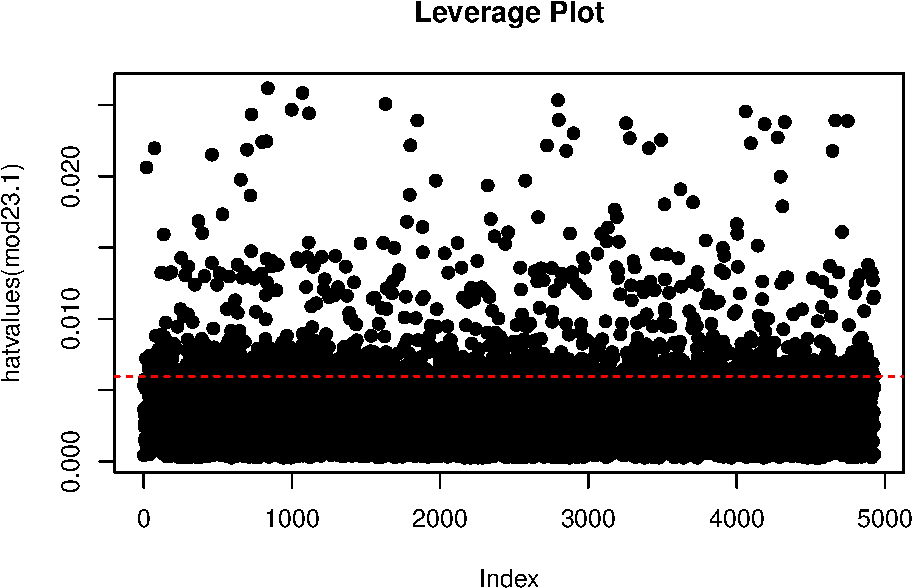
\includegraphics{Assigment2_files/figure-latex/unnamed-chunk-77-1.pdf}

We have more influential data than before, 399 tuples. We see that they
are distributed randomly. We consider to not delete this data because it
gives us important information for the model.

\hypertarget{residuals-1}{%
\subsubsection{Residuals}\label{residuals-1}}

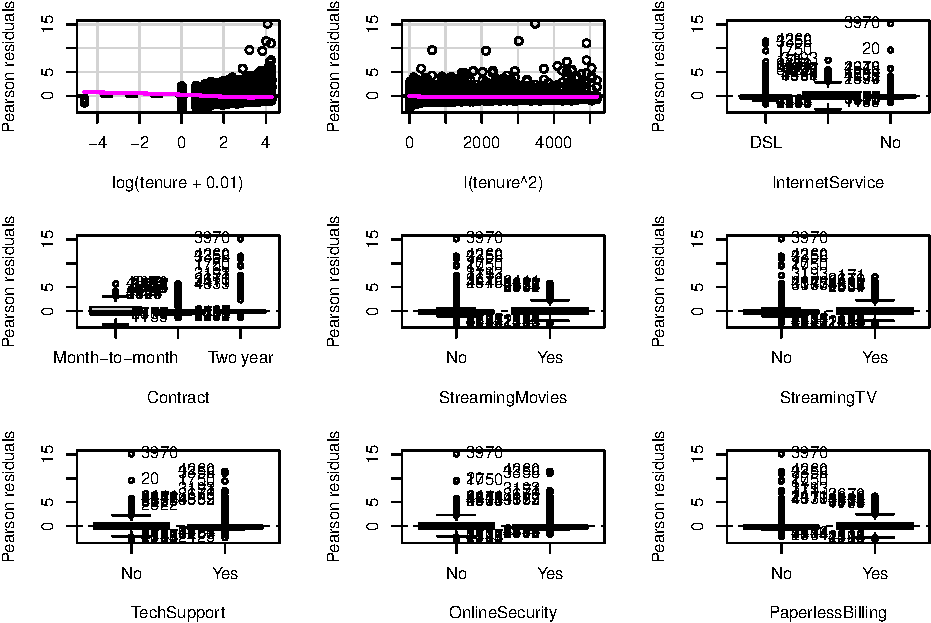
\includegraphics{Assigment2_files/figure-latex/unnamed-chunk-78-1.pdf}
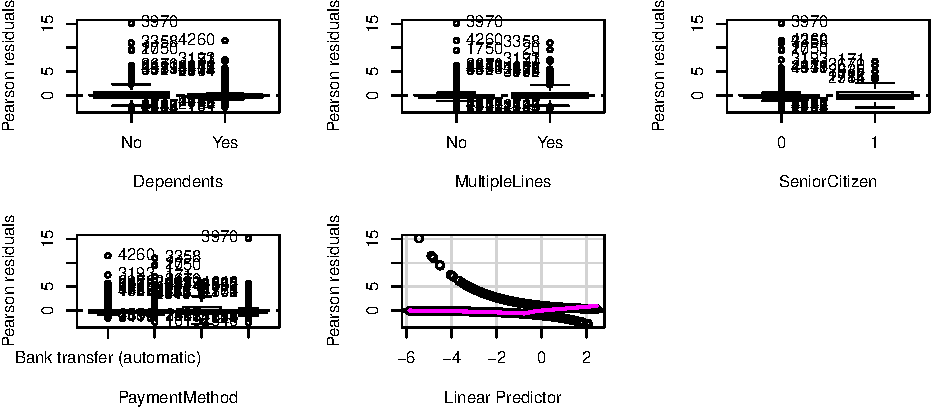
\includegraphics{Assigment2_files/figure-latex/unnamed-chunk-78-2.pdf}

\begin{verbatim}
##                    Test stat Pr(>|Test stat|)   
## log(tenure + 0.01)    7.0074         0.008117 **
## I(tenure^2)           0.4388         0.507725   
## InternetService                                 
## Contract                                        
## StreamingMovies                                 
## StreamingTV                                     
## TechSupport                                     
## OnlineSecurity                                  
## PaperlessBilling                                
## Dependents                                      
## MultipleLines                                   
## SeniorCitizen                                   
## PaymentMethod                                   
## ---
## Signif. codes:  0 '***' 0.001 '**' 0.01 '*' 0.05 '.' 0.1 ' ' 1
\end{verbatim}

We see that we have improved the residuals of the model. We can observe
that we have homoscedasticity because they are randomly distributed
considering that the model is binary.

\hypertarget{predictions}{%
\subsubsection{Predictions}\label{predictions}}

\begin{Shaded}
\begin{Highlighting}[]
\CommentTok{\#selecting the parameters that we have in the model}
\CommentTok{\#test\_data \textless{}{-} test[c(3,5,6,8,9,10,13,14,15,16,17,18)]}
\NormalTok{pred\_prob }\OtherTok{\textless{}{-}} \FunctionTok{predict}\NormalTok{(mod23}\FloatTok{.4}\NormalTok{, }\AttributeTok{newdata =}\NormalTok{ test, }\AttributeTok{type=}\StringTok{"response"}\NormalTok{)}
\NormalTok{churn\_pred}\OtherTok{\textless{}{-}} \FunctionTok{ifelse}\NormalTok{(pred\_prob}\SpecialCharTok{\textgreater{}}\FloatTok{0.5}\NormalTok{,}\StringTok{"Yes"}\NormalTok{,}\StringTok{"No"}\NormalTok{)}
\FunctionTok{table}\NormalTok{(churn\_pred)}
\end{Highlighting}
\end{Shaded}

\begin{verbatim}
## churn_pred
##   No  Yes 
## 1677  436
\end{verbatim}

\begin{Shaded}
\begin{Highlighting}[]
\FunctionTok{table}\NormalTok{(test}\SpecialCharTok{$}\NormalTok{Churn)}
\end{Highlighting}
\end{Shaded}

\begin{verbatim}
## 
##   No  Yes 
## 1547  566
\end{verbatim}

\begin{Shaded}
\begin{Highlighting}[]
\CommentTok{\#Confusion table}
\NormalTok{tt }\OtherTok{\textless{}{-}} \FunctionTok{table}\NormalTok{(churn\_pred, test}\SpecialCharTok{$}\NormalTok{Churn);tt}
\end{Highlighting}
\end{Shaded}

\begin{verbatim}
##           
## churn_pred   No  Yes
##        No  1409  268
##        Yes  138  298
\end{verbatim}

\begin{Shaded}
\begin{Highlighting}[]
\DecValTok{100}\SpecialCharTok{*}\FunctionTok{sum}\NormalTok{(}\FunctionTok{diag}\NormalTok{(tt))}\SpecialCharTok{/}\FunctionTok{sum}\NormalTok{(tt) }\CommentTok{\#80.79}
\end{Highlighting}
\end{Shaded}

\begin{verbatim}
## [1] 80.78561
\end{verbatim}

The accuracy of our model is good, it is \(80.79%
\).

\begin{Shaded}
\begin{Highlighting}[]
\NormalTok{roc\_curve }\OtherTok{\textless{}{-}} \FunctionTok{roc}\NormalTok{(test}\SpecialCharTok{$}\NormalTok{Churn, pred\_prob)}
\end{Highlighting}
\end{Shaded}

\begin{verbatim}
## Setting levels: control = No, case = Yes
\end{verbatim}

\begin{verbatim}
## Setting direction: controls < cases
\end{verbatim}

\begin{Shaded}
\begin{Highlighting}[]
\CommentTok{\# Plot the ROC curve}
\FunctionTok{plot}\NormalTok{(roc\_curve, }\AttributeTok{main =} \StringTok{"ROC Curve"}\NormalTok{, }\AttributeTok{col =} \StringTok{"blue"}\NormalTok{, }\AttributeTok{lwd =} \DecValTok{2}\NormalTok{)}
\CommentTok{\# Add diagonal reference line for comparison}
\FunctionTok{abline}\NormalTok{(}\AttributeTok{a =} \DecValTok{0}\NormalTok{, }\AttributeTok{b =} \DecValTok{1}\NormalTok{, }\AttributeTok{lty =} \DecValTok{2}\NormalTok{, }\AttributeTok{col =} \StringTok{"red"}\NormalTok{)}
\CommentTok{\# Add AUC (Area Under the Curve) value to the plot}
\FunctionTok{text}\NormalTok{(}\FloatTok{0.8}\NormalTok{, }\FloatTok{0.2}\NormalTok{, }\FunctionTok{paste}\NormalTok{(}\StringTok{"AUC ="}\NormalTok{, }\FunctionTok{round}\NormalTok{(}\FunctionTok{auc}\NormalTok{(roc\_curve), }\DecValTok{2}\NormalTok{)), }\AttributeTok{col =} \StringTok{"blue"}\NormalTok{, }\AttributeTok{cex =} \FloatTok{1.2}\NormalTok{)}
\end{Highlighting}
\end{Shaded}

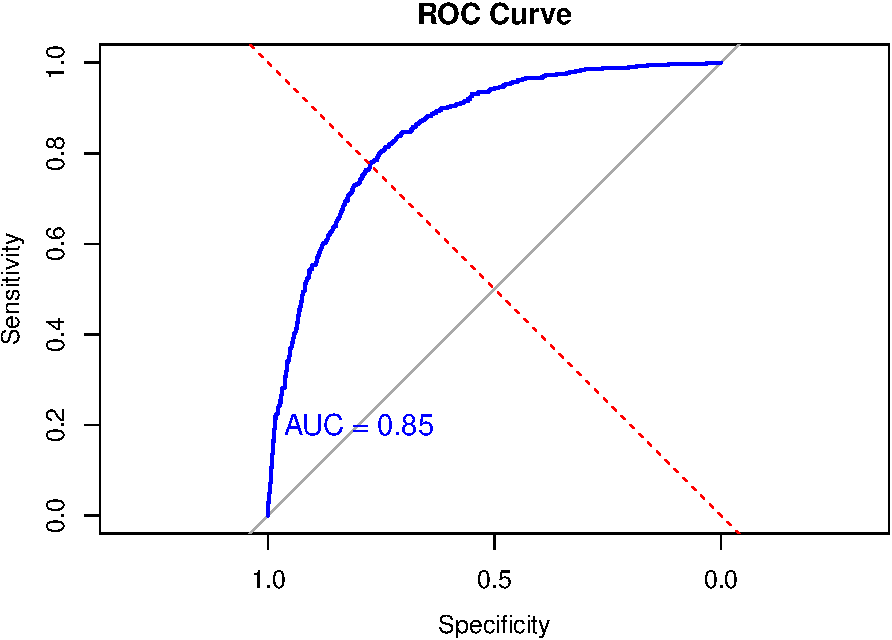
\includegraphics{Assigment2_files/figure-latex/unnamed-chunk-80-1.pdf}

Our Area Under the Curve for ROC curve is 0.85 so it is high.

\#Interpretation

\hypertarget{final-model}{%
\subsection{Final Model}\label{final-model}}

Our \textbf{final model} is:

\[
\begin{aligned}
Y &= -0.58 - 0.5 \cdot log(\text{tenure}+0.01) + 0.00005 \cdot \text{tenure}^2 \\
&\quad + 0.54 \cdot \text{InternetServiceFiber optic} - 0.97 \cdot \text{InternetServiceNo} \\
&\quad - 0.75 \cdot \text{ContractOne year} - 1.90 \cdot \text{ContractTwo year} \\
&\quad + 0.26 \cdot \text{StreamingMoviesYes} + 0.33 \cdot \text{StreamingTVYes} \\
&\quad - 0.22 \cdot \text{TechSupportYes} - 0.28 \cdot \text{Online SecurityYes} \\
&\quad + 0.33 \cdot \text{PaperlessBillingYes} - 0.23 \cdot \text{DependentsYes} \\
&\quad + 0.32 \cdot \text{MultipleLinesYes} - 0.15 \cdot \text{SeniorCitizen1} \\
&\quad - 0.25 \cdot \text{PaymentMethodCredit card} + 0.27 \cdot \text{PaymentMethodElectronic check} \\
&\quad - 0.25 \cdot \text{PaymentMethodMailed check} \\
&\quad + 0.87 \cdot \text{SeniorCitizen1:PaymentMethodCredit card} \\
&\quad + 0.28 \cdot \text{SeniorCitizen1: PaymentMethodElectronic check} \\
&\quad + 1.10 \cdot \text{SeniorCitizen1:PaymentMethodMailed check}
\end{aligned}
\]

\newpage

\hypertarget{annex}{%
\section{Annex}\label{annex}}

\hypertarget{univariate}{%
\subsection{Univariate}\label{univariate}}

\begin{Shaded}
\begin{Highlighting}[]
\FunctionTok{names}\NormalTok{(train)}
\end{Highlighting}
\end{Shaded}

\begin{verbatim}
##  [1] "customerID"       "gender"           "SeniorCitizen"    "Partner"         
##  [5] "Dependents"       "tenure"           "PhoneService"     "MultipleLines"   
##  [9] "InternetService"  "OnlineSecurity"   "OnlineBackup"     "DeviceProtection"
## [13] "TechSupport"      "StreamingTV"      "StreamingMovies"  "Contract"        
## [17] "PaperlessBilling" "PaymentMethod"    "MonthlyCharges"   "TotalCharges"    
## [21] "Churn"
\end{verbatim}

\begin{Shaded}
\begin{Highlighting}[]
\NormalTok{mod }\OtherTok{\textless{}{-}} \FunctionTok{glm}\NormalTok{(Churn }\SpecialCharTok{\textasciitilde{}}\NormalTok{ gender, }\AttributeTok{data=}\NormalTok{train, }\AttributeTok{family=}\NormalTok{binomial)}
\FunctionTok{summary}\NormalTok{(mod)}
\end{Highlighting}
\end{Shaded}

\begin{verbatim}
## 
## Call:
## glm(formula = Churn ~ gender, family = binomial, data = train)
## 
## Coefficients:
##             Estimate Std. Error z value Pr(>|z|)    
## (Intercept) -1.00637    0.04542 -22.158   <2e-16 ***
## genderMale  -0.03499    0.06460  -0.542    0.588    
## ---
## Signif. codes:  0 '***' 0.001 '**' 0.01 '*' 0.05 '.' 0.1 ' ' 1
## 
## (Dispersion parameter for binomial family taken to be 1)
## 
##     Null deviance: 5694.2  on 4929  degrees of freedom
## Residual deviance: 5693.9  on 4928  degrees of freedom
## AIC: 5697.9
## 
## Number of Fisher Scoring iterations: 4
\end{verbatim}

\begin{Shaded}
\begin{Highlighting}[]
\NormalTok{mod2 }\OtherTok{\textless{}{-}} \FunctionTok{glm}\NormalTok{(Churn }\SpecialCharTok{\textasciitilde{}}\NormalTok{ SeniorCitizen, }\AttributeTok{data=}\NormalTok{train, }\AttributeTok{family=}\NormalTok{binomial)}
\FunctionTok{summary}\NormalTok{(mod2)}
\end{Highlighting}
\end{Shaded}

\begin{verbatim}
## 
## Call:
## glm(formula = Churn ~ SeniorCitizen, family = binomial, data = train)
## 
## Coefficients:
##                Estimate Std. Error z value Pr(>|z|)    
## (Intercept)    -1.19026    0.03682  -32.33   <2e-16 ***
## SeniorCitizen1  0.88226    0.08027   10.99   <2e-16 ***
## ---
## Signif. codes:  0 '***' 0.001 '**' 0.01 '*' 0.05 '.' 0.1 ' ' 1
## 
## (Dispersion parameter for binomial family taken to be 1)
## 
##     Null deviance: 5694.2  on 4929  degrees of freedom
## Residual deviance: 5577.9  on 4928  degrees of freedom
## AIC: 5581.9
## 
## Number of Fisher Scoring iterations: 4
\end{verbatim}

\begin{Shaded}
\begin{Highlighting}[]
\NormalTok{mod3 }\OtherTok{\textless{}{-}} \FunctionTok{glm}\NormalTok{(Churn }\SpecialCharTok{\textasciitilde{}}\NormalTok{ Partner, }\AttributeTok{data=}\NormalTok{train, }\AttributeTok{family=}\NormalTok{binomial)}
\FunctionTok{summary}\NormalTok{(mod3)}
\end{Highlighting}
\end{Shaded}

\begin{verbatim}
## 
## Call:
## glm(formula = Churn ~ Partner, family = binomial, data = train)
## 
## Coefficients:
##             Estimate Std. Error z value Pr(>|z|)    
## (Intercept) -0.70909    0.04215  -16.82   <2e-16 ***
## PartnerYes  -0.71326    0.06676  -10.68   <2e-16 ***
## ---
## Signif. codes:  0 '***' 0.001 '**' 0.01 '*' 0.05 '.' 0.1 ' ' 1
## 
## (Dispersion parameter for binomial family taken to be 1)
## 
##     Null deviance: 5694.2  on 4929  degrees of freedom
## Residual deviance: 5576.5  on 4928  degrees of freedom
## AIC: 5580.5
## 
## Number of Fisher Scoring iterations: 4
\end{verbatim}

\begin{Shaded}
\begin{Highlighting}[]
\NormalTok{mod4 }\OtherTok{\textless{}{-}} \FunctionTok{glm}\NormalTok{(Churn }\SpecialCharTok{\textasciitilde{}}\NormalTok{ Dependents, }\AttributeTok{data=}\NormalTok{train, }\AttributeTok{family=}\NormalTok{binomial)}
\FunctionTok{summary}\NormalTok{(mod4)}
\end{Highlighting}
\end{Shaded}

\begin{verbatim}
## 
## Call:
## glm(formula = Churn ~ Dependents, family = binomial, data = train)
## 
## Coefficients:
##               Estimate Std. Error z value Pr(>|z|)    
## (Intercept)   -0.78158    0.03662  -21.34   <2e-16 ***
## DependentsYes -0.97564    0.08228  -11.86   <2e-16 ***
## ---
## Signif. codes:  0 '***' 0.001 '**' 0.01 '*' 0.05 '.' 0.1 ' ' 1
## 
## (Dispersion parameter for binomial family taken to be 1)
## 
##     Null deviance: 5694.2  on 4929  degrees of freedom
## Residual deviance: 5534.9  on 4928  degrees of freedom
## AIC: 5538.9
## 
## Number of Fisher Scoring iterations: 4
\end{verbatim}

\begin{Shaded}
\begin{Highlighting}[]
\NormalTok{mod5 }\OtherTok{\textless{}{-}} \FunctionTok{glm}\NormalTok{(Churn }\SpecialCharTok{\textasciitilde{}}\NormalTok{ tenure, }\AttributeTok{data=}\NormalTok{train, }\AttributeTok{family=}\NormalTok{binomial)}
\FunctionTok{summary}\NormalTok{(mod5)}
\end{Highlighting}
\end{Shaded}

\begin{verbatim}
## 
## Call:
## glm(formula = Churn ~ tenure, family = binomial, data = train)
## 
## Coefficients:
##              Estimate Std. Error z value Pr(>|z|)    
## (Intercept)  0.010348   0.050517   0.205    0.838    
## tenure      -0.038339   0.001679 -22.837   <2e-16 ***
## ---
## Signif. codes:  0 '***' 0.001 '**' 0.01 '*' 0.05 '.' 0.1 ' ' 1
## 
## (Dispersion parameter for binomial family taken to be 1)
## 
##     Null deviance: 5694.2  on 4929  degrees of freedom
## Residual deviance: 5040.7  on 4928  degrees of freedom
## AIC: 5044.7
## 
## Number of Fisher Scoring iterations: 4
\end{verbatim}

\begin{Shaded}
\begin{Highlighting}[]
\NormalTok{mod6 }\OtherTok{\textless{}{-}} \FunctionTok{glm}\NormalTok{(Churn }\SpecialCharTok{\textasciitilde{}}\NormalTok{ PhoneService, }\AttributeTok{data=}\NormalTok{train, }\AttributeTok{family=}\NormalTok{binomial)}
\FunctionTok{summary}\NormalTok{(mod6)}
\end{Highlighting}
\end{Shaded}

\begin{verbatim}
## 
## Call:
## glm(formula = Churn ~ PhoneService, family = binomial, data = train)
## 
## Coefficients:
##                 Estimate Std. Error z value Pr(>|z|)    
## (Intercept)      -1.1415     0.1076 -10.611   <2e-16 ***
## PhoneServiceYes   0.1299     0.1128   1.151     0.25    
## ---
## Signif. codes:  0 '***' 0.001 '**' 0.01 '*' 0.05 '.' 0.1 ' ' 1
## 
## (Dispersion parameter for binomial family taken to be 1)
## 
##     Null deviance: 5694.2  on 4929  degrees of freedom
## Residual deviance: 5692.9  on 4928  degrees of freedom
## AIC: 5696.9
## 
## Number of Fisher Scoring iterations: 4
\end{verbatim}

\begin{Shaded}
\begin{Highlighting}[]
\NormalTok{mod7 }\OtherTok{\textless{}{-}} \FunctionTok{glm}\NormalTok{(Churn }\SpecialCharTok{\textasciitilde{}}\NormalTok{ MultipleLines, }\AttributeTok{data=}\NormalTok{train, }\AttributeTok{family=}\NormalTok{binomial)}
\FunctionTok{summary}\NormalTok{(mod7)}
\end{Highlighting}
\end{Shaded}

\begin{verbatim}
## 
## Call:
## glm(formula = Churn ~ MultipleLines, family = binomial, data = train)
## 
## Coefficients:
##                  Estimate Std. Error z value Pr(>|z|)    
## (Intercept)      -1.12350    0.04348 -25.841  < 2e-16 ***
## MultipleLinesYes  0.23006    0.06505   3.537 0.000405 ***
## ---
## Signif. codes:  0 '***' 0.001 '**' 0.01 '*' 0.05 '.' 0.1 ' ' 1
## 
## (Dispersion parameter for binomial family taken to be 1)
## 
##     Null deviance: 5694.2  on 4929  degrees of freedom
## Residual deviance: 5681.7  on 4928  degrees of freedom
## AIC: 5685.7
## 
## Number of Fisher Scoring iterations: 4
\end{verbatim}

\begin{Shaded}
\begin{Highlighting}[]
\NormalTok{mod8 }\OtherTok{\textless{}{-}} \FunctionTok{glm}\NormalTok{(Churn }\SpecialCharTok{\textasciitilde{}}\NormalTok{ InternetService, }\AttributeTok{data=}\NormalTok{train, }\AttributeTok{family=}\NormalTok{binomial)}
\FunctionTok{summary}\NormalTok{(mod8)}
\end{Highlighting}
\end{Shaded}

\begin{verbatim}
## 
## Call:
## glm(formula = Churn ~ InternetService, family = binomial, data = train)
## 
## Coefficients:
##                            Estimate Std. Error z value Pr(>|z|)    
## (Intercept)                -1.47098    0.06258 -23.506   <2e-16 ***
## InternetServiceFiber optic  1.13842    0.07611  14.957   <2e-16 ***
## InternetServiceNo          -1.11658    0.13582  -8.221   <2e-16 ***
## ---
## Signif. codes:  0 '***' 0.001 '**' 0.01 '*' 0.05 '.' 0.1 ' ' 1
## 
## (Dispersion parameter for binomial family taken to be 1)
## 
##     Null deviance: 5694.2  on 4929  degrees of freedom
## Residual deviance: 5132.9  on 4927  degrees of freedom
## AIC: 5138.9
## 
## Number of Fisher Scoring iterations: 5
\end{verbatim}

\begin{Shaded}
\begin{Highlighting}[]
\NormalTok{mod9 }\OtherTok{\textless{}{-}} \FunctionTok{glm}\NormalTok{(Churn }\SpecialCharTok{\textasciitilde{}}\NormalTok{ OnlineSecurity, }\AttributeTok{data=}\NormalTok{train, }\AttributeTok{family=}\NormalTok{binomial)}
\FunctionTok{summary}\NormalTok{(mod9)}
\end{Highlighting}
\end{Shaded}

\begin{verbatim}
## 
## Call:
## glm(formula = Churn ~ OnlineSecurity, family = binomial, data = train)
## 
## Coefficients:
##                   Estimate Std. Error z value Pr(>|z|)    
## (Intercept)       -0.79719    0.03633  -21.94   <2e-16 ***
## OnlineSecurityYes -0.96472    0.08405  -11.48   <2e-16 ***
## ---
## Signif. codes:  0 '***' 0.001 '**' 0.01 '*' 0.05 '.' 0.1 ' ' 1
## 
## (Dispersion parameter for binomial family taken to be 1)
## 
##     Null deviance: 5694.2  on 4929  degrees of freedom
## Residual deviance: 5544.3  on 4928  degrees of freedom
## AIC: 5548.3
## 
## Number of Fisher Scoring iterations: 4
\end{verbatim}

\begin{Shaded}
\begin{Highlighting}[]
\NormalTok{mod10 }\OtherTok{\textless{}{-}} \FunctionTok{glm}\NormalTok{(Churn }\SpecialCharTok{\textasciitilde{}}\NormalTok{ OnlineBackup, }\AttributeTok{data=}\NormalTok{train, }\AttributeTok{family=}\NormalTok{binomial)}
\FunctionTok{summary}\NormalTok{(mod10)}
\end{Highlighting}
\end{Shaded}

\begin{verbatim}
## 
## Call:
## glm(formula = Churn ~ OnlineBackup, family = binomial, data = train)
## 
## Coefficients:
##                 Estimate Std. Error z value Pr(>|z|)    
## (Intercept)     -0.91109    0.03891 -23.414  < 2e-16 ***
## OnlineBackupYes -0.34507    0.07016  -4.919 8.72e-07 ***
## ---
## Signif. codes:  0 '***' 0.001 '**' 0.01 '*' 0.05 '.' 0.1 ' ' 1
## 
## (Dispersion parameter for binomial family taken to be 1)
## 
##     Null deviance: 5694.2  on 4929  degrees of freedom
## Residual deviance: 5669.4  on 4928  degrees of freedom
## AIC: 5673.4
## 
## Number of Fisher Scoring iterations: 4
\end{verbatim}

\begin{Shaded}
\begin{Highlighting}[]
\NormalTok{mod11 }\OtherTok{\textless{}{-}} \FunctionTok{glm}\NormalTok{(Churn }\SpecialCharTok{\textasciitilde{}}\NormalTok{ DeviceProtection, }\AttributeTok{data=}\NormalTok{train, }\AttributeTok{family=}\NormalTok{binomial)}
\FunctionTok{summary}\NormalTok{(mod11)}
\end{Highlighting}
\end{Shaded}

\begin{verbatim}
## 
## Call:
## glm(formula = Churn ~ DeviceProtection, family = binomial, data = train)
## 
## Coefficients:
##                     Estimate Std. Error z value Pr(>|z|)    
## (Intercept)         -0.93239    0.03909 -23.852  < 2e-16 ***
## DeviceProtectionYes -0.27669    0.06963  -3.973 7.09e-05 ***
## ---
## Signif. codes:  0 '***' 0.001 '**' 0.01 '*' 0.05 '.' 0.1 ' ' 1
## 
## (Dispersion parameter for binomial family taken to be 1)
## 
##     Null deviance: 5694.2  on 4929  degrees of freedom
## Residual deviance: 5678.1  on 4928  degrees of freedom
## AIC: 5682.1
## 
## Number of Fisher Scoring iterations: 4
\end{verbatim}

\begin{Shaded}
\begin{Highlighting}[]
\NormalTok{mod12 }\OtherTok{\textless{}{-}} \FunctionTok{glm}\NormalTok{(Churn }\SpecialCharTok{\textasciitilde{}}\NormalTok{ TechSupport, }\AttributeTok{data=}\NormalTok{train, }\AttributeTok{family=}\NormalTok{binomial)}
\FunctionTok{summary}\NormalTok{(mod12)}
\end{Highlighting}
\end{Shaded}

\begin{verbatim}
## 
## Call:
## glm(formula = Churn ~ TechSupport, family = binomial, data = train)
## 
## Coefficients:
##                Estimate Std. Error z value Pr(>|z|)    
## (Intercept)    -0.80594    0.03674  -21.94   <2e-16 ***
## TechSupportYes -0.86397    0.08058  -10.72   <2e-16 ***
## ---
## Signif. codes:  0 '***' 0.001 '**' 0.01 '*' 0.05 '.' 0.1 ' ' 1
## 
## (Dispersion parameter for binomial family taken to be 1)
## 
##     Null deviance: 5694.2  on 4929  degrees of freedom
## Residual deviance: 5566.6  on 4928  degrees of freedom
## AIC: 5570.6
## 
## Number of Fisher Scoring iterations: 4
\end{verbatim}

\begin{Shaded}
\begin{Highlighting}[]
\NormalTok{mod13 }\OtherTok{\textless{}{-}} \FunctionTok{glm}\NormalTok{(Churn }\SpecialCharTok{\textasciitilde{}}\NormalTok{ StreamingTV, }\AttributeTok{data=}\NormalTok{train, }\AttributeTok{family=}\NormalTok{binomial)}
\FunctionTok{summary}\NormalTok{(mod13)}
\end{Highlighting}
\end{Shaded}

\begin{verbatim}
## 
## Call:
## glm(formula = Churn ~ StreamingTV, family = binomial, data = train)
## 
## Coefficients:
##                Estimate Std. Error z value Pr(>|z|)    
## (Intercept)    -1.14795    0.04263 -26.931  < 2e-16 ***
## StreamingTVYes  0.30561    0.06551   4.665 3.09e-06 ***
## ---
## Signif. codes:  0 '***' 0.001 '**' 0.01 '*' 0.05 '.' 0.1 ' ' 1
## 
## (Dispersion parameter for binomial family taken to be 1)
## 
##     Null deviance: 5694.2  on 4929  degrees of freedom
## Residual deviance: 5672.6  on 4928  degrees of freedom
## AIC: 5676.6
## 
## Number of Fisher Scoring iterations: 4
\end{verbatim}

\begin{Shaded}
\begin{Highlighting}[]
\NormalTok{mod14 }\OtherTok{\textless{}{-}} \FunctionTok{glm}\NormalTok{(Churn }\SpecialCharTok{\textasciitilde{}}\NormalTok{ StreamingMovies, }\AttributeTok{data=}\NormalTok{train, }\AttributeTok{family=}\NormalTok{binomial)}
\FunctionTok{summary}\NormalTok{(mod14)}
\end{Highlighting}
\end{Shaded}

\begin{verbatim}
## 
## Call:
## glm(formula = Churn ~ StreamingMovies, family = binomial, data = train)
## 
## Coefficients:
##                    Estimate Std. Error z value Pr(>|z|)    
## (Intercept)        -1.12512    0.04254 -26.449  < 2e-16 ***
## StreamingMoviesYes  0.24849    0.06550   3.794 0.000148 ***
## ---
## Signif. codes:  0 '***' 0.001 '**' 0.01 '*' 0.05 '.' 0.1 ' ' 1
## 
## (Dispersion parameter for binomial family taken to be 1)
## 
##     Null deviance: 5694.2  on 4929  degrees of freedom
## Residual deviance: 5679.9  on 4928  degrees of freedom
## AIC: 5683.9
## 
## Number of Fisher Scoring iterations: 4
\end{verbatim}

\begin{Shaded}
\begin{Highlighting}[]
\NormalTok{mod15 }\OtherTok{\textless{}{-}} \FunctionTok{glm}\NormalTok{(Churn }\SpecialCharTok{\textasciitilde{}}\NormalTok{ Contract, }\AttributeTok{data=}\NormalTok{train, }\AttributeTok{family=}\NormalTok{binomial)}
\FunctionTok{summary}\NormalTok{(mod15)}
\end{Highlighting}
\end{Shaded}

\begin{verbatim}
## 
## Call:
## glm(formula = Churn ~ Contract, family = binomial, data = train)
## 
## Coefficients:
##                  Estimate Std. Error z value Pr(>|z|)    
## (Intercept)      -0.30975    0.03876  -7.992 1.33e-15 ***
## ContractOne year -1.73958    0.10521 -16.535  < 2e-16 ***
## ContractTwo year -3.29329    0.18611 -17.695  < 2e-16 ***
## ---
## Signif. codes:  0 '***' 0.001 '**' 0.01 '*' 0.05 '.' 0.1 ' ' 1
## 
## (Dispersion parameter for binomial family taken to be 1)
## 
##     Null deviance: 5694.2  on 4929  degrees of freedom
## Residual deviance: 4736.2  on 4927  degrees of freedom
## AIC: 4742.2
## 
## Number of Fisher Scoring iterations: 6
\end{verbatim}

\begin{Shaded}
\begin{Highlighting}[]
\NormalTok{mod16 }\OtherTok{\textless{}{-}} \FunctionTok{glm}\NormalTok{(Churn }\SpecialCharTok{\textasciitilde{}}\NormalTok{ PaperlessBilling, }\AttributeTok{data=}\NormalTok{train, }\AttributeTok{family=}\NormalTok{binomial)}
\FunctionTok{summary}\NormalTok{(mod16)}
\end{Highlighting}
\end{Shaded}

\begin{verbatim}
## 
## Call:
## glm(formula = Churn ~ PaperlessBilling, family = binomial, data = train)
## 
## Coefficients:
##                     Estimate Std. Error z value Pr(>|z|)    
## (Intercept)         -1.62562    0.06013  -27.04   <2e-16 ***
## PaperlessBillingYes  0.93196    0.07182   12.98   <2e-16 ***
## ---
## Signif. codes:  0 '***' 0.001 '**' 0.01 '*' 0.05 '.' 0.1 ' ' 1
## 
## (Dispersion parameter for binomial family taken to be 1)
## 
##     Null deviance: 5694.2  on 4929  degrees of freedom
## Residual deviance: 5512.4  on 4928  degrees of freedom
## AIC: 5516.4
## 
## Number of Fisher Scoring iterations: 4
\end{verbatim}

\begin{Shaded}
\begin{Highlighting}[]
\NormalTok{mod17 }\OtherTok{\textless{}{-}} \FunctionTok{glm}\NormalTok{(Churn }\SpecialCharTok{\textasciitilde{}}\NormalTok{ PaymentMethod, }\AttributeTok{data=}\NormalTok{train, }\AttributeTok{family=}\NormalTok{binomial)}
\FunctionTok{summary}\NormalTok{(mod17)}
\end{Highlighting}
\end{Shaded}

\begin{verbatim}
## 
## Call:
## glm(formula = Churn ~ PaymentMethod, family = binomial, data = train)
## 
## Coefficients:
##                                      Estimate Std. Error z value Pr(>|z|)    
## (Intercept)                          -1.59686    0.08266 -19.319   <2e-16 ***
## PaymentMethodCredit card (automatic) -0.15101    0.11847  -1.275    0.202    
## PaymentMethodElectronic check         1.40923    0.09627  14.638   <2e-16 ***
## PaymentMethodMailed check             0.13813    0.11233   1.230    0.219    
## ---
## Signif. codes:  0 '***' 0.001 '**' 0.01 '*' 0.05 '.' 0.1 ' ' 1
## 
## (Dispersion parameter for binomial family taken to be 1)
## 
##     Null deviance: 5694.2  on 4929  degrees of freedom
## Residual deviance: 5246.3  on 4926  degrees of freedom
## AIC: 5254.3
## 
## Number of Fisher Scoring iterations: 4
\end{verbatim}

\begin{Shaded}
\begin{Highlighting}[]
\NormalTok{mod18 }\OtherTok{\textless{}{-}} \FunctionTok{glm}\NormalTok{(Churn }\SpecialCharTok{\textasciitilde{}}\NormalTok{ MonthlyCharges, }\AttributeTok{data=}\NormalTok{train, }\AttributeTok{family=}\NormalTok{binomial)}
\FunctionTok{summary}\NormalTok{(mod18)}
\end{Highlighting}
\end{Shaded}

\begin{verbatim}
## 
## Call:
## glm(formula = Churn ~ MonthlyCharges, family = binomial, data = train)
## 
## Coefficients:
##                 Estimate Std. Error z value Pr(>|z|)    
## (Intercept)    -2.120267   0.090047  -23.55   <2e-16 ***
## MonthlyCharges  0.016008   0.001166   13.73   <2e-16 ***
## ---
## Signif. codes:  0 '***' 0.001 '**' 0.01 '*' 0.05 '.' 0.1 ' ' 1
## 
## (Dispersion parameter for binomial family taken to be 1)
## 
##     Null deviance: 5694.2  on 4929  degrees of freedom
## Residual deviance: 5491.4  on 4928  degrees of freedom
## AIC: 5495.4
## 
## Number of Fisher Scoring iterations: 4
\end{verbatim}

\begin{Shaded}
\begin{Highlighting}[]
\NormalTok{mod19 }\OtherTok{\textless{}{-}} \FunctionTok{glm}\NormalTok{(Churn }\SpecialCharTok{\textasciitilde{}}\NormalTok{ TotalCharges, }\AttributeTok{data=}\NormalTok{train, }\AttributeTok{family=}\NormalTok{binomial)}
\FunctionTok{summary}\NormalTok{(mod19)}
\end{Highlighting}
\end{Shaded}

\begin{verbatim}
## 
## Call:
## glm(formula = Churn ~ TotalCharges, family = binomial, data = train)
## 
## Coefficients:
##                Estimate Std. Error z value Pr(>|z|)    
## (Intercept)  -5.713e-01  4.451e-02  -12.84   <2e-16 ***
## TotalCharges -2.257e-04  1.726e-05  -13.07   <2e-16 ***
## ---
## Signif. codes:  0 '***' 0.001 '**' 0.01 '*' 0.05 '.' 0.1 ' ' 1
## 
## (Dispersion parameter for binomial family taken to be 1)
## 
##     Null deviance: 5694.2  on 4929  degrees of freedom
## Residual deviance: 5494.9  on 4928  degrees of freedom
## AIC: 5498.9
## 
## Number of Fisher Scoring iterations: 4
\end{verbatim}

\begin{Shaded}
\begin{Highlighting}[]
\FunctionTok{AIC}\NormalTok{(mod, mod1,mod2,mod3,mod4,mod5,mod6,mod7,mod8,mod9,mod10,mod11,mod12, mod13,mod14)}
\end{Highlighting}
\end{Shaded}

\begin{verbatim}
##       df      AIC
## mod    2 5697.925
## mod1   2 5044.677
## mod2   2 5581.910
## mod3   2 5580.505
## mod4   2 5538.857
## mod5   2 5044.677
## mod6   2 5696.868
## mod7   2 5685.746
## mod8   3 5138.946
## mod9   2 5548.342
## mod10  2 5673.442
## mod11  2 5682.144
## mod12  2 5570.586
## mod13  2 5676.581
## mod14  2 5683.895
\end{verbatim}

\hypertarget{balanced-data}{%
\subsection{Balanced data}\label{balanced-data}}

If we calculate other metrics, we can see that our model has not a very
good precision, recall or f1 score.

\begin{Shaded}
\begin{Highlighting}[]
\NormalTok{true\_positives }\OtherTok{\textless{}{-}}\NormalTok{ tt[}\DecValTok{2}\NormalTok{, }\DecValTok{2}\NormalTok{]}
\NormalTok{false\_positives }\OtherTok{\textless{}{-}}\NormalTok{ tt[}\DecValTok{1}\NormalTok{, }\DecValTok{2}\NormalTok{]}
\NormalTok{false\_negatives }\OtherTok{\textless{}{-}}\NormalTok{ tt[}\DecValTok{2}\NormalTok{, }\DecValTok{1}\NormalTok{]}
\NormalTok{precision }\OtherTok{\textless{}{-}}\NormalTok{ true\_positives }\SpecialCharTok{/}\NormalTok{ (true\_positives }\SpecialCharTok{+}\NormalTok{ false\_positives)}
\NormalTok{precision}
\end{Highlighting}
\end{Shaded}

\begin{verbatim}
## [1] 0.5265018
\end{verbatim}

\begin{Shaded}
\begin{Highlighting}[]
\CommentTok{\# Recall}
\NormalTok{recall }\OtherTok{\textless{}{-}}\NormalTok{ true\_positives }\SpecialCharTok{/}\NormalTok{ (true\_positives }\SpecialCharTok{+}\NormalTok{ false\_negatives)}
\NormalTok{recall}
\end{Highlighting}
\end{Shaded}

\begin{verbatim}
## [1] 0.6834862
\end{verbatim}

\begin{Shaded}
\begin{Highlighting}[]
\CommentTok{\# F1 Score}
\NormalTok{f1\_score }\OtherTok{\textless{}{-}} \DecValTok{2} \SpecialCharTok{*}\NormalTok{ (precision }\SpecialCharTok{*}\NormalTok{ recall) }\SpecialCharTok{/}\NormalTok{ (precision }\SpecialCharTok{+}\NormalTok{ recall)}
\NormalTok{f1\_score}
\end{Highlighting}
\end{Shaded}

\begin{verbatim}
## [1] 0.5948104
\end{verbatim}

We could try to balance the target variable and see if there is any
improvement. To do that we will not do a mechanic stepwise, we will use
an authomatic step.

\begin{Shaded}
\begin{Highlighting}[]
\FunctionTok{table}\NormalTok{(train}\SpecialCharTok{$}\NormalTok{Churn)}
\end{Highlighting}
\end{Shaded}

\begin{verbatim}
## 
##   No  Yes 
## 3627 1303
\end{verbatim}

\begin{Shaded}
\begin{Highlighting}[]
\NormalTok{data\_balanced\_over }\OtherTok{\textless{}{-}} \FunctionTok{ovun.sample}\NormalTok{(Churn }\SpecialCharTok{\textasciitilde{}}\NormalTok{ ., }\AttributeTok{data =}\NormalTok{ train, }\AttributeTok{method =} \StringTok{"over"}\NormalTok{,}\AttributeTok{N=}\DecValTok{3627}\SpecialCharTok{*}\DecValTok{2}\NormalTok{)}\SpecialCharTok{$}\NormalTok{data}
\FunctionTok{table}\NormalTok{(data\_balanced\_over}\SpecialCharTok{$}\NormalTok{Churn)}
\end{Highlighting}
\end{Shaded}

\begin{verbatim}
## 
##   No  Yes 
## 3627 3627
\end{verbatim}

\begin{Shaded}
\begin{Highlighting}[]
\NormalTok{data\_balanced\_under }\OtherTok{\textless{}{-}} \FunctionTok{ovun.sample}\NormalTok{(Churn }\SpecialCharTok{\textasciitilde{}}\NormalTok{ ., }\AttributeTok{data =}\NormalTok{ train, }\AttributeTok{method =} \StringTok{"under"}\NormalTok{, }\AttributeTok{N =} \DecValTok{1303}\SpecialCharTok{*}\DecValTok{2}\NormalTok{, }\AttributeTok{seed =} \DecValTok{1}\NormalTok{)}\SpecialCharTok{$}\NormalTok{data}
\FunctionTok{table}\NormalTok{(data\_balanced\_under}\SpecialCharTok{$}\NormalTok{Churn)}
\end{Highlighting}
\end{Shaded}

\begin{verbatim}
## 
##   No  Yes 
## 1303 1303
\end{verbatim}

\hypertarget{with-undersampling}{%
\subsubsection{With undersampling}\label{with-undersampling}}

\begin{Shaded}
\begin{Highlighting}[]
\NormalTok{b0}\OtherTok{\textless{}{-}} \FunctionTok{glm}\NormalTok{(}
\NormalTok{  Churn }\SpecialCharTok{\textasciitilde{}} \FunctionTok{log}\NormalTok{(tenure }\SpecialCharTok{+} \FloatTok{0.01}\NormalTok{)}
  \SpecialCharTok{+}\NormalTok{ MonthlyCharges}
  \SpecialCharTok{+} \FunctionTok{log}\NormalTok{(TotalCharges }\SpecialCharTok{+} \FloatTok{0.01}\NormalTok{)}
  \SpecialCharTok{+}\NormalTok{ Contract }\SpecialCharTok{+}\NormalTok{ OnlineSecurity }\SpecialCharTok{+}\NormalTok{ TechSupport }\SpecialCharTok{+}\NormalTok{ InternetService }\SpecialCharTok{+}\NormalTok{ PaymentMethod }
  \SpecialCharTok{+}\NormalTok{ OnlineBackup }\SpecialCharTok{+}\NormalTok{ MultipleLines }\SpecialCharTok{+}\NormalTok{ PaperlessBilling }\SpecialCharTok{+}\NormalTok{ SeniorCitizen }\SpecialCharTok{+}\NormalTok{ Partner }
  \SpecialCharTok{+}\NormalTok{ gender }\SpecialCharTok{+}\NormalTok{ DeviceProtection }\SpecialCharTok{+}\NormalTok{ StreamingMovies }\SpecialCharTok{+}\NormalTok{ StreamingTV }\SpecialCharTok{+}\NormalTok{ PhoneService }
  \SpecialCharTok{+}\NormalTok{ Dependents,}
  \AttributeTok{data =}\NormalTok{ data\_balanced\_under,}
  \AttributeTok{family =}\NormalTok{ binomial}
\NormalTok{)}
\NormalTok{mod.fow }\OtherTok{\textless{}{-}}\NormalTok{ stats}\SpecialCharTok{::}\FunctionTok{step}\NormalTok{(b0, }\AttributeTok{trace =} \DecValTok{0}\NormalTok{, }\AttributeTok{direction =} \StringTok{"forward"}\NormalTok{)}
\FunctionTok{summary}\NormalTok{(mod.fow)}
\end{Highlighting}
\end{Shaded}

\begin{verbatim}
## 
## Call:
## glm(formula = Churn ~ log(tenure + 0.01) + MonthlyCharges + log(TotalCharges + 
##     0.01) + Contract + OnlineSecurity + TechSupport + InternetService + 
##     PaymentMethod + OnlineBackup + MultipleLines + PaperlessBilling + 
##     SeniorCitizen + Partner + gender + DeviceProtection + StreamingMovies + 
##     StreamingTV + PhoneService + Dependents, family = binomial, 
##     data = data_balanced_under)
## 
## Coefficients:
##                                      Estimate Std. Error z value Pr(>|z|)    
## (Intercept)                           1.02610    1.74560   0.588 0.556651    
## log(tenure + 0.01)                   -1.57060    0.40763  -3.853 0.000117 ***
## MonthlyCharges                       -0.09491    0.04889  -1.941 0.052233 .  
## log(TotalCharges + 0.01)              0.88270    0.38746   2.278 0.022718 *  
## ContractOne year                     -0.73559    0.15086  -4.876 1.08e-06 ***
## ContractTwo year                     -1.80639    0.23231  -7.776 7.50e-15 ***
## OnlineSecurityYes                     0.13082    0.27329   0.479 0.632172    
## TechSupportYes                        0.21153    0.27372   0.773 0.439631    
## InternetServiceFiber optic            2.95241    1.23064   2.399 0.016436 *  
## InternetServiceNo                    -2.55736    1.26511  -2.021 0.043233 *  
## PaymentMethodCredit card (automatic) -0.04210    0.16553  -0.254 0.799251    
## PaymentMethodElectronic check         0.39965    0.14389   2.778 0.005477 ** 
## PaymentMethodMailed check            -0.18360    0.17353  -1.058 0.290036    
## OnlineBackupYes                       0.49872    0.27161   1.836 0.066329 .  
## MultipleLinesYes                      0.81355    0.27466   2.962 0.003056 ** 
## PaperlessBillingYes                   0.22450    0.11533   1.947 0.051578 .  
## SeniorCitizen1                        0.37683    0.13549   2.781 0.005414 ** 
## PartnerYes                           -0.02618    0.11895  -0.220 0.825811    
## genderMale                           -0.02626    0.10176  -0.258 0.796358    
## DeviceProtectionYes                   0.47111    0.27341   1.723 0.084874 .  
## StreamingMoviesYes                    0.99992    0.50330   1.987 0.046952 *  
## StreamingTVYes                        1.19817    0.50457   2.375 0.017566 *  
## PhoneServiceYes                       1.05024    1.00774   1.042 0.297332    
## DependentsYes                        -0.19143    0.13424  -1.426 0.153862    
## ---
## Signif. codes:  0 '***' 0.001 '**' 0.01 '*' 0.05 '.' 0.1 ' ' 1
## 
## (Dispersion parameter for binomial family taken to be 1)
## 
##     Null deviance: 3612.7  on 2605  degrees of freedom
## Residual deviance: 2399.8  on 2582  degrees of freedom
## AIC: 2447.8
## 
## Number of Fisher Scoring iterations: 5
\end{verbatim}

\begin{Shaded}
\begin{Highlighting}[]
\NormalTok{b01}\OtherTok{\textless{}{-}} \FunctionTok{glm}\NormalTok{(}
\NormalTok{  Churn }\SpecialCharTok{\textasciitilde{}} \FunctionTok{log}\NormalTok{(tenure }\SpecialCharTok{+} \FloatTok{0.01}\NormalTok{)}
  \SpecialCharTok{+}\NormalTok{ MonthlyCharges}
  \SpecialCharTok{+} \FunctionTok{log}\NormalTok{(TotalCharges }\SpecialCharTok{+} \FloatTok{0.01}\NormalTok{)}
  \SpecialCharTok{+}\NormalTok{ Contract  }\SpecialCharTok{+}\NormalTok{ InternetService }\SpecialCharTok{+}\NormalTok{ PaymentMethod }
  \SpecialCharTok{+}\NormalTok{ OnlineBackup }\SpecialCharTok{+}\NormalTok{ MultipleLines }\SpecialCharTok{+}\NormalTok{ PaperlessBilling }\SpecialCharTok{+}\NormalTok{ SeniorCitizen  }
  \SpecialCharTok{+}\NormalTok{ DeviceProtection }\SpecialCharTok{+}\NormalTok{ StreamingMovies }\SpecialCharTok{+}\NormalTok{ StreamingTV,}
  \AttributeTok{data =}\NormalTok{ data\_balanced\_under,}
  \AttributeTok{family =}\NormalTok{ binomial}
\NormalTok{)}

\FunctionTok{summary}\NormalTok{(b01)}
\end{Highlighting}
\end{Shaded}

\begin{verbatim}
## 
## Call:
## glm(formula = Churn ~ log(tenure + 0.01) + MonthlyCharges + log(TotalCharges + 
##     0.01) + Contract + InternetService + PaymentMethod + OnlineBackup + 
##     MultipleLines + PaperlessBilling + SeniorCitizen + DeviceProtection + 
##     StreamingMovies + StreamingTV, family = binomial, data = data_balanced_under)
## 
## Coefficients:
##                                      Estimate Std. Error z value Pr(>|z|)    
## (Intercept)                          -0.45939    1.15789  -0.397 0.691551    
## log(tenure + 0.01)                   -1.70815    0.39589  -4.315 1.60e-05 ***
## MonthlyCharges                       -0.05156    0.01083  -4.760 1.94e-06 ***
## log(TotalCharges + 0.01)              1.00319    0.37811   2.653 0.007974 ** 
## ContractOne year                     -0.75932    0.14929  -5.086 3.65e-07 ***
## ContractTwo year                     -1.85424    0.22740  -8.154 3.51e-16 ***
## InternetServiceFiber optic            1.88349    0.27703   6.799 1.05e-11 ***
## InternetServiceNo                    -1.31324    0.29004  -4.528 5.96e-06 ***
## PaymentMethodCredit card (automatic) -0.04267    0.16501  -0.259 0.795934    
## PaymentMethodElectronic check         0.40902    0.14356   2.849 0.004385 ** 
## PaymentMethodMailed check            -0.17690    0.17261  -1.025 0.305418    
## OnlineBackupYes                       0.27307    0.12618   2.164 0.030457 *  
## MultipleLinesYes                      0.60906    0.13496   4.513 6.40e-06 ***
## PaperlessBillingYes                   0.23383    0.11479   2.037 0.041642 *  
## SeniorCitizen1                        0.41044    0.13284   3.090 0.002003 ** 
## DeviceProtectionYes                   0.24715    0.12587   1.964 0.049574 *  
## StreamingMoviesYes                    0.54993    0.14741   3.731 0.000191 ***
## StreamingTVYes                        0.74309    0.15138   4.909 9.17e-07 ***
## ---
## Signif. codes:  0 '***' 0.001 '**' 0.01 '*' 0.05 '.' 0.1 ' ' 1
## 
## (Dispersion parameter for binomial family taken to be 1)
## 
##     Null deviance: 3612.7  on 2605  degrees of freedom
## Residual deviance: 2404.4  on 2588  degrees of freedom
## AIC: 2440.4
## 
## Number of Fisher Scoring iterations: 5
\end{verbatim}

\begin{Shaded}
\begin{Highlighting}[]
\FunctionTok{vif}\NormalTok{(b01)}
\end{Highlighting}
\end{Shaded}

\begin{verbatim}
##                                GVIF Df GVIF^(1/(2*Df))
## log(tenure + 0.01)       108.431706  1       10.413055
## MonthlyCharges            35.834530  1        5.986195
## log(TotalCharges + 0.01) 158.334846  1       12.583118
## Contract                   1.549784  2        1.115752
## InternetService           17.126997  2        2.034325
## PaymentMethod              1.393533  3        1.056865
## OnlineBackup               1.436232  1        1.198429
## MultipleLines              1.763892  1        1.328116
## PaperlessBilling           1.141013  1        1.068182
## SeniorCitizen              1.070722  1        1.034757
## DeviceProtection           1.414452  1        1.189307
## StreamingMovies            2.101487  1        1.449651
## StreamingTV                2.201572  1        1.483770
\end{verbatim}

\begin{Shaded}
\begin{Highlighting}[]
\NormalTok{b02}\OtherTok{\textless{}{-}} \FunctionTok{glm}\NormalTok{(}
\NormalTok{  Churn }\SpecialCharTok{\textasciitilde{}} \FunctionTok{log}\NormalTok{(tenure }\SpecialCharTok{+} \FloatTok{0.01}\NormalTok{)}
  \SpecialCharTok{+}\NormalTok{ Contract  }\SpecialCharTok{+}\NormalTok{ InternetService }\SpecialCharTok{+}\NormalTok{ PaymentMethod }
  \SpecialCharTok{+}\NormalTok{ OnlineBackup }\SpecialCharTok{+}\NormalTok{ MultipleLines }\SpecialCharTok{+}\NormalTok{ PaperlessBilling }\SpecialCharTok{+}\NormalTok{ SeniorCitizen  }
  \SpecialCharTok{+}\NormalTok{ DeviceProtection }\SpecialCharTok{+}\NormalTok{ StreamingMovies }\SpecialCharTok{+}\NormalTok{ StreamingTV,}
  \AttributeTok{data =}\NormalTok{ data\_balanced\_under,}
  \AttributeTok{family =}\NormalTok{ binomial}
\NormalTok{)}
\FunctionTok{summary}\NormalTok{(b02)}
\end{Highlighting}
\end{Shaded}

\begin{verbatim}
## 
## Call:
## glm(formula = Churn ~ log(tenure + 0.01) + Contract + InternetService + 
##     PaymentMethod + OnlineBackup + MultipleLines + PaperlessBilling + 
##     SeniorCitizen + DeviceProtection + StreamingMovies + StreamingTV, 
##     family = binomial, data = data_balanced_under)
## 
## Coefficients:
##                                      Estimate Std. Error z value Pr(>|z|)    
## (Intercept)                           1.07661    0.19623   5.487 4.10e-08 ***
## log(tenure + 0.01)                   -0.67210    0.05355 -12.550  < 2e-16 ***
## ContractOne year                     -0.86956    0.14769  -5.888 3.92e-09 ***
## ContractTwo year                     -2.07880    0.22715  -9.152  < 2e-16 ***
## InternetServiceFiber optic            0.79059    0.12657   6.246 4.20e-10 ***
## InternetServiceNo                    -0.90842    0.19025  -4.775 1.80e-06 ***
## PaymentMethodCredit card (automatic) -0.03459    0.16407  -0.211  0.83303    
## PaymentMethodElectronic check         0.46124    0.14245   3.238  0.00120 ** 
## PaymentMethodMailed check            -0.16503    0.17167  -0.961  0.33636    
## OnlineBackupYes                       0.06474    0.11743   0.551  0.58139    
## MultipleLinesYes                      0.32700    0.11853   2.759  0.00580 ** 
## PaperlessBillingYes                   0.25980    0.11380   2.283  0.02243 *  
## SeniorCitizen1                        0.44926    0.13176   3.410  0.00065 ***
## DeviceProtectionYes                   0.05527    0.11864   0.466  0.64128    
## StreamingMoviesYes                    0.20328    0.12496   1.627  0.10380    
## StreamingTVYes                        0.36489    0.12652   2.884  0.00393 ** 
## ---
## Signif. codes:  0 '***' 0.001 '**' 0.01 '*' 0.05 '.' 0.1 ' ' 1
## 
## (Dispersion parameter for binomial family taken to be 1)
## 
##     Null deviance: 3612.7  on 2605  degrees of freedom
## Residual deviance: 2427.9  on 2590  degrees of freedom
## AIC: 2459.9
## 
## Number of Fisher Scoring iterations: 5
\end{verbatim}

\begin{Shaded}
\begin{Highlighting}[]
\FunctionTok{vif}\NormalTok{(b02)}
\end{Highlighting}
\end{Shaded}

\begin{verbatim}
##                        GVIF Df GVIF^(1/(2*Df))
## log(tenure + 0.01) 1.993586  1        1.411944
## Contract           1.484135  2        1.103744
## InternetService    1.803247  2        1.158814
## PaymentMethod      1.378311  3        1.054932
## OnlineBackup       1.259758  1        1.122389
## MultipleLines      1.378286  1        1.174004
## PaperlessBilling   1.132894  1        1.064375
## SeniorCitizen      1.063217  1        1.031124
## DeviceProtection   1.265955  1        1.125146
## StreamingMovies    1.526624  1        1.235566
## StreamingTV        1.554087  1        1.246630
\end{verbatim}

\begin{Shaded}
\begin{Highlighting}[]
\NormalTok{pred\_prob2 }\OtherTok{\textless{}{-}} \FunctionTok{predict}\NormalTok{(b02, }\AttributeTok{newdata =}\NormalTok{ test, }\AttributeTok{type=}\StringTok{"response"}\NormalTok{)}
\NormalTok{churn\_pred2}\OtherTok{\textless{}{-}} \FunctionTok{ifelse}\NormalTok{(pred\_prob2}\SpecialCharTok{\textgreater{}}\FloatTok{0.5}\NormalTok{,}\StringTok{"Yes"}\NormalTok{,}\StringTok{"No"}\NormalTok{)}
\FunctionTok{table}\NormalTok{(churn\_pred2)}
\end{Highlighting}
\end{Shaded}

\begin{verbatim}
## churn_pred2
##   No  Yes 
## 1259  854
\end{verbatim}

\begin{Shaded}
\begin{Highlighting}[]
\FunctionTok{table}\NormalTok{(test}\SpecialCharTok{$}\NormalTok{Churn)}
\end{Highlighting}
\end{Shaded}

\begin{verbatim}
## 
##   No  Yes 
## 1547  566
\end{verbatim}

\begin{Shaded}
\begin{Highlighting}[]
\CommentTok{\#Confusion table}
\NormalTok{tt2 }\OtherTok{\textless{}{-}} \FunctionTok{table}\NormalTok{(churn\_pred2, test}\SpecialCharTok{$}\NormalTok{Churn);tt}
\end{Highlighting}
\end{Shaded}

\begin{verbatim}
##           
## churn_pred   No  Yes
##        No  1409  268
##        Yes  138  298
\end{verbatim}

\begin{Shaded}
\begin{Highlighting}[]
\DecValTok{100}\SpecialCharTok{*}\FunctionTok{sum}\NormalTok{(}\FunctionTok{diag}\NormalTok{(tt2))}\SpecialCharTok{/}\FunctionTok{sum}\NormalTok{(tt2) }\CommentTok{\#80.79}
\end{Highlighting}
\end{Shaded}

\begin{verbatim}
## [1] 75.6744
\end{verbatim}

\begin{Shaded}
\begin{Highlighting}[]
\NormalTok{true\_positives }\OtherTok{\textless{}{-}}\NormalTok{ tt2[}\DecValTok{2}\NormalTok{, }\DecValTok{2}\NormalTok{]}
\NormalTok{false\_positives }\OtherTok{\textless{}{-}}\NormalTok{ tt2[}\DecValTok{1}\NormalTok{, }\DecValTok{2}\NormalTok{]}
\NormalTok{false\_negatives }\OtherTok{\textless{}{-}}\NormalTok{ tt2[}\DecValTok{2}\NormalTok{, }\DecValTok{1}\NormalTok{]}
\NormalTok{precision }\OtherTok{\textless{}{-}}\NormalTok{ true\_positives }\SpecialCharTok{/}\NormalTok{ (true\_positives }\SpecialCharTok{+}\NormalTok{ false\_positives)}
\NormalTok{precision}
\end{Highlighting}
\end{Shaded}

\begin{verbatim}
## [1] 0.8003534
\end{verbatim}

\begin{Shaded}
\begin{Highlighting}[]
\CommentTok{\# Recall}
\NormalTok{recall }\OtherTok{\textless{}{-}}\NormalTok{ true\_positives }\SpecialCharTok{/}\NormalTok{ (true\_positives }\SpecialCharTok{+}\NormalTok{ false\_negatives)}
\NormalTok{recall}
\end{Highlighting}
\end{Shaded}

\begin{verbatim}
## [1] 0.530445
\end{verbatim}

\begin{Shaded}
\begin{Highlighting}[]
\CommentTok{\# F1 Score}
\NormalTok{f1\_score }\OtherTok{\textless{}{-}} \DecValTok{2} \SpecialCharTok{*}\NormalTok{ (precision }\SpecialCharTok{*}\NormalTok{ recall) }\SpecialCharTok{/}\NormalTok{ (precision }\SpecialCharTok{+}\NormalTok{ recall)}
\NormalTok{f1\_score}
\end{Highlighting}
\end{Shaded}

\begin{verbatim}
## [1] 0.6380282
\end{verbatim}

\begin{Shaded}
\begin{Highlighting}[]
\NormalTok{b0}\OtherTok{\textless{}{-}} \FunctionTok{glm}\NormalTok{(}
\NormalTok{  Churn }\SpecialCharTok{\textasciitilde{}} \FunctionTok{log}\NormalTok{(tenure }\SpecialCharTok{+} \FloatTok{0.01}\NormalTok{)}
  \SpecialCharTok{+}\NormalTok{ MonthlyCharges}
  \SpecialCharTok{+} \FunctionTok{log}\NormalTok{(TotalCharges }\SpecialCharTok{+} \FloatTok{0.01}\NormalTok{)}
  \SpecialCharTok{+}\NormalTok{ Contract }\SpecialCharTok{+}\NormalTok{ OnlineSecurity }\SpecialCharTok{+}\NormalTok{ TechSupport }\SpecialCharTok{+}\NormalTok{ InternetService }\SpecialCharTok{+}\NormalTok{ PaymentMethod }
  \SpecialCharTok{+}\NormalTok{ OnlineBackup }\SpecialCharTok{+}\NormalTok{ MultipleLines }\SpecialCharTok{+}\NormalTok{ PaperlessBilling }\SpecialCharTok{+}\NormalTok{ SeniorCitizen }\SpecialCharTok{+}\NormalTok{ Partner }
  \SpecialCharTok{+}\NormalTok{ gender }\SpecialCharTok{+}\NormalTok{ DeviceProtection }\SpecialCharTok{+}\NormalTok{ StreamingMovies }\SpecialCharTok{+}\NormalTok{ StreamingTV }\SpecialCharTok{+}\NormalTok{ PhoneService }
  \SpecialCharTok{+}\NormalTok{ Dependents,}
  \AttributeTok{data =}\NormalTok{ data\_balanced\_over,}
  \AttributeTok{family =}\NormalTok{ binomial}
\NormalTok{)}
\NormalTok{mod.fow }\OtherTok{\textless{}{-}}\NormalTok{ stats}\SpecialCharTok{::}\FunctionTok{step}\NormalTok{(b0, }\AttributeTok{trace =} \DecValTok{0}\NormalTok{, }\AttributeTok{direction =} \StringTok{"forward"}\NormalTok{)}
\FunctionTok{summary}\NormalTok{(mod.fow)}
\end{Highlighting}
\end{Shaded}

\begin{verbatim}
## 
## Call:
## glm(formula = Churn ~ log(tenure + 0.01) + MonthlyCharges + log(TotalCharges + 
##     0.01) + Contract + OnlineSecurity + TechSupport + InternetService + 
##     PaymentMethod + OnlineBackup + MultipleLines + PaperlessBilling + 
##     SeniorCitizen + Partner + gender + DeviceProtection + StreamingMovies + 
##     StreamingTV + PhoneService + Dependents, family = binomial, 
##     data = data_balanced_over)
## 
## Coefficients:
##                                      Estimate Std. Error z value Pr(>|z|)    
## (Intercept)                           0.20915    0.96004   0.218 0.827543    
## log(tenure + 0.01)                   -1.63864    0.22345  -7.333 2.24e-13 ***
## MonthlyCharges                       -0.08689    0.02828  -3.072 0.002124 ** 
## log(TotalCharges + 0.01)              0.97214    0.21068   4.614 3.94e-06 ***
## ContractOne year                     -0.66701    0.08917  -7.480 7.42e-14 ***
## ContractTwo year                     -1.67592    0.13338 -12.565  < 2e-16 ***
## OnlineSecurityYes                     0.21666    0.15810   1.370 0.170550    
## TechSupportYes                        0.16724    0.15805   1.058 0.289991    
## InternetServiceFiber optic            2.75859    0.70943   3.888 0.000101 ***
## InternetServiceNo                    -2.25430    0.72493  -3.110 0.001873 ** 
## PaymentMethodCredit card (automatic) -0.09430    0.09717  -0.970 0.331806    
## PaymentMethodElectronic check         0.28641    0.08435   3.396 0.000685 ***
## PaymentMethodMailed check            -0.21656    0.10409  -2.081 0.037471 *  
## OnlineBackupYes                       0.44393    0.15679   2.831 0.004636 ** 
## MultipleLinesYes                      0.73334    0.16007   4.581 4.62e-06 ***
## PaperlessBillingYes                   0.28532    0.06854   4.163 3.14e-05 ***
## SeniorCitizen1                        0.23735    0.07902   3.004 0.002666 ** 
## PartnerYes                           -0.08161    0.07073  -1.154 0.248581    
## genderMale                            0.08603    0.06011   1.431 0.152335    
## DeviceProtectionYes                   0.43460    0.15719   2.765 0.005696 ** 
## StreamingMoviesYes                    1.00211    0.28974   3.459 0.000543 ***
## StreamingTVYes                        1.11520    0.29095   3.833 0.000127 ***
## PhoneServiceYes                       0.97936    0.57656   1.699 0.089389 .  
## DependentsYes                        -0.21480    0.08022  -2.678 0.007413 ** 
## ---
## Signif. codes:  0 '***' 0.001 '**' 0.01 '*' 0.05 '.' 0.1 ' ' 1
## 
## (Dispersion parameter for binomial family taken to be 1)
## 
##     Null deviance: 10056.2  on 7253  degrees of freedom
## Residual deviance:  6846.7  on 7230  degrees of freedom
## AIC: 6894.7
## 
## Number of Fisher Scoring iterations: 5
\end{verbatim}

\begin{Shaded}
\begin{Highlighting}[]
\NormalTok{b1}\OtherTok{\textless{}{-}} \FunctionTok{glm}\NormalTok{(}
\NormalTok{  Churn }\SpecialCharTok{\textasciitilde{}} \FunctionTok{log}\NormalTok{(tenure }\SpecialCharTok{+} \FloatTok{0.01}\NormalTok{)}
  \SpecialCharTok{+}\NormalTok{ MonthlyCharges}
  \SpecialCharTok{+} \FunctionTok{log}\NormalTok{(TotalCharges }\SpecialCharTok{+} \FloatTok{0.01}\NormalTok{)}
  \SpecialCharTok{+}\NormalTok{ Contract  }\SpecialCharTok{+}\NormalTok{ InternetService }\SpecialCharTok{+}\NormalTok{ PaymentMethod }
  \SpecialCharTok{+}\NormalTok{ OnlineBackup }\SpecialCharTok{+}\NormalTok{ MultipleLines }\SpecialCharTok{+}\NormalTok{ PaperlessBilling }\SpecialCharTok{+}\NormalTok{ SeniorCitizen }
   \SpecialCharTok{+}\NormalTok{ DeviceProtection }\SpecialCharTok{+}\NormalTok{ StreamingMovies }\SpecialCharTok{+}\NormalTok{ StreamingTV }
  \SpecialCharTok{+}\NormalTok{ Dependents,}
  \AttributeTok{data =}\NormalTok{ data\_balanced\_over,}
  \AttributeTok{family =}\NormalTok{ binomial}
\NormalTok{)}
\FunctionTok{summary}\NormalTok{(b1)}
\end{Highlighting}
\end{Shaded}

\begin{verbatim}
## 
## Call:
## glm(formula = Churn ~ log(tenure + 0.01) + MonthlyCharges + log(TotalCharges + 
##     0.01) + Contract + InternetService + PaymentMethod + OnlineBackup + 
##     MultipleLines + PaperlessBilling + SeniorCitizen + DeviceProtection + 
##     StreamingMovies + StreamingTV + Dependents, family = binomial, 
##     data = data_balanced_over)
## 
## Coefficients:
##                                       Estimate Std. Error z value Pr(>|z|)    
## (Intercept)                          -0.973479   0.649644  -1.498 0.134008    
## log(tenure + 0.01)                   -1.699367   0.221733  -7.664 1.80e-14 ***
## MonthlyCharges                       -0.043272   0.006325  -6.842 7.81e-12 ***
## log(TotalCharges + 0.01)              1.024116   0.210569   4.864 1.15e-06 ***
## ContractOne year                     -0.674405   0.088622  -7.610 2.74e-14 ***
## ContractTwo year                     -1.696141   0.131097 -12.938  < 2e-16 ***
## InternetServiceFiber optic            1.674787   0.164423  10.186  < 2e-16 ***
## InternetServiceNo                    -1.076746   0.173561  -6.204 5.51e-10 ***
## PaymentMethodCredit card (automatic) -0.093165   0.096900  -0.961 0.336323    
## PaymentMethodElectronic check         0.288976   0.084247   3.430 0.000603 ***
## PaymentMethodMailed check            -0.204773   0.103786  -1.973 0.048491 *  
## OnlineBackupYes                       0.219746   0.073780   2.978 0.002897 ** 
## MultipleLinesYes                      0.522218   0.080373   6.497 8.17e-11 ***
## PaperlessBillingYes                   0.288235   0.068379   4.215 2.49e-05 ***
## SeniorCitizen1                        0.222872   0.078310   2.846 0.004427 ** 
## DeviceProtectionYes                   0.208425   0.074712   2.790 0.005275 ** 
## StreamingMoviesYes                    0.551924   0.087742   6.290 3.17e-10 ***
## StreamingTVYes                        0.669093   0.089604   7.467 8.19e-14 ***
## DependentsYes                        -0.251947   0.072877  -3.457 0.000546 ***
## ---
## Signif. codes:  0 '***' 0.001 '**' 0.01 '*' 0.05 '.' 0.1 ' ' 1
## 
## (Dispersion parameter for binomial family taken to be 1)
## 
##     Null deviance: 10056.2  on 7253  degrees of freedom
## Residual deviance:  6853.3  on 7235  degrees of freedom
## AIC: 6891.3
## 
## Number of Fisher Scoring iterations: 5
\end{verbatim}

\begin{Shaded}
\begin{Highlighting}[]
\FunctionTok{vif}\NormalTok{(b1)}
\end{Highlighting}
\end{Shaded}

\begin{verbatim}
##                                GVIF Df GVIF^(1/(2*Df))
## log(tenure + 0.01)       100.931290  1       10.046457
## MonthlyCharges            34.442143  1        5.868743
## log(TotalCharges + 0.01) 144.812944  1       12.033825
## Contract                   1.579742  2        1.121106
## InternetService           16.661349  2        2.020354
## PaymentMethod              1.404767  3        1.058280
## OnlineBackup               1.424352  1        1.193462
## MultipleLines              1.798321  1        1.341015
## PaperlessBilling           1.144333  1        1.069735
## SeniorCitizen              1.101752  1        1.049644
## DeviceProtection           1.443395  1        1.201414
## StreamingMovies            2.139599  1        1.462737
## StreamingTV                2.228942  1        1.492964
## Dependents                 1.059390  1        1.029267
\end{verbatim}

\begin{Shaded}
\begin{Highlighting}[]
\NormalTok{b2}\OtherTok{\textless{}{-}} \FunctionTok{glm}\NormalTok{(}
\NormalTok{  Churn }\SpecialCharTok{\textasciitilde{}} \FunctionTok{log}\NormalTok{(tenure }\SpecialCharTok{+} \FloatTok{0.01}\NormalTok{)}
  \SpecialCharTok{+}\NormalTok{ Contract  }\SpecialCharTok{+}\NormalTok{ InternetService }\SpecialCharTok{+}\NormalTok{ PaymentMethod }
  \SpecialCharTok{+}\NormalTok{ OnlineBackup }\SpecialCharTok{+}\NormalTok{ MultipleLines }\SpecialCharTok{+}\NormalTok{ PaperlessBilling }\SpecialCharTok{+}\NormalTok{ SeniorCitizen }
   \SpecialCharTok{+}\NormalTok{ DeviceProtection }\SpecialCharTok{+}\NormalTok{ StreamingMovies }\SpecialCharTok{+}\NormalTok{ StreamingTV }
  \SpecialCharTok{+}\NormalTok{ Dependents,}
  \AttributeTok{data =}\NormalTok{ data\_balanced\_over,}
  \AttributeTok{family =}\NormalTok{ binomial}
\NormalTok{)}
\FunctionTok{summary}\NormalTok{(b2)}
\end{Highlighting}
\end{Shaded}

\begin{verbatim}
## 
## Call:
## glm(formula = Churn ~ log(tenure + 0.01) + Contract + InternetService + 
##     PaymentMethod + OnlineBackup + MultipleLines + PaperlessBilling + 
##     SeniorCitizen + DeviceProtection + StreamingMovies + StreamingTV + 
##     Dependents, family = binomial, data = data_balanced_over)
## 
## Coefficients:
##                                      Estimate Std. Error z value Pr(>|z|)    
## (Intercept)                           0.98236    0.11662   8.424  < 2e-16 ***
## log(tenure + 0.01)                   -0.62702    0.03080 -20.357  < 2e-16 ***
## ContractOne year                     -0.77736    0.08750  -8.885  < 2e-16 ***
## ContractTwo year                     -1.91957    0.13053 -14.706  < 2e-16 ***
## InternetServiceFiber optic            0.84155    0.07452  11.293  < 2e-16 ***
## InternetServiceNo                    -0.88736    0.11459  -7.744 9.64e-15 ***
## PaymentMethodCredit card (automatic) -0.08872    0.09668  -0.918 0.358809    
## PaymentMethodElectronic check         0.33269    0.08375   3.972 7.12e-05 ***
## PaymentMethodMailed check            -0.19162    0.10317  -1.857 0.063277 .  
## OnlineBackupYes                       0.04426    0.06840   0.647 0.517580    
## MultipleLinesYes                      0.29685    0.07036   4.219 2.46e-05 ***
## PaperlessBillingYes                   0.30853    0.06788   4.545 5.48e-06 ***
## SeniorCitizen1                        0.23773    0.07766   3.061 0.002205 ** 
## DeviceProtectionYes                   0.06072    0.07087   0.857 0.391517    
## StreamingMoviesYes                    0.27061    0.07344   3.685 0.000229 ***
## StreamingTVYes                        0.36867    0.07455   4.945 7.62e-07 ***
## DependentsYes                        -0.28786    0.07256  -3.967 7.28e-05 ***
## ---
## Signif. codes:  0 '***' 0.001 '**' 0.01 '*' 0.05 '.' 0.1 ' ' 1
## 
## (Dispersion parameter for binomial family taken to be 1)
## 
##     Null deviance: 10056.2  on 7253  degrees of freedom
## Residual deviance:  6905.6  on 7237  degrees of freedom
## AIC: 6939.6
## 
## Number of Fisher Scoring iterations: 5
\end{verbatim}

\begin{Shaded}
\begin{Highlighting}[]
\FunctionTok{vif}\NormalTok{(b2)}
\end{Highlighting}
\end{Shaded}

\begin{verbatim}
##                        GVIF Df GVIF^(1/(2*Df))
## log(tenure + 0.01) 1.992345  1        1.411504
## Contract           1.495706  2        1.105889
## InternetService    1.765842  2        1.152758
## PaymentMethod      1.388309  3        1.056204
## OnlineBackup       1.233319  1        1.110549
## MultipleLines      1.391220  1        1.179500
## PaperlessBilling   1.138547  1        1.067027
## SeniorCitizen      1.093809  1        1.045853
## DeviceProtection   1.304199  1        1.142016
## StreamingMovies    1.510522  1        1.229033
## StreamingTV        1.554848  1        1.246935
## Dependents         1.053616  1        1.026458
\end{verbatim}

\begin{Shaded}
\begin{Highlighting}[]
\FunctionTok{AIC}\NormalTok{(b1,b2)}
\end{Highlighting}
\end{Shaded}

\begin{verbatim}
##    df      AIC
## b1 19 6891.257
## b2 17 6939.603
\end{verbatim}

\begin{Shaded}
\begin{Highlighting}[]
\NormalTok{pred\_prob2 }\OtherTok{\textless{}{-}} \FunctionTok{predict}\NormalTok{(b2, }\AttributeTok{newdata =}\NormalTok{ test, }\AttributeTok{type=}\StringTok{"response"}\NormalTok{)}
\NormalTok{churn\_pred2}\OtherTok{\textless{}{-}} \FunctionTok{ifelse}\NormalTok{(pred\_prob2}\SpecialCharTok{\textgreater{}}\FloatTok{0.5}\NormalTok{,}\StringTok{"Yes"}\NormalTok{,}\StringTok{"No"}\NormalTok{)}
\FunctionTok{table}\NormalTok{(churn\_pred2)}
\end{Highlighting}
\end{Shaded}

\begin{verbatim}
## churn_pred2
##   No  Yes 
## 1268  845
\end{verbatim}

\begin{Shaded}
\begin{Highlighting}[]
\FunctionTok{table}\NormalTok{(test}\SpecialCharTok{$}\NormalTok{Churn)}
\end{Highlighting}
\end{Shaded}

\begin{verbatim}
## 
##   No  Yes 
## 1547  566
\end{verbatim}

\begin{Shaded}
\begin{Highlighting}[]
\CommentTok{\#Confusion table}
\NormalTok{tt2 }\OtherTok{\textless{}{-}} \FunctionTok{table}\NormalTok{(churn\_pred2, test}\SpecialCharTok{$}\NormalTok{Churn);tt}
\end{Highlighting}
\end{Shaded}

\begin{verbatim}
##           
## churn_pred   No  Yes
##        No  1409  268
##        Yes  138  298
\end{verbatim}

\begin{Shaded}
\begin{Highlighting}[]
\DecValTok{100}\SpecialCharTok{*}\FunctionTok{sum}\NormalTok{(}\FunctionTok{diag}\NormalTok{(tt2))}\SpecialCharTok{/}\FunctionTok{sum}\NormalTok{(tt2) }\CommentTok{\#80.79}
\end{Highlighting}
\end{Shaded}

\begin{verbatim}
## [1] 75.62707
\end{verbatim}

\begin{Shaded}
\begin{Highlighting}[]
\NormalTok{true\_positives }\OtherTok{\textless{}{-}}\NormalTok{ tt2[}\DecValTok{2}\NormalTok{, }\DecValTok{2}\NormalTok{]}
\NormalTok{false\_positives }\OtherTok{\textless{}{-}}\NormalTok{ tt2[}\DecValTok{1}\NormalTok{, }\DecValTok{2}\NormalTok{]}
\NormalTok{false\_negatives }\OtherTok{\textless{}{-}}\NormalTok{ tt2[}\DecValTok{2}\NormalTok{, }\DecValTok{1}\NormalTok{]}
\NormalTok{precision }\OtherTok{\textless{}{-}}\NormalTok{ true\_positives }\SpecialCharTok{/}\NormalTok{ (true\_positives }\SpecialCharTok{+}\NormalTok{ false\_positives)}
\NormalTok{precision}
\end{Highlighting}
\end{Shaded}

\begin{verbatim}
## [1] 0.7915194
\end{verbatim}

\begin{Shaded}
\begin{Highlighting}[]
\CommentTok{\# Recall}
\NormalTok{recall }\OtherTok{\textless{}{-}}\NormalTok{ true\_positives }\SpecialCharTok{/}\NormalTok{ (true\_positives }\SpecialCharTok{+}\NormalTok{ false\_negatives)}
\NormalTok{recall}
\end{Highlighting}
\end{Shaded}

\begin{verbatim}
## [1] 0.5301775
\end{verbatim}

\begin{Shaded}
\begin{Highlighting}[]
\CommentTok{\# F1 Score}
\NormalTok{f1\_score }\OtherTok{\textless{}{-}} \DecValTok{2} \SpecialCharTok{*}\NormalTok{ (precision }\SpecialCharTok{*}\NormalTok{ recall) }\SpecialCharTok{/}\NormalTok{ (precision }\SpecialCharTok{+}\NormalTok{ recall)}
\NormalTok{f1\_score}
\end{Highlighting}
\end{Shaded}

\begin{verbatim}
## [1] 0.6350106
\end{verbatim}

Balancing the target variable helps us improve the precision metric. The
others not that much.

\end{document}
